%\documentclass[review]{elsarticle}
\documentclass[letter,twocolumn,preprint,3p]{elsarticle}

\usepackage{lineno,hyperref}
%\modulolinenumbers[5]

%\journal{Journal of \LaTeX\ Templates}

%%%%%%%%%%%%%%%%%%%%%%%
%% Elsevier bibliography styles
%%%%%%%%%%%%%%%%%%%%%%%
%% To change the style, put a % in front of the second line of the current style and
%% remove the % from the second line of the style you would like to use.
%%%%%%%%%%%%%%%%%%%%%%%

%% Numbered
%\bibliographystyle{model1-num-names}

%% Numbered without titles
%\bibliographystyle{model1a-num-names}

%% Harvard
%\bibliographystyle{model2-names.bst}\biboptions{authoryear}

%% Vancouver numbered
%\usepackage{numcompress}\bibliographystyle{model3-num-names}

%% Vancouver name/year
%\usepackage{numcompress}\bibliographystyle{model4-names}\biboptions{authoryear}

%% APA style
%\bibliographystyle{model5-names}\biboptions{authoryear}

%% AMA style
%\usepackage{numcompress}\bibliographystyle{model6-num-names}

%% `Elsevier LaTeX' style
%\bibliographystyle{elsarticle-num}
\bibliographystyle{unsrt}
%%%%%%%%%%%%%%%%%%%%%%%

\usepackage{subfigure}
\usepackage{amsmath}

\begin{document}

\begin{frontmatter}

\title{Characterization of a scintillating lithium glass ultra-cold neutron detector }
%\tnotetex[mytitlenote]{Fully documented templates are available in the elsarticle package on \href{htqtp://www.ctan.org/%tex-archive/macros/latex/contrib/elsarticle}{CTAN}.}

%% Group authors per affiliation:


%\fntext[myfootnote]{Since 1880.}
\author[aWpg]{Blair Jamieson\corref{cor1}}
\ead{bl.jamieson@uwinnipeg.ca}
\author[aWpg]{Lori~Rebenitsch}
\author[aWpg]{Sean~Hansen-Romu}
\author[aPSI]{Bernhard~Lauss}
\author[aTRIUMF,aWpg]{Thomas~Lindner}
\author[aWpg]{Jeff~Martin}
\author[aWpg]{Russ~Mammei}
\author[aRCNP,aTRIUMF]{Edgard~Pierre}


\cortext[cor1]{Please address correspondence to Blair Jamieson}

\address[aWpg]{Department of Physics, University of Winnipeg, 515
  Portage Avenue, Winnipeg, MB, Canada.}

\address[aPSI]{Laboratory for Particle Physics, Paul Scherrer
  Institut, CH5232 Villigen PSI, Switzerland.}

\address[aTRIUMF]{TRIUMF, 4004 Wesbrook Mall, Vancouver, BC, Canada. } 

\address[aRCNP]{Research Centre for Nuclear Physics, Osaka University,
  Osaka, Japan.}



\begin{abstract}

A new $^{6}$Li glass based scintillation detector developed for the
TRIUMF neutron electric dipole moment experiment was characterized
using the ultra-cold neutron source at the Paul Scherrer Institute
(PSI).  The data acquisition system for this new detector was
demonstrated to perform well at rejecting backgrounds. An estimate of
the absolute efficiency of background rejection is made as a function
of rate.  For the variable ultra-cold neutron rate (varying from
$<$~1~kHz to approx.\ 100~kHz per channel) and background rate seen at
the Paul Scherrer Institut, we estimate that the absolute detector
efficiency is $89.7^{+1.3}_{-1.9}$\% and the background contamination
is $0.3\pm0.1$\%.  Finally a comparison with a commercial Cascade
detector was performed for a specific setup at the West-2 beamline of
the ultra-cold neutron source at PSI.

\end{abstract}

\begin{keyword}
$^6$Li\sep UCN detector\sep Ultra-cold neutrons 
%\MSC[2015] 00-01\sep  99-00
\end{keyword}

\end{frontmatter}

\linenumbers


% Introduction
% Include description of PSI UCN source
% Y configuration
\section{Introduction}

% paragraph of nEDM experiments
Determining the neutron Electric Dipole Moment (nEDM) limits theories
beyond the Standard Model \cite{pospelov}.  Ultra-Cold Neutrons (UCN)
provide a good means to determine the nEDM.  As a result, there are
various nEDM experiments around the world utilizing UCN that are
either running or being planned \cite{fillipone,PSI,Gatchina,
  APSerebov, KKirch, CABaker, YMasuda, IAltarev, RGolub, SNS}.
Measurements of the nEDM are limited mainly by the number of UCN
produced.  Increasing the efficiency of the detection system is
therefore important.

The UCN source at the Research Centre for Nuclear Physics (RCNP) in
Osaka successfully demonstrated UCN production in super-fluid helium
and extraction through cold windows in 2013.  This source is in the
process of being moved from RCNP to TRIUMF, in Vancouver, over the
coming year where a new UCN facility is being prepared.  A neutron
Electric Dipole Moment (nEDM) experiment is planned as the first
experiment after the source will be installed at TRIUMF.

A UCN detector using $^6$Li glass has been designed and built for the
nEDM experiment.  This detector must fulfill several performance
requirements, including the ability to dependably count UCN at high
rates ( $>$~1~MHz).  In order to determine the detector's performance,
the detector has been bench-marked against a Cascade UCN
detector\footnote{1CD-T Technology, Hans-Bunte Strasse 8-10, 69123
  Heidelberg, Germany} using the UCN source at the Paul Scherrer
Institut (PSI) in Switzerland~\cite{BLaussAIP2012, BLaussHFI2012,
  BLaussPP2014}.

This paper will describe the $^{6}$Li based scintillation detector and
Cascade UCN detector in Section~\ref{sec:overview}.  One goal of the
tests is to estimate the overall detection efficiency and background
rejection capabilities of the $^{6}$Li detector.  In order to
understand the efficiency and background rejection due to Pulse Shape
Discrimination (PSD) used to reject backgrounds for the $^{6}$Li
detector, a simulation of the UCN detection and background detection
with the $^{6}$Li detector was prepared, as described in
Section~\ref{sec:sim}.  To get an estimate of the absolute detector
efficiency, described in Section~\ref{sec:eff}, we have taken account
of the PSD cut efficiency, along with estimates of the geometrical
acceptance, and neutrons lost to the lithium depleted layer of glass
on top of the detector.  A comparison of the detector measurement to a
Cascade UCN detector is described in Section~\ref{sec:relative}.  As
the detectors reach higher detection rates, the effects of pile-up and
electronics dead-time need to be estimated, as detailed in~\ref{sec:stats}.

\section{Overview of Detector Technology}\label{sec:overview}

% about the differenct UCN detector technologies
% description of the prototype 6-Li detector

\subsection{$^6$Li Scintillating Glass Detector}

The scintillating glass is doped with $^6$Li, which has a high neutron
capture cross-section of order $10^5$~b.  The charged particles in the
reaction:
\begin{equation}
^6{\rm Li} + n \rightarrow \alpha (2.05\ {\tt MeV}) + ^{3}{\rm He} (2.73\ {\tt MeV})
\end{equation}
are detected. 

In order to reduce the effect of an $\alpha$ or triton escaping the
glass, two optically-bonded pieces of scintillating glass are used.
This type of scintillating stack detector was pioneered by the group
at LPSC Caen\cite{ban, ban05, afach}. The upper layer is depleted of
$^6$Li (GS30) and the lower layer is doped with $^6$Li (GS20) to allow
the resultant particles to deposit their full energy within the
scintillating glass\footnote{GS20 and GS30 were purchased from Applied
  Scintillation Technologies, now Scintactor, 8 Roydonbury Industrial
  Estate, Horsecroft Road, Harlow, CM19 5BZ, United Kingdom}.  Optical
contacting of the two layers was performed by Thales-Seso in France,
and a method of checking the doped side of the glass was developed at
the University of Winnipeg\cite{jamieson}.  The scintillation light is
then guided via ultra-violet transmitting acrylic light-guide to its
corresponding photomultiplier tube outside the detector vacuum region.
The scintillation following neutron capture gives a fast event signal
with rise time of 6~ns and a fall time of about 40~ns.  There is also
a slower decaying light component up to 2~$\mu$s.

The detector design is similar to the detector developed for the nEDM
experiment at PSI, and also employed at PSI for UCN
monitoring\cite{LGoeltl}.  These detectors have some sensitivity to
gamma-ray and thermal neutron backgrounds, as will be discussed in
detail in this paper.  Making the scintillating Li glass as thin as
possible reduces this sensitivity to both thermal neutron captures and
to $\gamma$-ray backgrounds.  Thinner than about $50$~$\mu$m would
also result in an efficiency loss as the charged particles produced in
the neutron capture could begin to escape the glass before stopping.
In addition, the gamma rays producing scintillation light or via
Cerenkov effect in the light-guides can be rejected by Pulse-Shape
Discrimination (PSD) since these signals do not have a slow decaying
component and are therefore shorter (FWHM approx. 20~ns) than the
scintillation signal from the lithium glass.

In order to handle the expected high UCN rates, the $^6$Li detector
face is segmented into 9 channels.  This reduces pile-up.  A
photograph and a drawing of the detector are show in Figure
\ref{fig:detdesigned}.  The ${^6}$Li glass pixel side lengths of
29~mm, and opening on the adapter flange of 81~mm on the front face of
the photograph can be used as a reference scale for the detector size.

\begin{figure}[!htpb] 
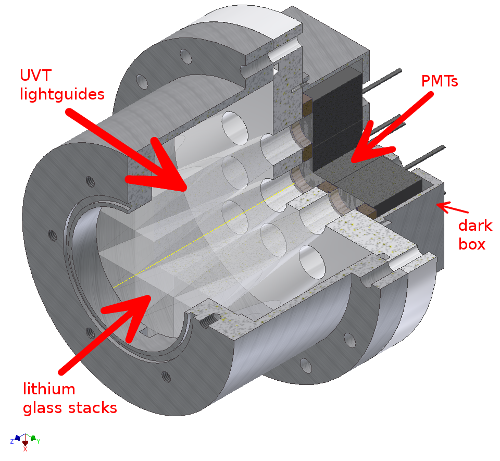
\includegraphics[width=0.49\textwidth]{figures/detdesigned.png} 
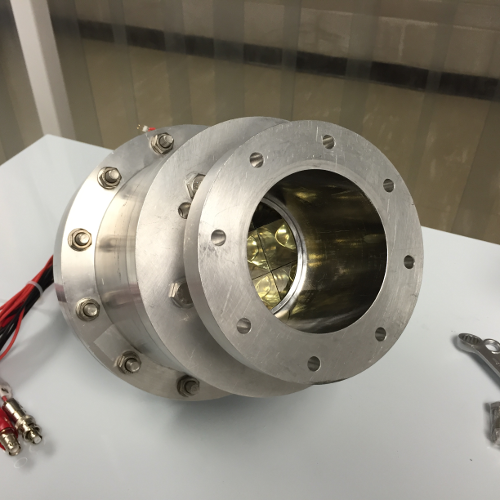
\includegraphics[width=0.49\textwidth]{figures/ucndet.png} 
\caption{\label{fig:detdesigned} Three dimensional drawing of the UCN
  detector and enclosure (top), and a photo of the detector (bottom).}
\end{figure} 

\subsection{$^6$Li Detector Signal Treatment}

Each of the nine pixels of scintillating glass' light is detected by a
Hamamatsu R7600U Photomultiplier Tube (PMT).  The signals from the
PMTs are amplified by a Phillips 775 Octal $10\times$ Preamplifier and
read out by a CAEN v1720 digitizer.

The CAEN v1720 has a PSD firmware to reduce the size of the data read
out, and has eight channels.  The first seven pixels of the detector
are read out on one digitizer, and two pixels, including the centre
pixel, are read out on a second digitizer.  Each of the digitizers was
connected by an independent optical fibre to a CAEN A3818 PCI card on
the DAQ computer for readout, allowing data rates up to 60~MB/s per
link.

The time-stamp provided by the digitizer is a clock cycle count in 4 ns
ticks up to 17 seconds.  To help keep track of the time-stamp
wrap-around, and check the digitizer synchronization, a $1$~Hz pulser
was fed into the last channel of each of the two digitizers.  In
addition a signal from the PSI proton beam timing was sent into one of
the channels of the detector to be used to determine thee times when
the proton beam arrived.

The Data Acquisition (DAQ) software used the MIDAS system that is
commonly used at PSI and TRIUMF.  A MIDAS frontend for the CAEN v1720
was written to collect the PSD data from the digitizers and save it
into midas banks. 

Further details on the digitizer PSD settings can be found in
Section~\ref{sec:digisim}.  


\section{ Scintillation and light-guide background simulation }\label{sec:sim}

In order to build probability distribution functions for late light
events, multiple signal events, and combinations of signal and
background events, a detailed simulation of the voltage pulses from
the lithium glass and of the digitizer PSD was developed.  A single
photo-electron was assumed to produce a Gaussian pulse with an
amplitude drawn from a Gaussian with mean and width, $A=20$~mV, and
accepting only amplitudes above 4~mV.

A single scintillation signal event's pulse was then built assuming
that the arrival times of each photo-electron from the scintillation
signal followed some rise time, $\tau_R=6.4$~ns, a fast scintillation
fall time, $\tau_F=41.7$~ns, and a slow scintillation fall time,
$\tau_S=2000$~ns.  The probability, $P(t)$, of having a photo-electron
at a given time, $t$, when the scintillation light starts arriving at
time, $T$, was drawn from the distribution:
\begin{equation}
  P(t) = \left\{
    \begin{array}{l}
      A ( 1 - {\tt e}^{-(t-T)/\tau_R } ),\ \ T<t<T+5\tau_R \\
      A ( (1-f_L) {\tt e}^{ -(t-T-5\tau_R)/\tau_F } +   \\
      \ \ f_L {\tt e}^{ -(t-T-5\tau_R)/\tau_L } ),\ \  t>=T+5\tau_R.
    \end{array}
    \right.
\end{equation}
The fraction of the scintillation light in the late light was
$f_L=1$\%.  All of the values used in the simulation, as described
above, were chosen to best match the data.  The number of
photo-electrons for a single neutron event was drawn from a Poisson
distribution with mean number of photo-electrons of 83.  The
distribution of scintillation photo-electron arrival times along with
a sample pulse is shown in the left panel of Fig.~\ref{fig:signalpdf}.

\begin{figure}[!htpb]
\centering
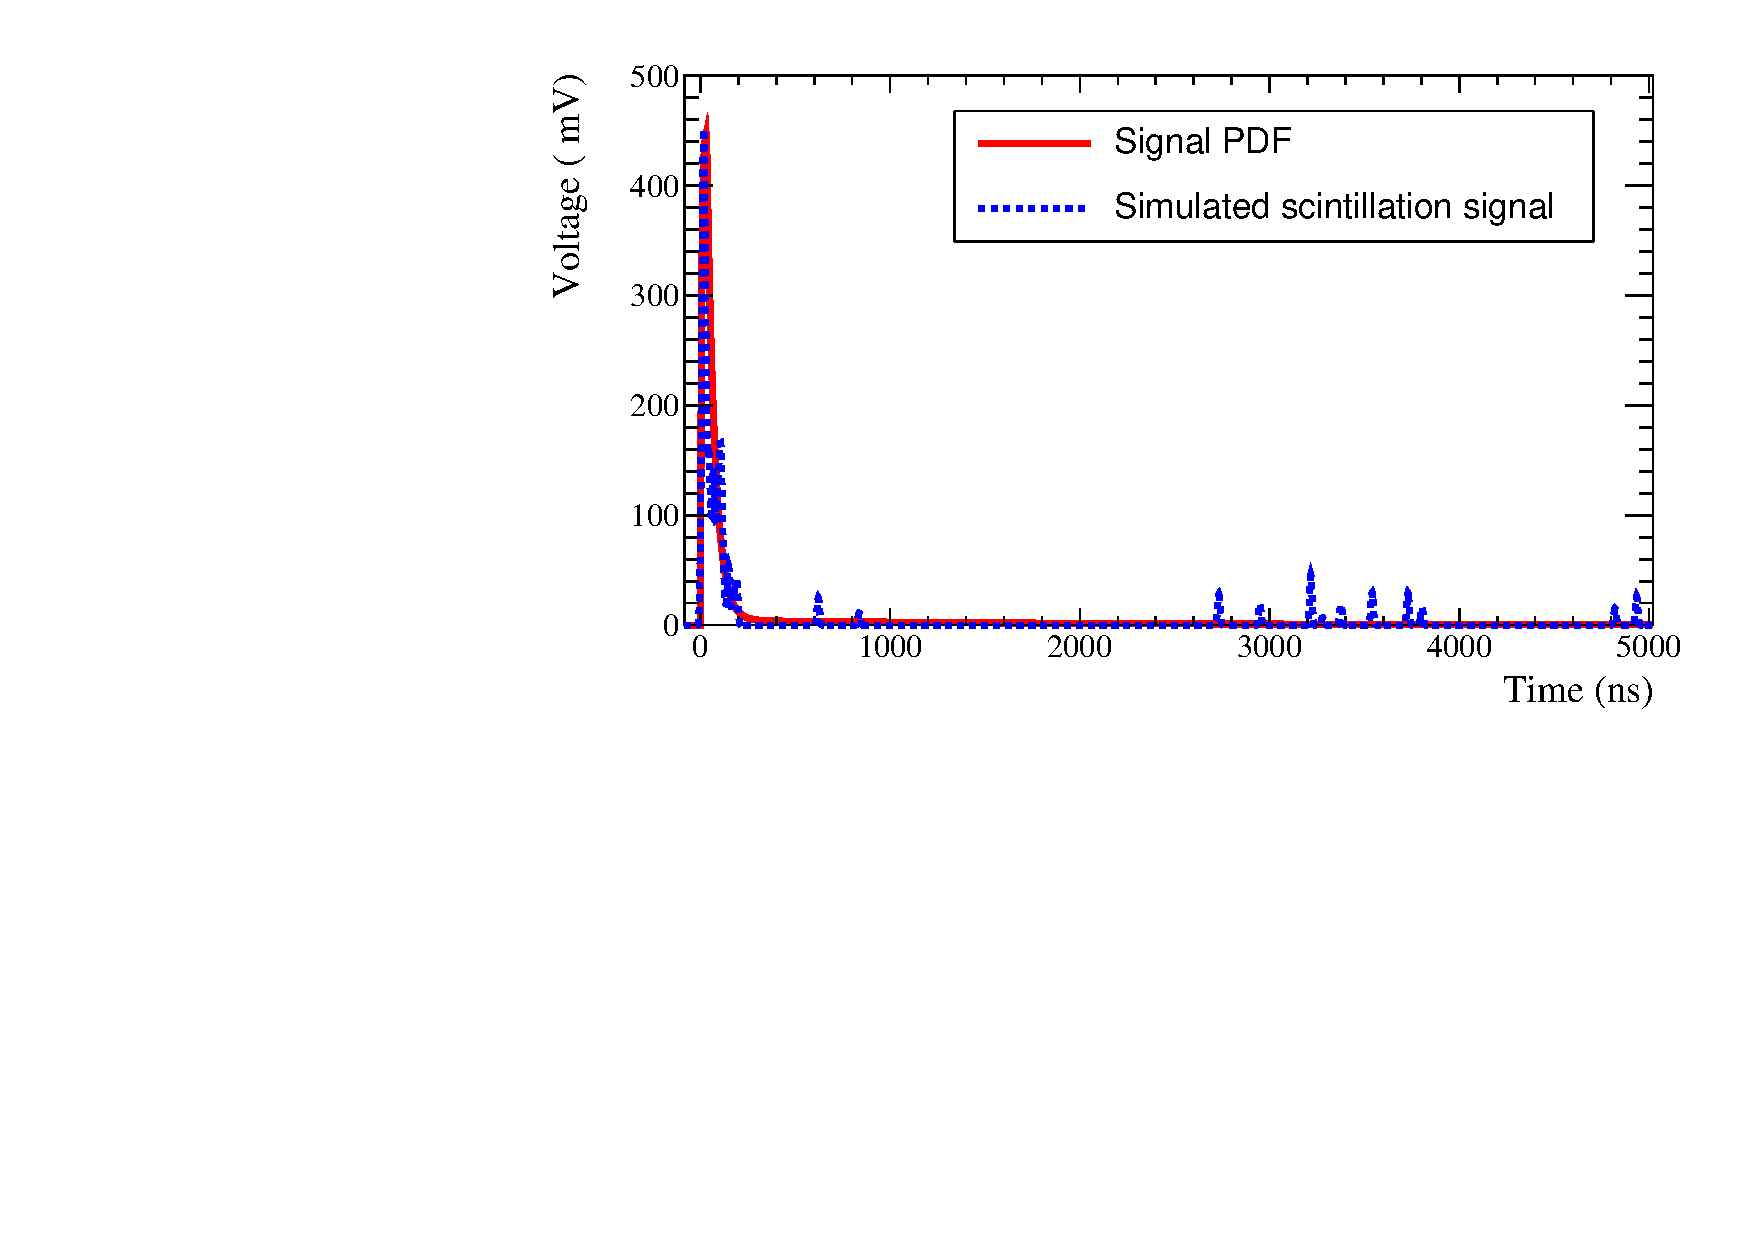
\includegraphics[width=0.49\textwidth]{figures/signalpulse.pdf}
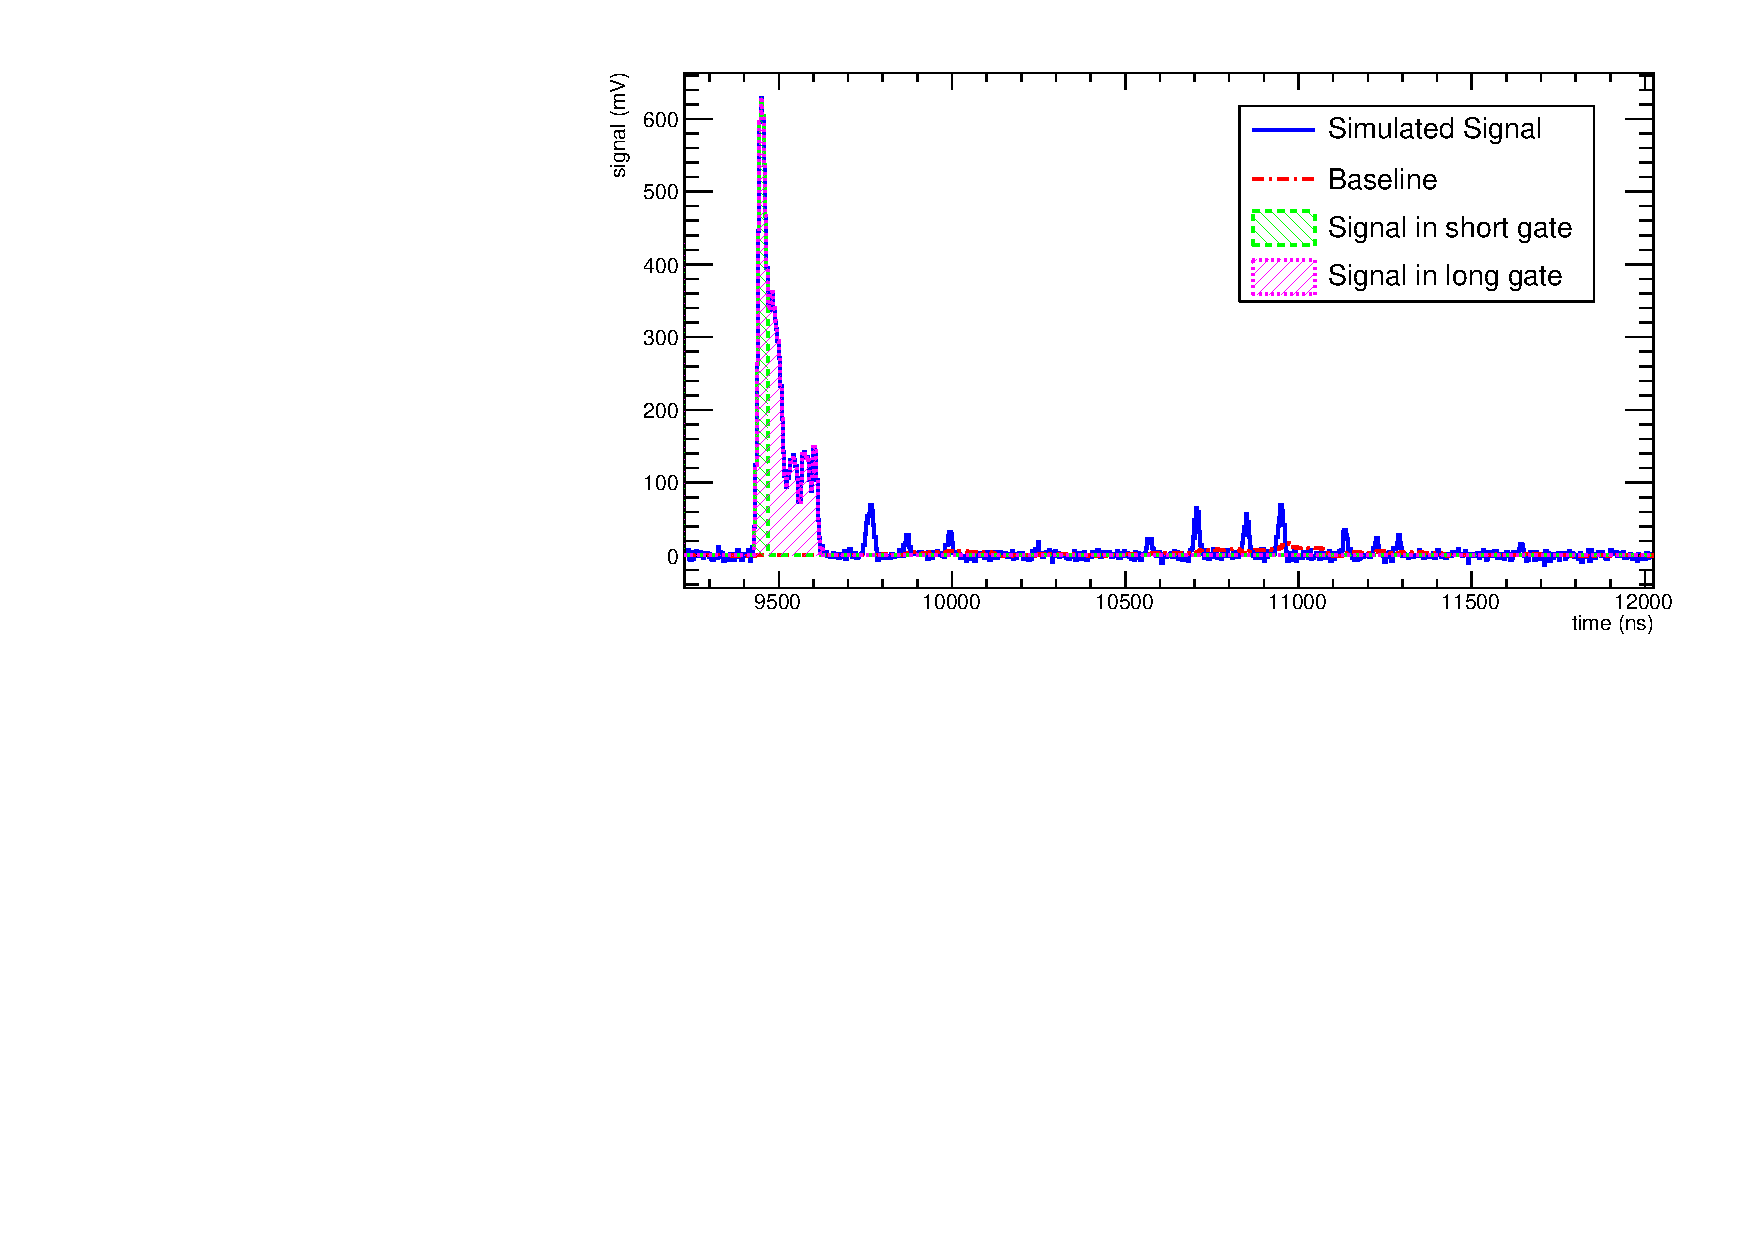
\includegraphics[width=0.49\textwidth]{figures/digisimexample.pdf}
\caption{ Simulated scintillation signal (blue dashed) and
  distribution function used to generate it (red solid) is shown in
  the left panel.  The right panel shows the digitizer treatment of
  another simulated signal (solid line), where the baseline
  calculation (red dot-dashed line), signal within the short gate
  (green right-diagonal fill) and signal within the long gate (magenta
  left-diagonal fill) are shown.}\label{fig:signalpdf}
\end{figure}

A single background event was modelled as having a Gaussian pulse with
$\sigma=6.4$~ns for the times of each photo-electron.  Again, each
photo-electron was treated as a Gaussian with a random amplitude drawn
from a Gaussian with mean and width of $A=20$~mV, and accepting only
amplitudes above 4~mV.  The number of photo-electrons for the
background signal was drawn from an exponential distribution with an
average of $7.5$ photo-electrons.  This distribution was chosen to match
the dominant component of the background observed in data.

The simulation of the pulses was used to generate 0.1 second long sets
of data where the signal and background pulses were generated at a
specified random rate.  These simulated data were then sent to a
digitizer simulation, described in the following section.


\subsection{ Digitizer simulation }\label{sec:digisim}
 
The CAEN V1720 digitizer with the PSD firmware samples the waveforms
every 4~ns, and for each sample digitizes the voltage on a $\pm 1$~V
scale into an ADC value between 0 and 4096.  Each channel of the
digitizer can trigger on its signal based on going some number of ADC
counts below a pedestal value.  In the simulation the threshold was
set at 250 ADC ($\sim 125$~mV).  The digitizer can be be run with a
fixed pedestal, or simpler to set up, a pedestal taken from an average
over the last 32 samples.  This self calculated pedestal is called a
baseline in the digitizer documentation, and once a trigger happens,
the baseline is held constant until the end of a specified gate time.

The PSD firmware calculates the sum of the signal below the threshold
for a short gate width, $t_s=40$~ns, and for a long gate width,
$t_L=200$~ns, after the trigger.  The ADC sum below threshold within
the short gate is called, $Q_S$, and the sum within the long gate is
called, $Q_S$.  The PSD value is also calculated, and defined as:
\begin{equation}
{\tt PSD} = \frac{ (Q_L - Q_S)} { Q_L }.
\end{equation}
After each trigger, the digitizer channel is busy for a 150~ns
dead-time.  An example of the signal within each of the gates is
depicted in the right panel of Fig.~\ref{fig:signalpdf}.  A cut on the
values of the charges $Q_L$ and PSD provides a rejection of gamma
interactions with the lighguides.

As outlined in the section describing the rates seven categories of
events are considered.  Simulated electronic pulses for each of these
possible combinations is shown in Fig.~\ref{fig:eventTypes} and
Fig.~\ref{fig:eventTypes2}.

\begin{figure}[!htpb]
\centering
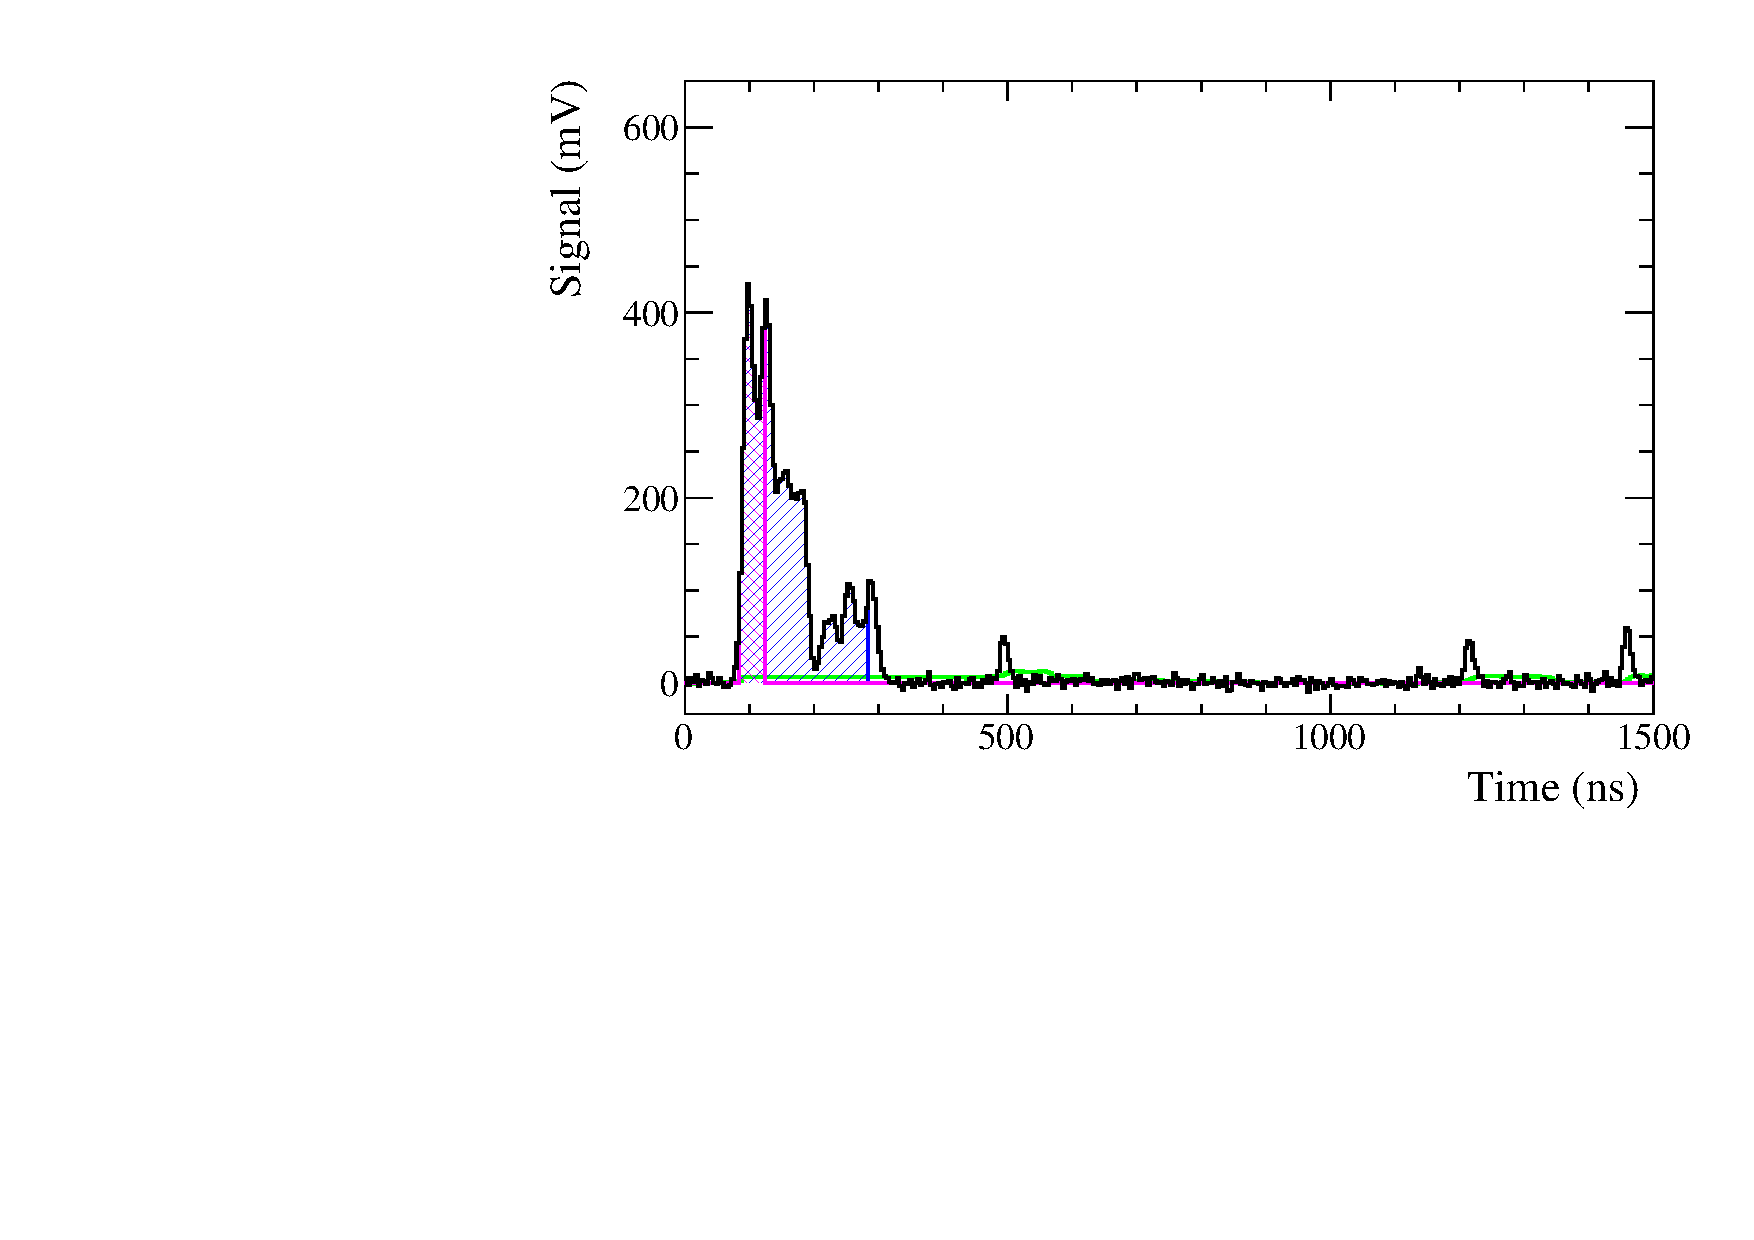
\includegraphics[width=0.45\textwidth]{figures/signal1.pdf}
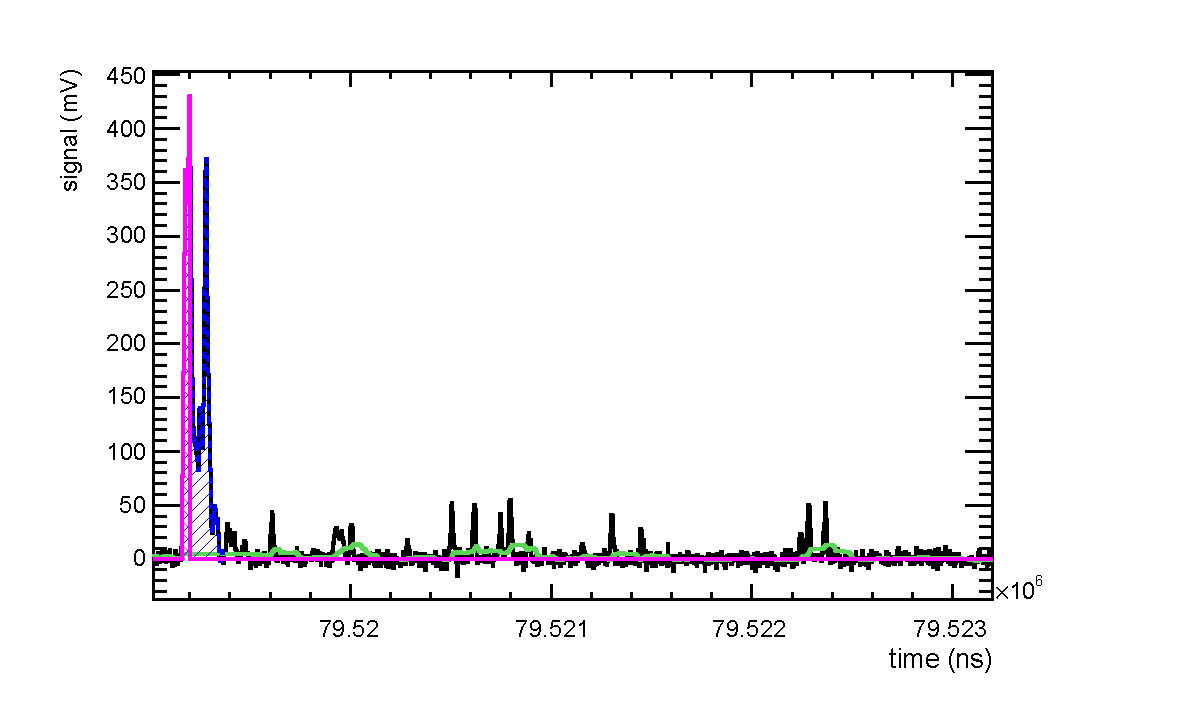
\includegraphics[width=0.45\textwidth]{figures/mixed1.pdf}
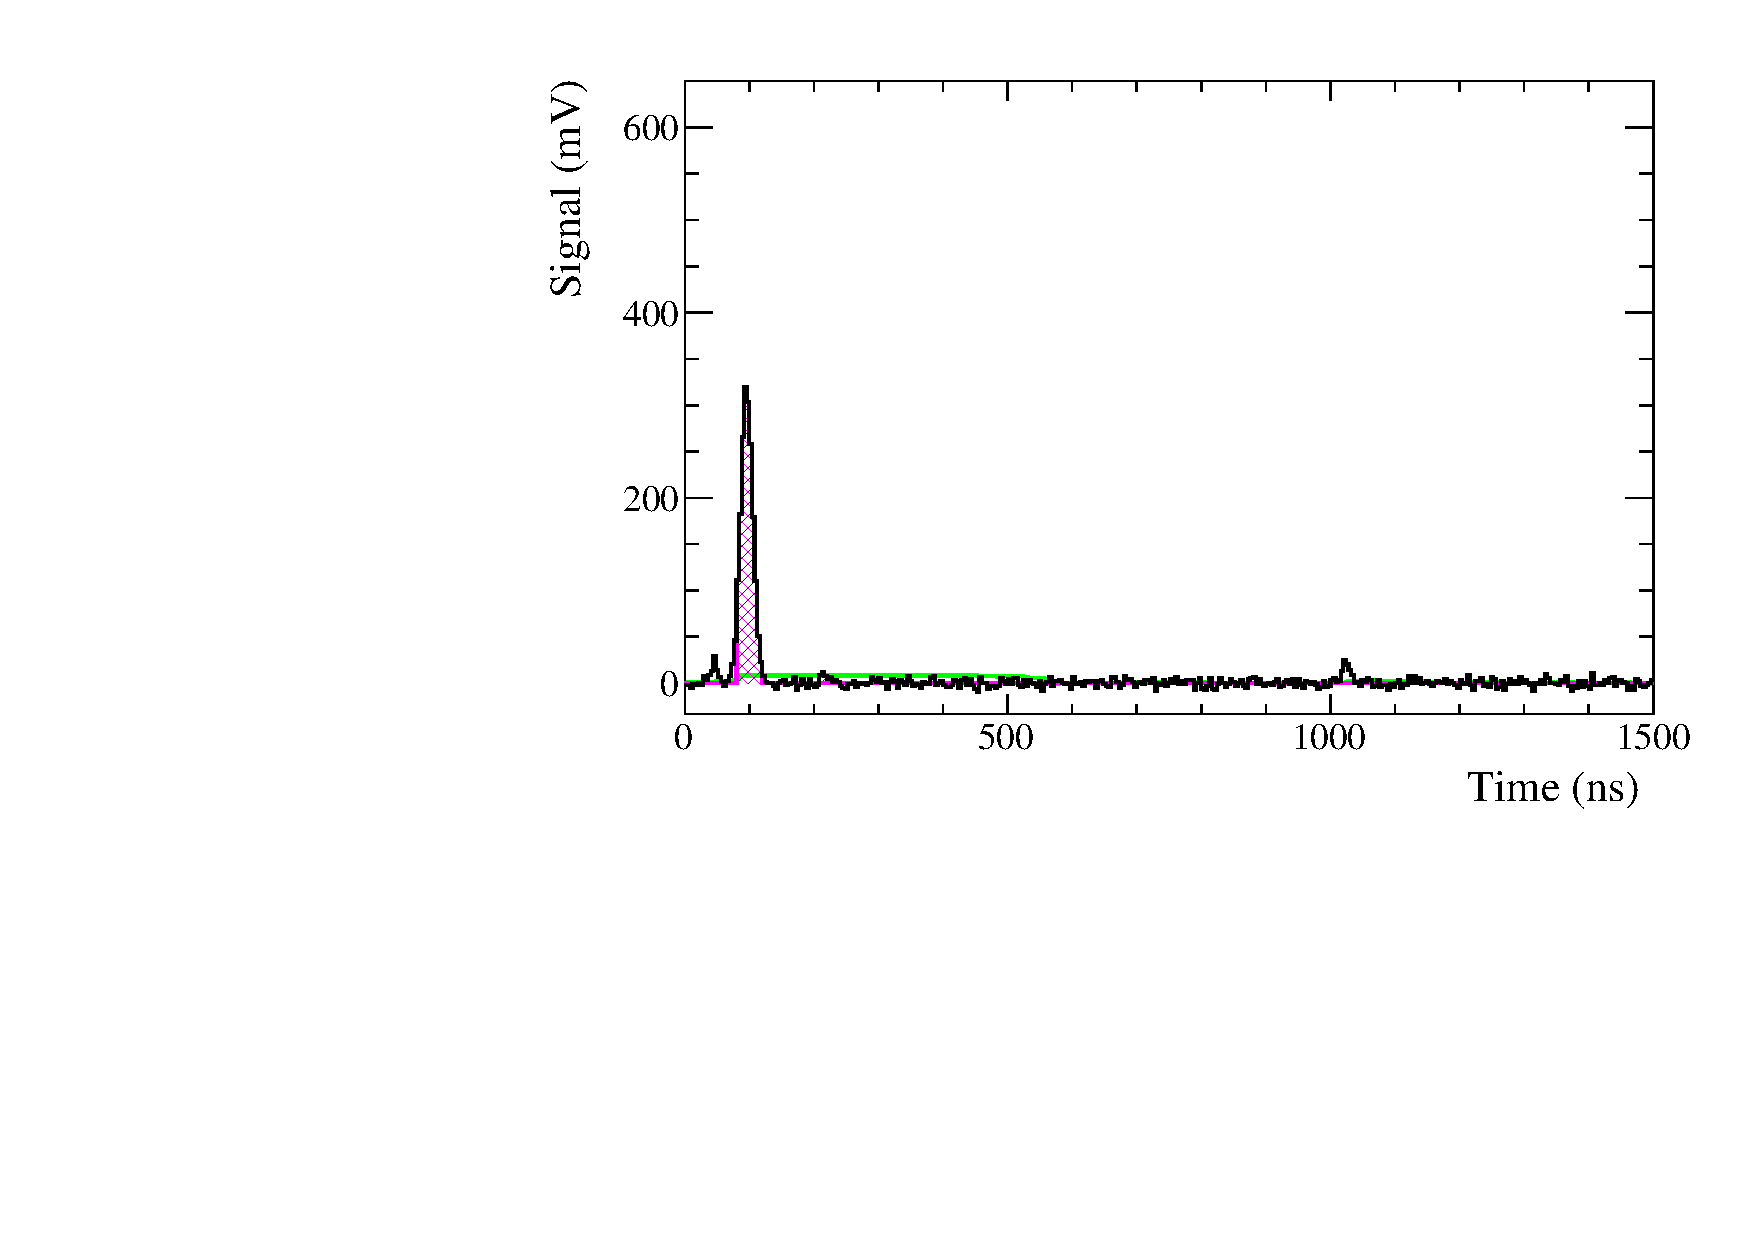
\includegraphics[width=0.45\textwidth]{figures/gamma1.pdf}
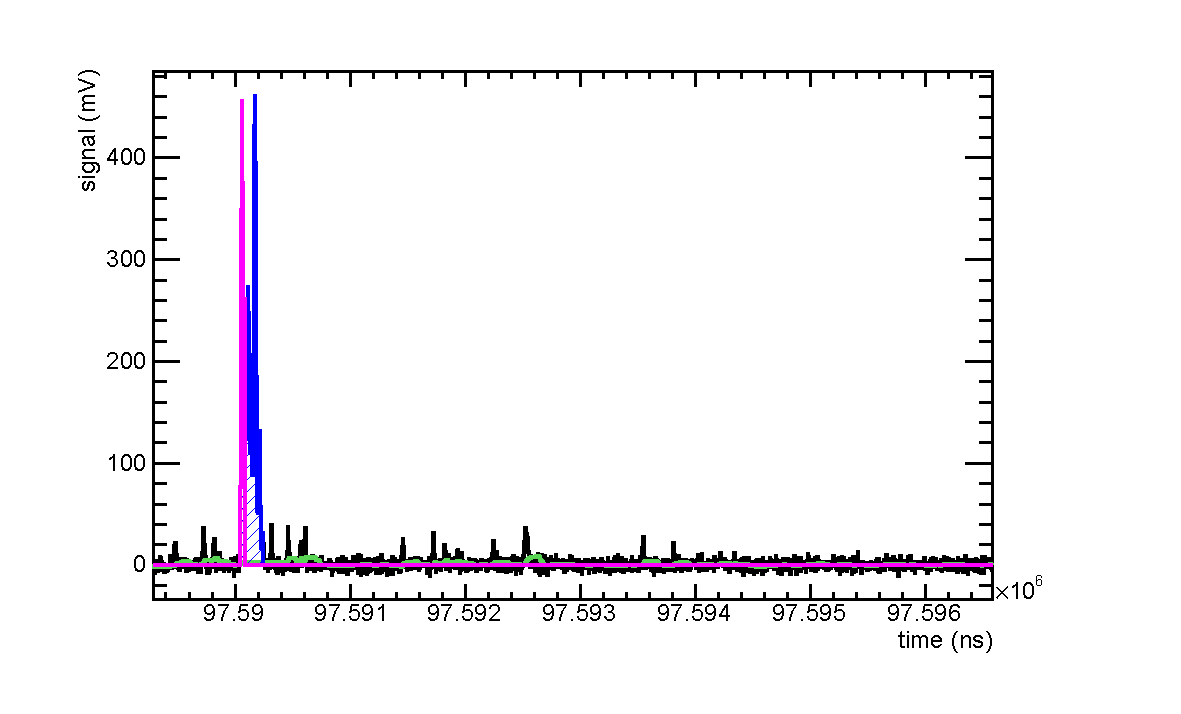
\includegraphics[width=0.45\textwidth]{figures/gammapileup1.pdf}
\caption{ Simulated signals seen by the $^{6}$Li detector in mV versus
  time for different combinations of signal and background events.
  The magenta left-diagonal-hatched region represents the $Q_S$
  portion of the signal, the blue right-diagonal-hatched region
  represents $Q_L$, and the green line (colour online) represents the
  average baseline.  From top to bottom right the plots show: a single
  signal event, a multiple signal event, a single background event,
  and a multiple background event. }\label{fig:eventTypes}
\end{figure}


\begin{figure}[!htpb]
\centering
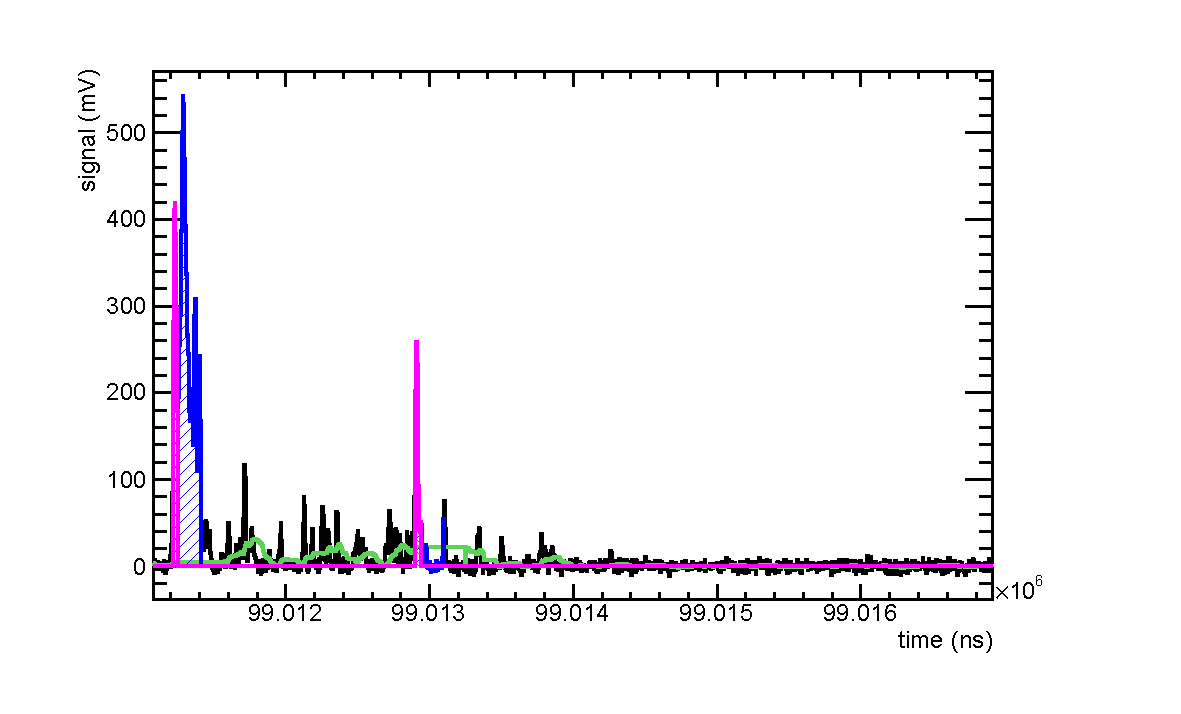
\includegraphics[width=0.49\textwidth]{figures/pileup1.pdf}
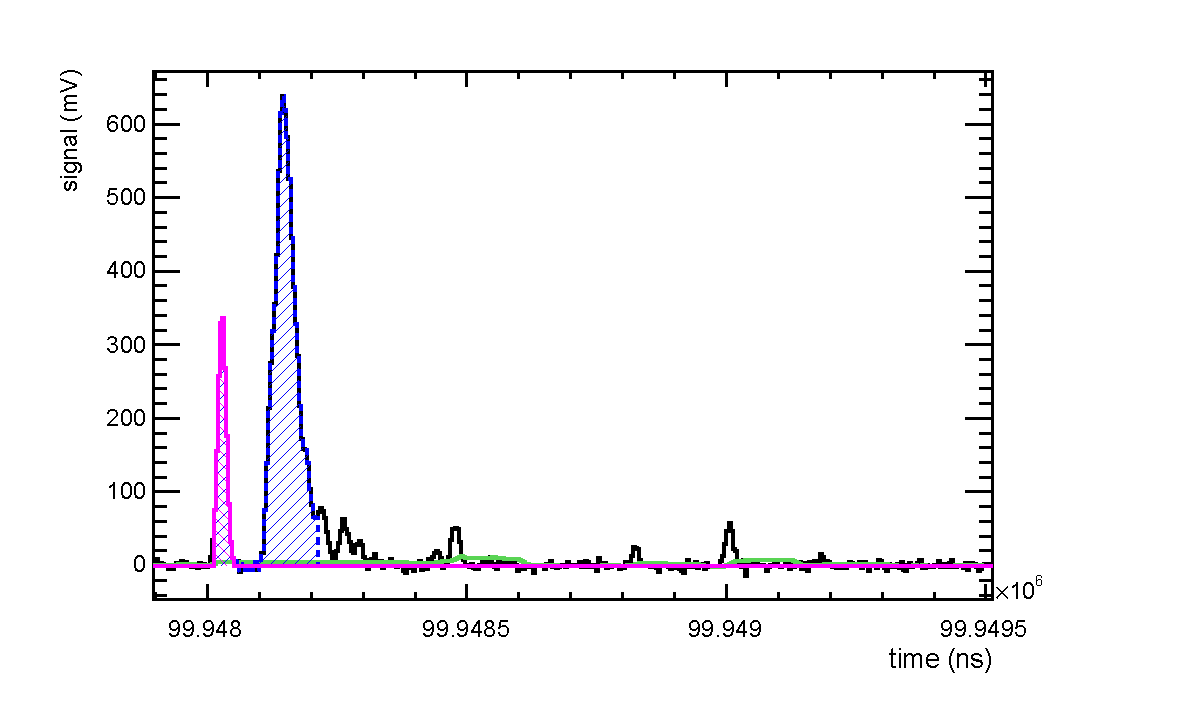
\includegraphics[width=0.49\textwidth]{figures/retrig1.pdf}
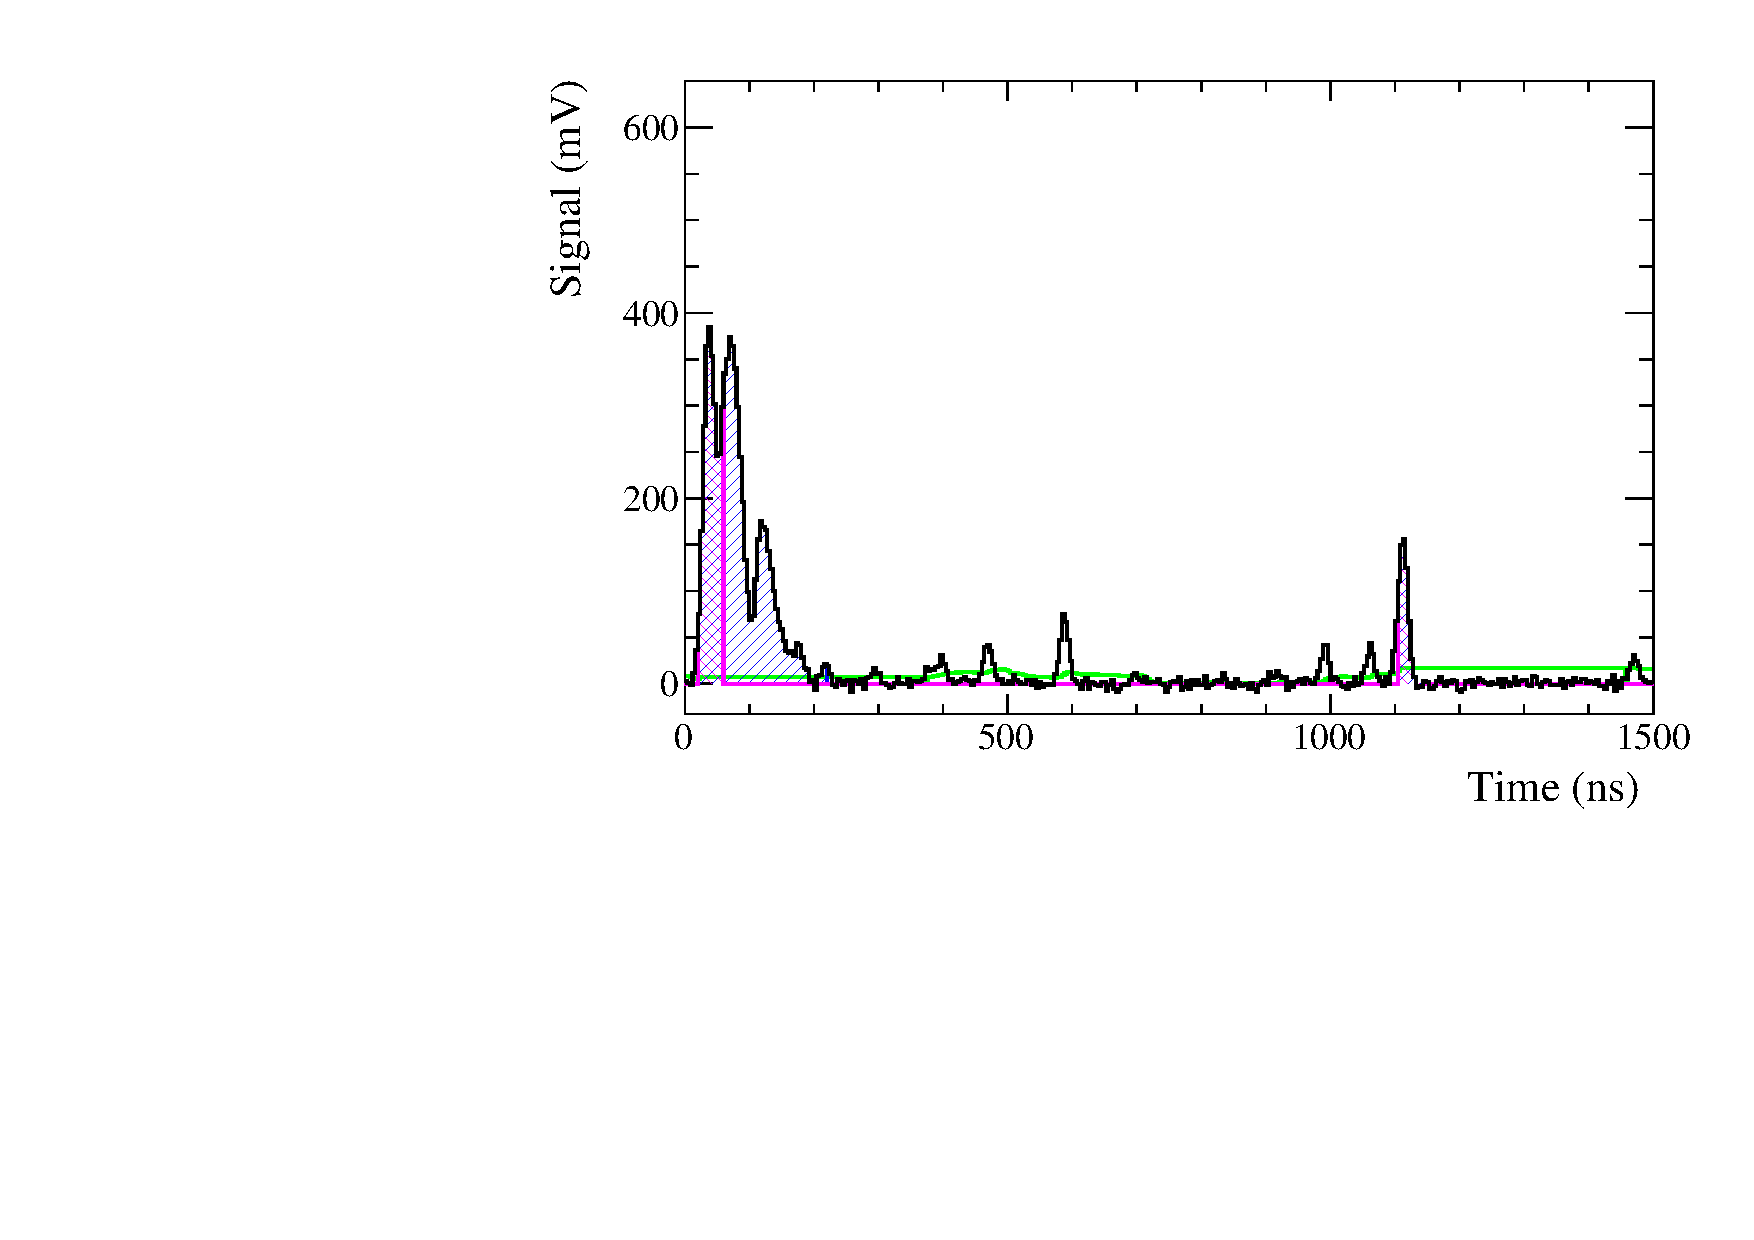
\includegraphics[width=0.3\textwidth,angle=-90]{figures/latelight1.pdf}
\caption{ From top to bottom these plots show: a single signal plus
  single background event, a dead-time event, and a late-light
  re-trigger event. }\label{fig:eventTypes2}
\end{figure}



\subsection{ Probability distribution functions from the simulations }

The combination of the signal and background pulse simulations with
the digitizer simulation is used to generate probability distribution
functions in the PSD versus $Q_L$ space for each of the different
possible combinations of events.

To limit the number of possible PDFs, an approximation of the higher
event multiplicities within a single gate is included in a single PDF.
These multiple signal or multiple background PDFs could change shape
if the rate of events is changed by over a few orders of magnitude,
but is treated as fixed in estimating the detector performance.

Using a collection of randomly generated signal and background events,
the PDFs for each of the signal types was generated.  In the case of
the single background event, it was possible to use the data from beam
cycles with proton-beam off, when there was no UCN produced.  The rest
of the PDFs were generated after tuning the simulation to match the
data.  In the simulation the average number of photo-electrons per
neutron capture, the fall time of the fast scintillation signal, the
fall time of the long scintillation signal, the average number of
photo-electrons in the background were all tuned.  In addition, the
average charge in the signal measured by the detector, from each
channel, was scaled to match the mean value in the simulation (as a
gain matching).

The PDFs for the different combinations of signal and background are
compared to data as shown in Fig.~\ref{fig:eventSpectra}.  A template
fit of these PDFs to estimate amount of signal and background in the
data is possible.


\begin{figure}[!htpb]
\centering
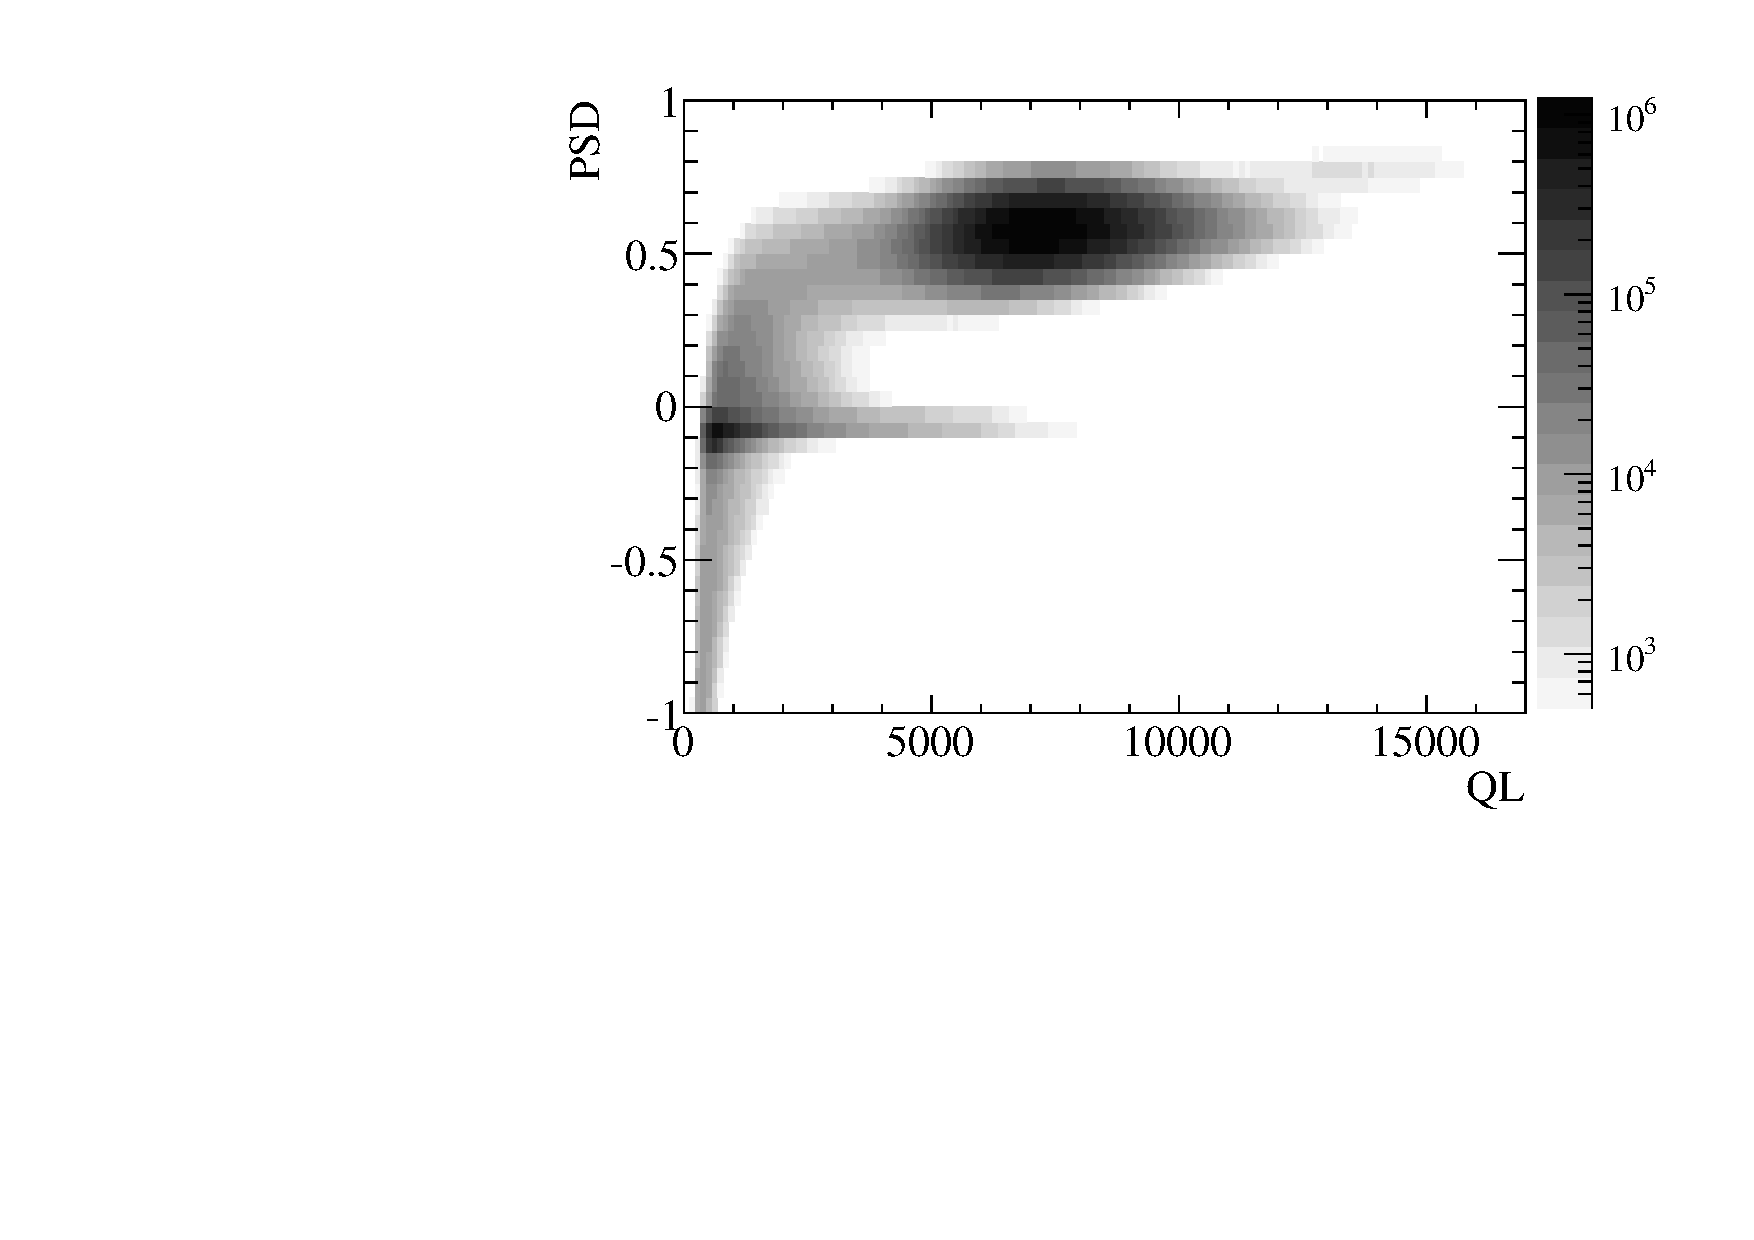
\includegraphics[width=0.45\textwidth]{figures/2DGrayscale.pdf}
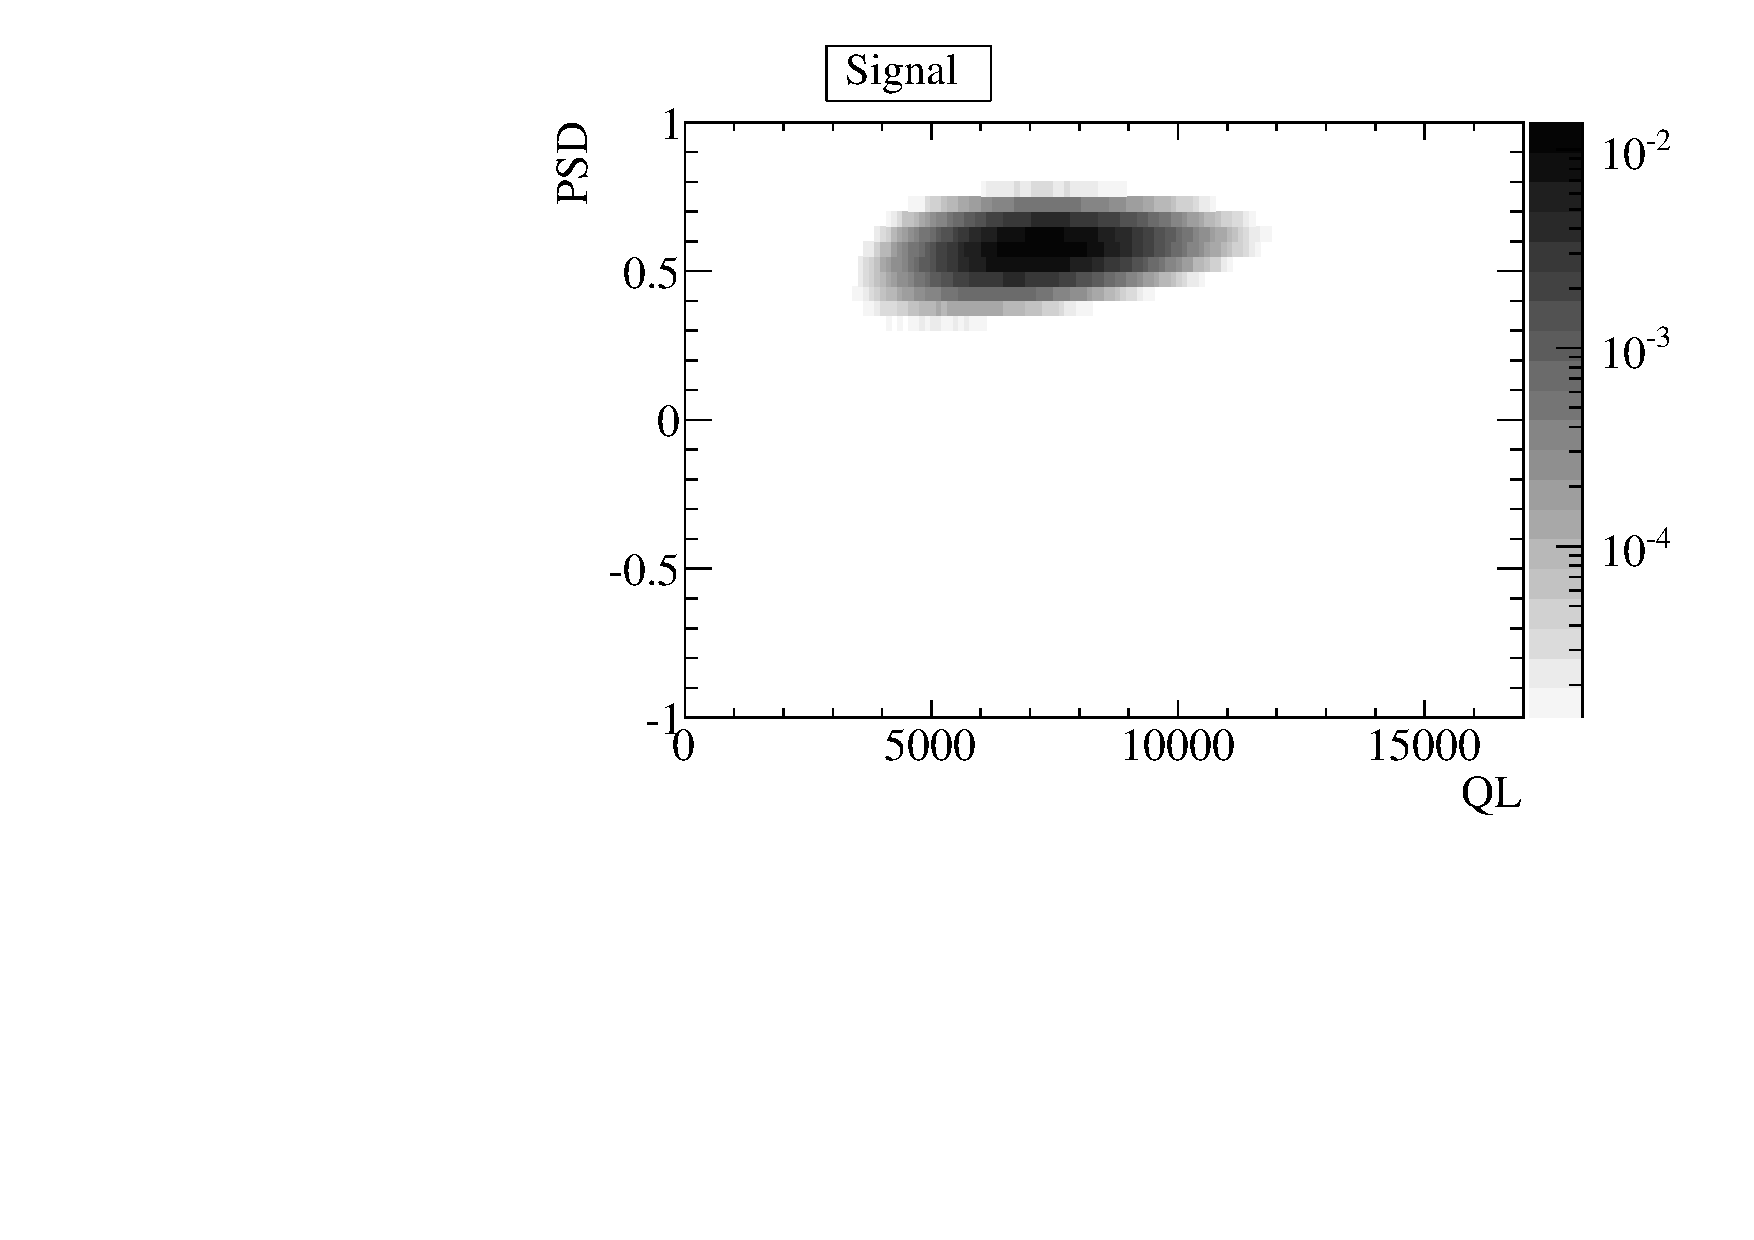
\includegraphics[width=0.45\textwidth]{figures/hsig_psdql.pdf}
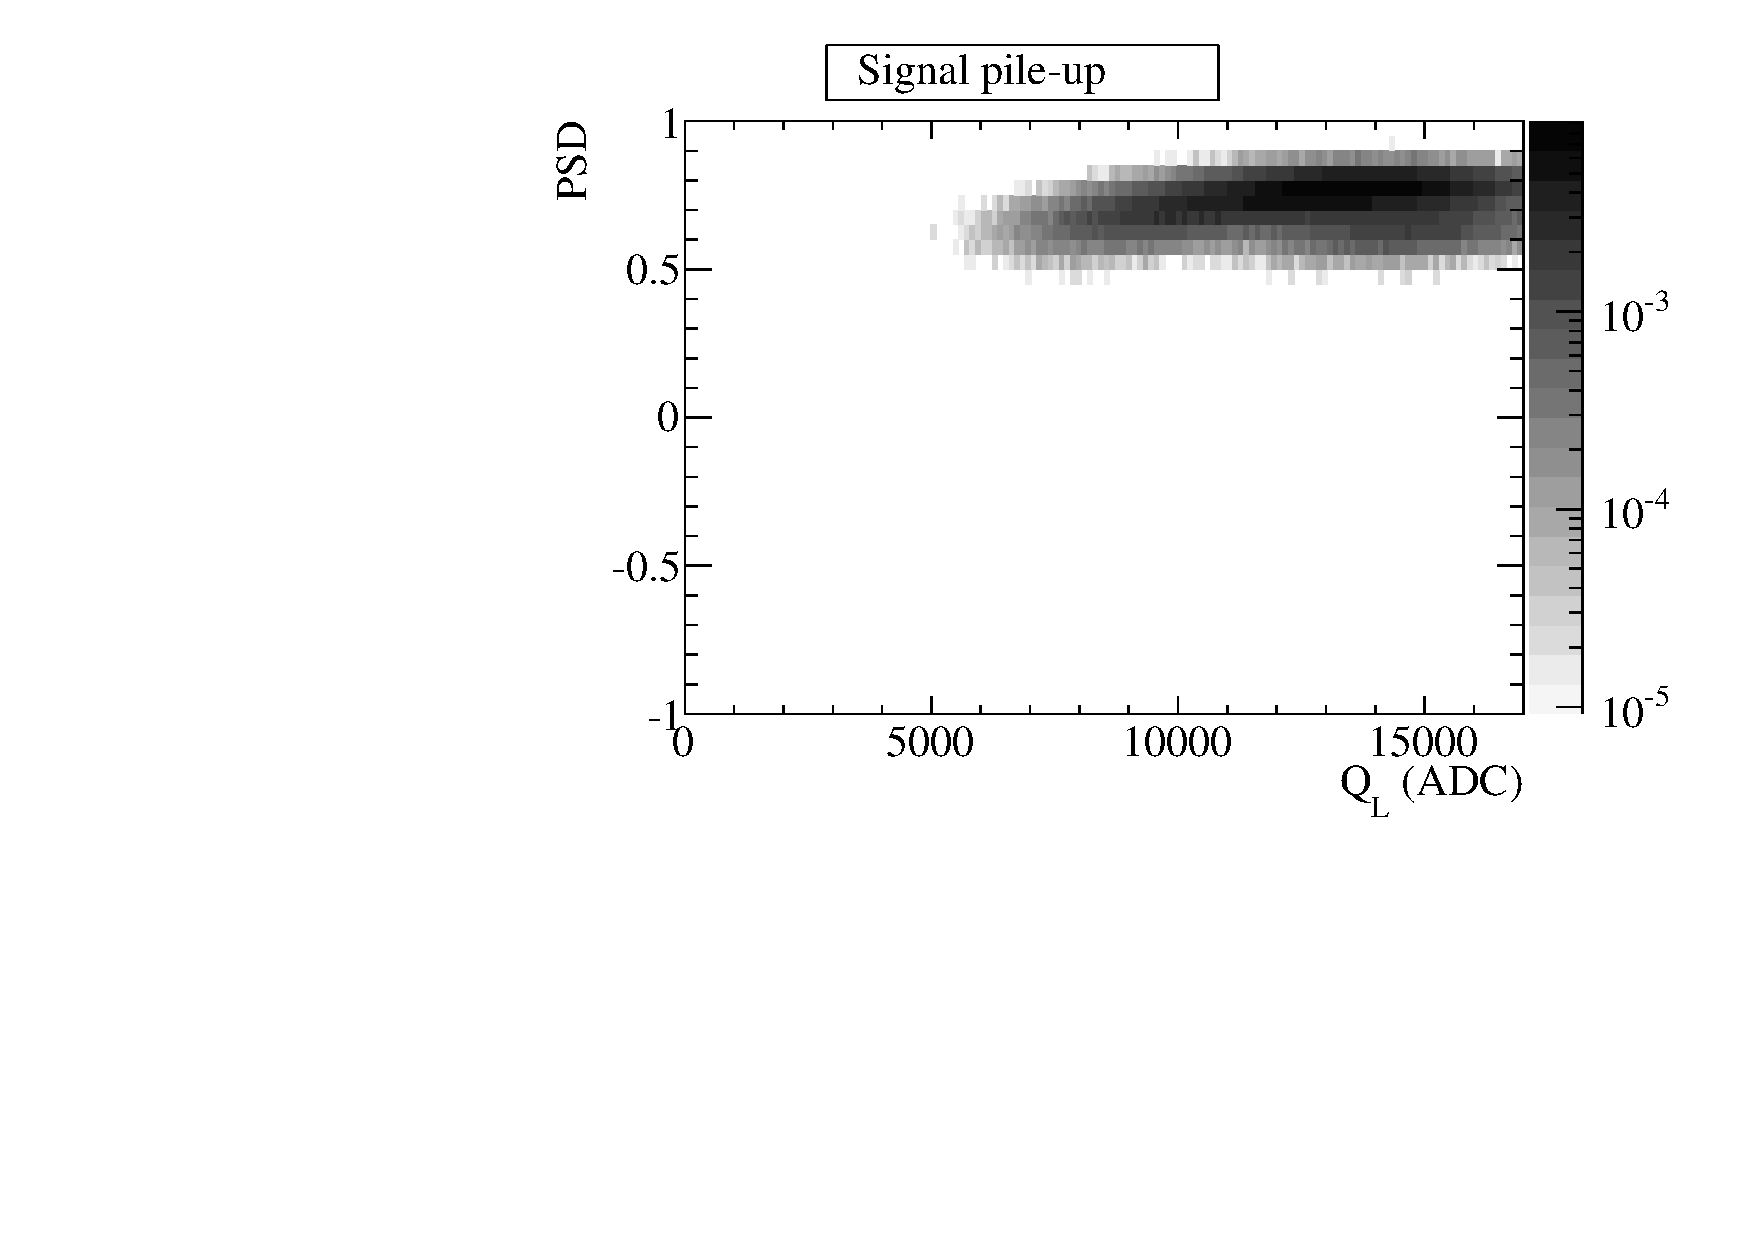
\includegraphics[width=0.45\textwidth]{figures/hsigpile_psdql.pdf}
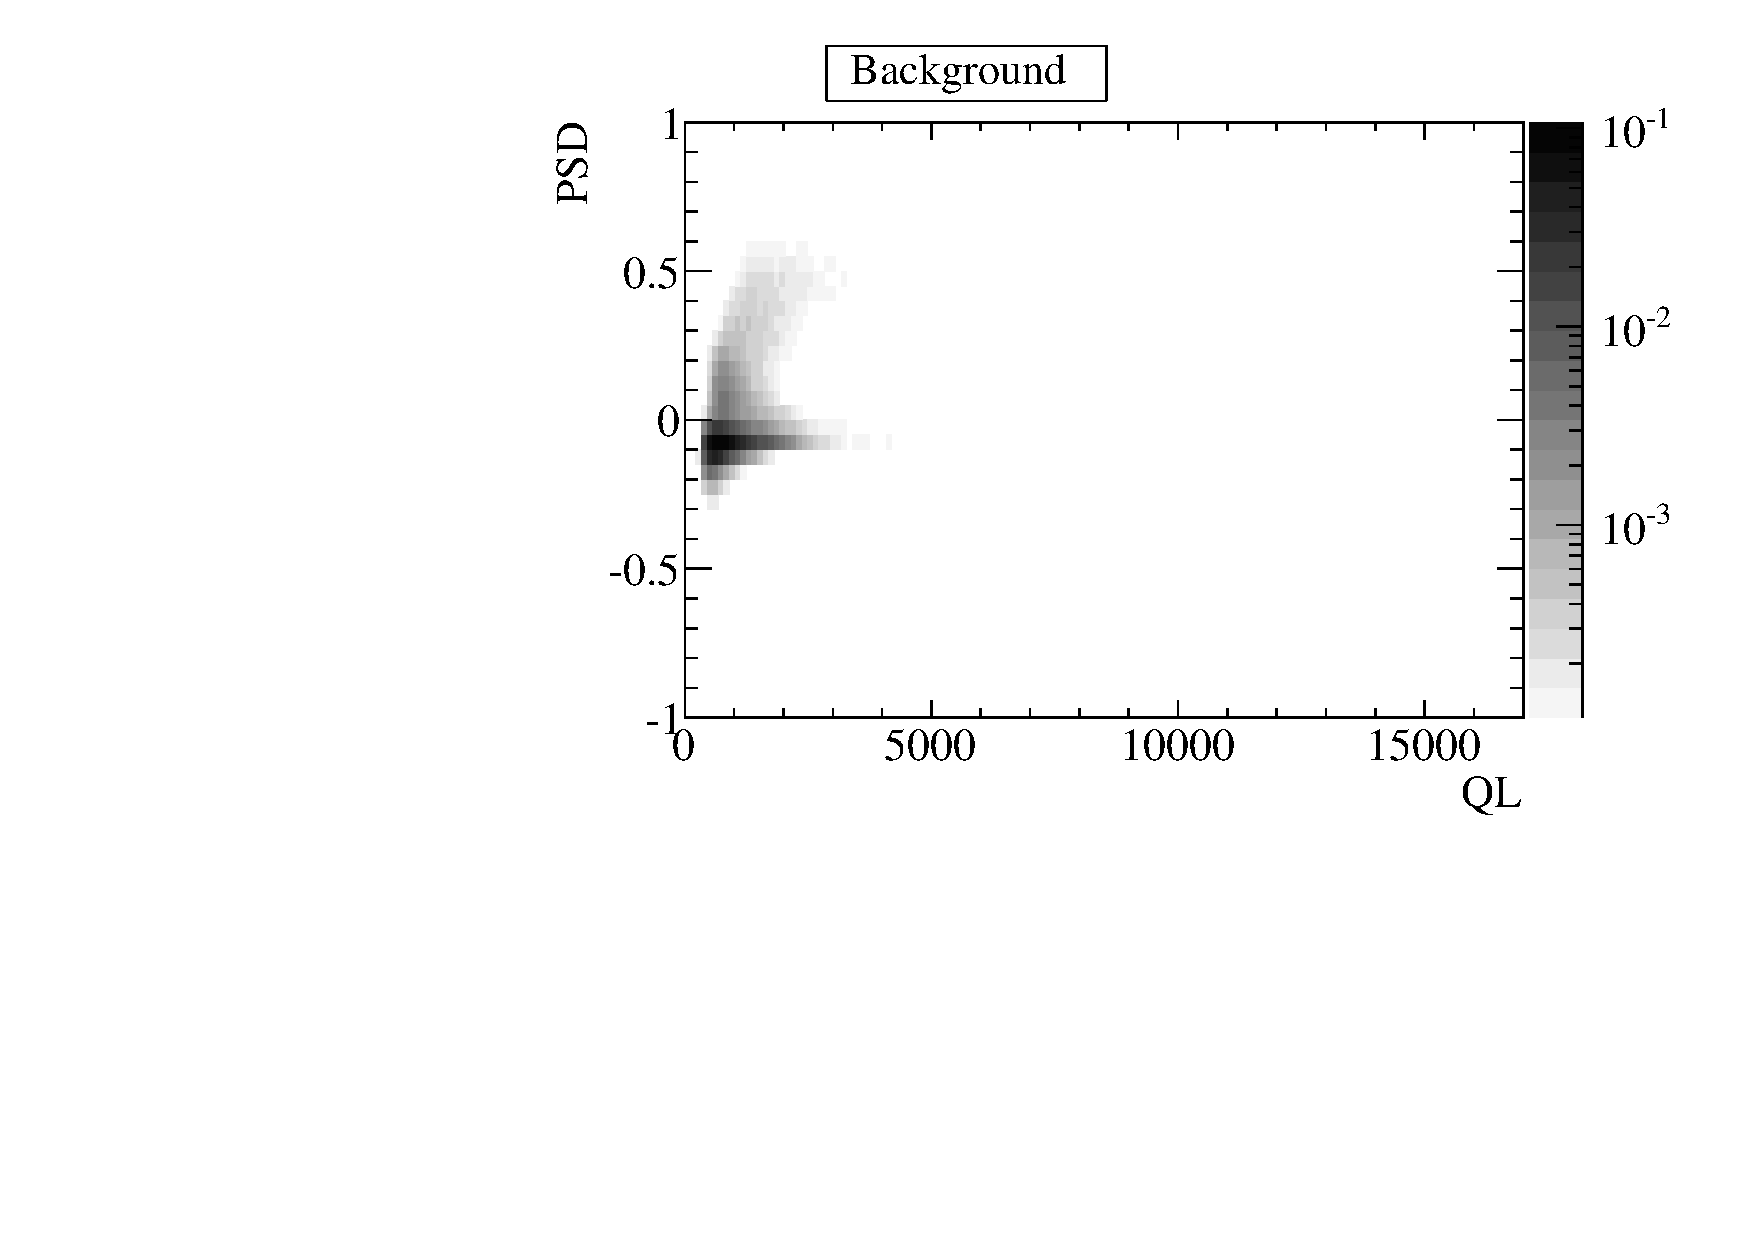
\includegraphics[width=0.45\textwidth]{figures/hbg_psdql.pdf}
\caption{ Event count (or relative event count) as a function of PSD
  and $Q_L$, going from top to bottom is for UCN data,
  single neutron simulation, N neutron simulation, and background (from
  data taken during cycles without proton beam).} \label{fig:eventSpectra}
\end{figure}


\begin{figure}[!htpb]
\centering
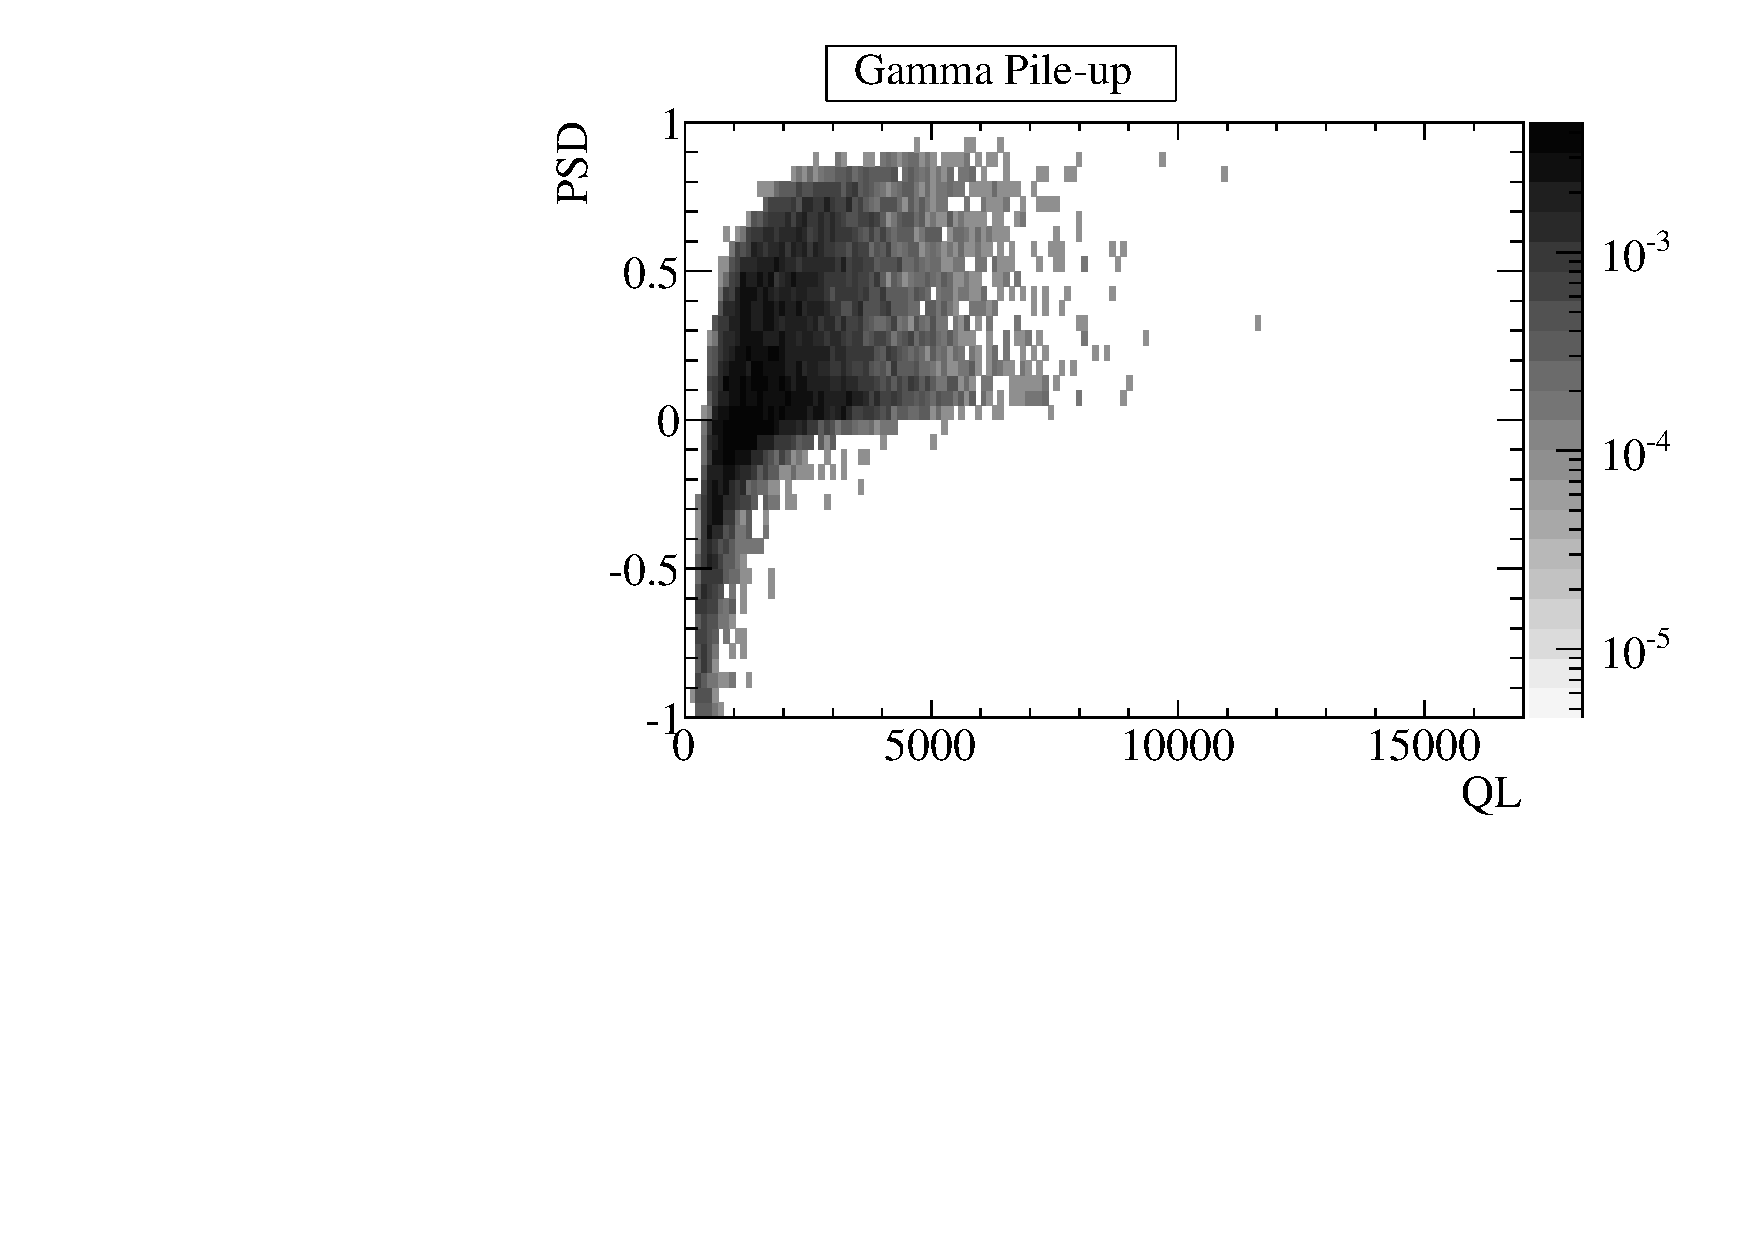
\includegraphics[width=0.45\textwidth]{figures/hbgpile_psdql.pdf}
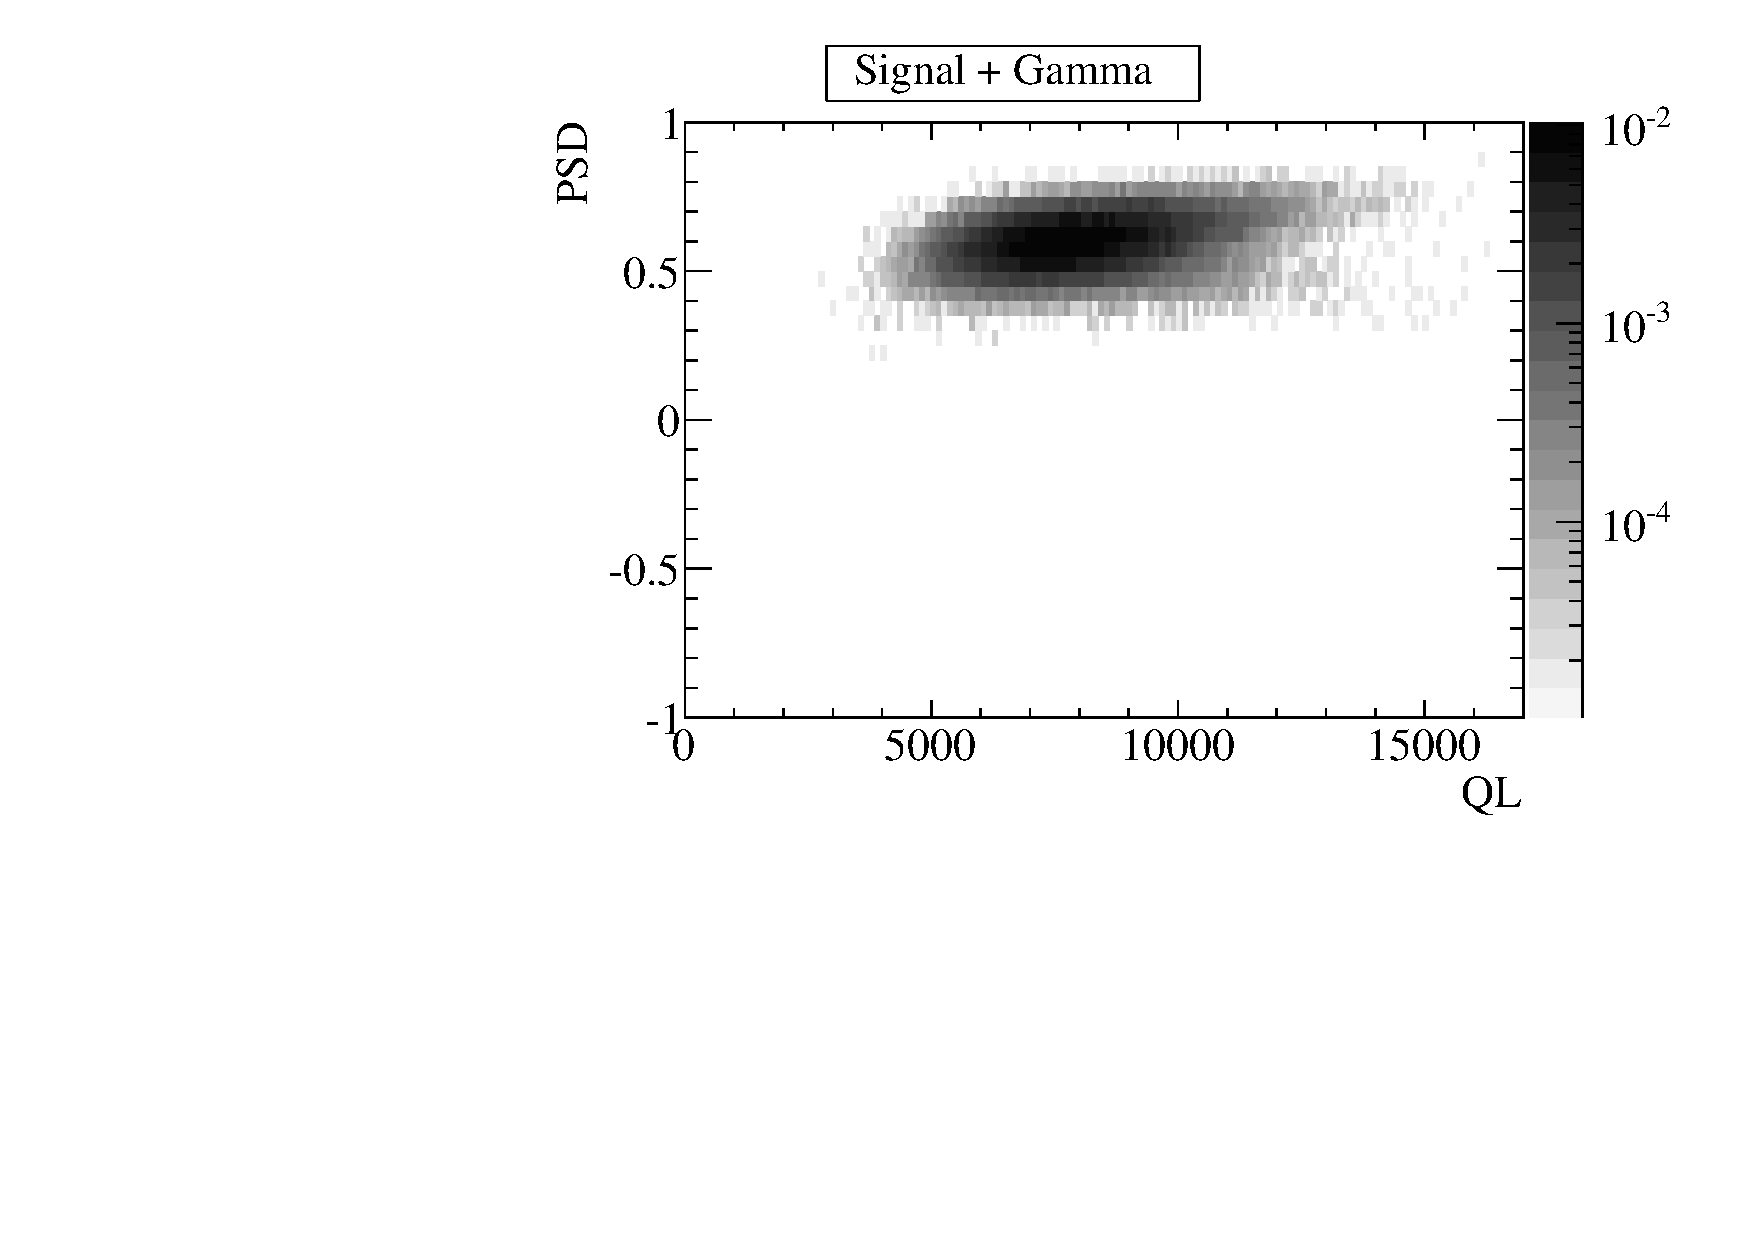
\includegraphics[width=0.45\textwidth]{figures/hsigbg_psdql.pdf}
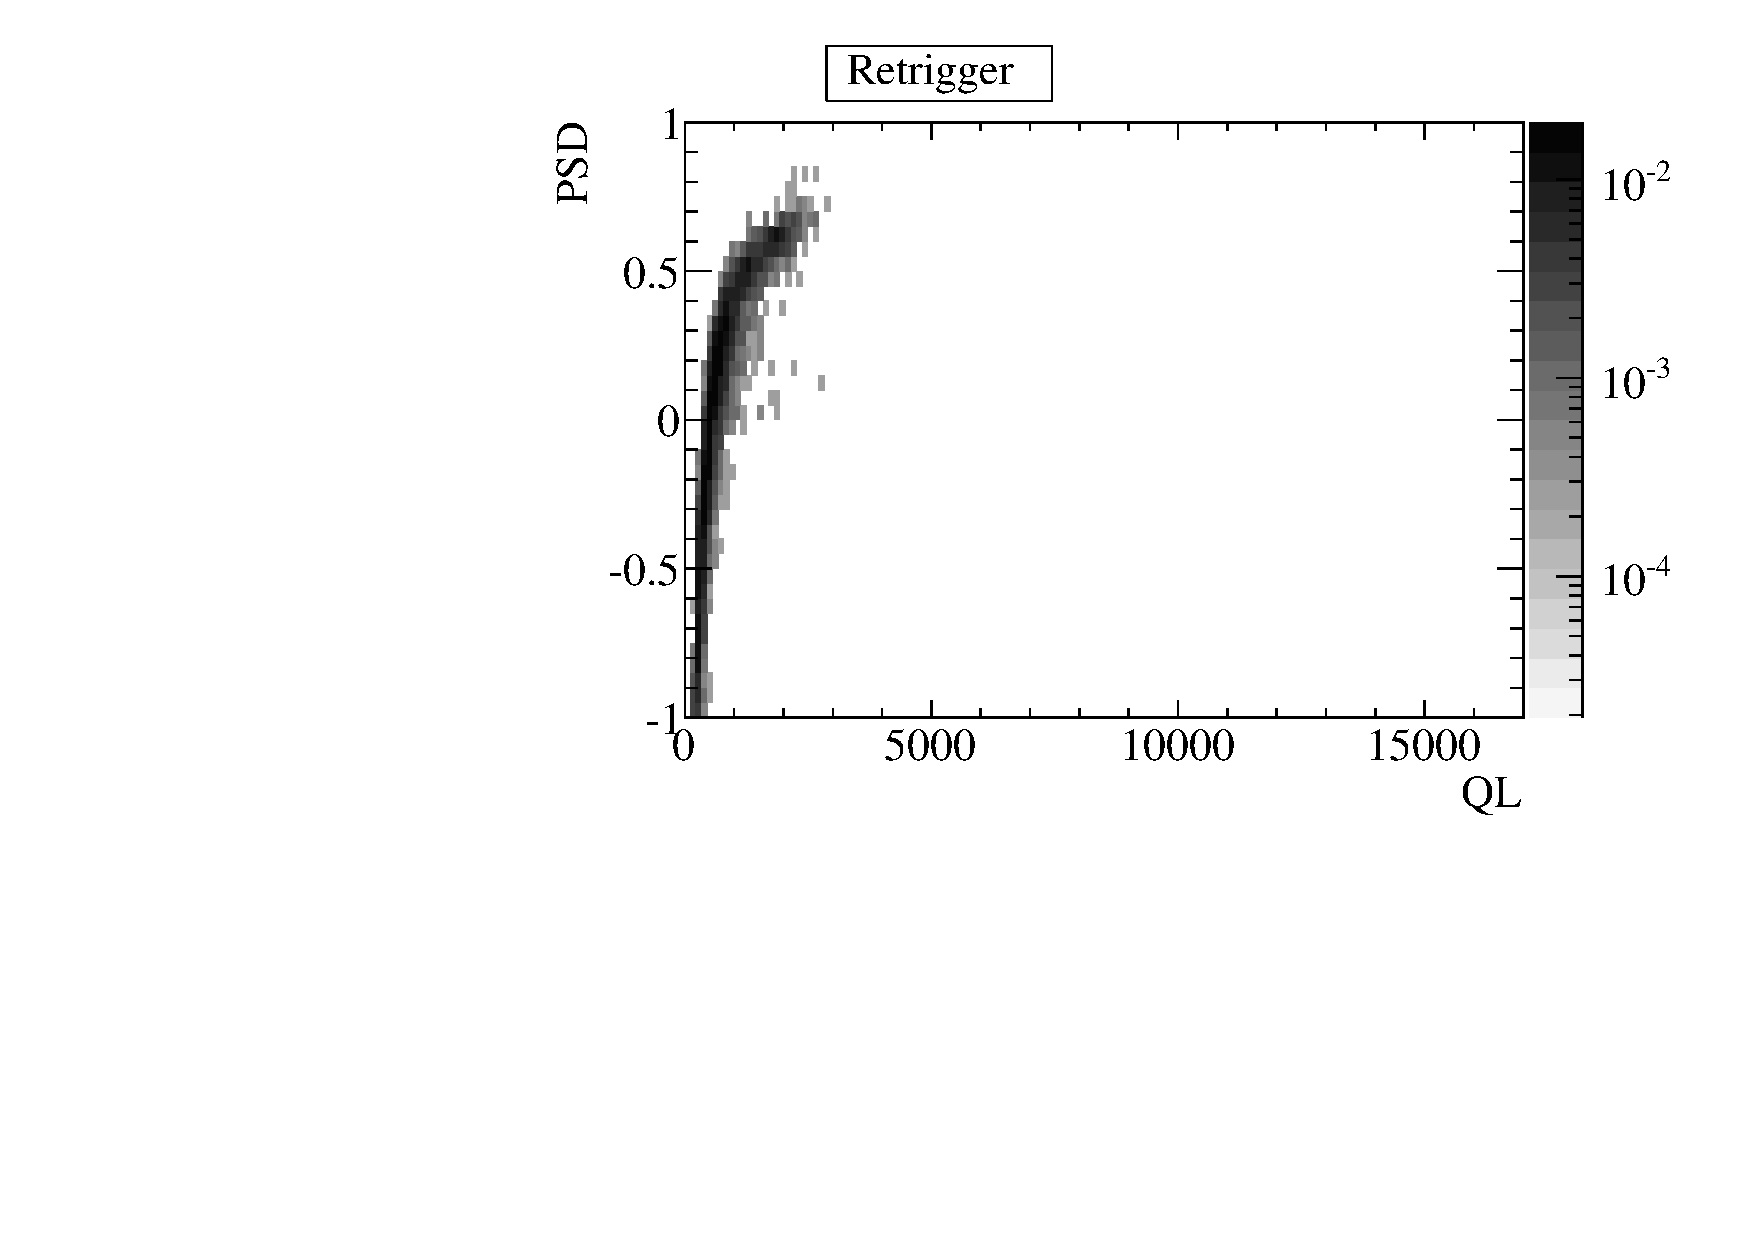
\includegraphics[width=0.45\textwidth]{figures/hretrig_psdql.pdf}
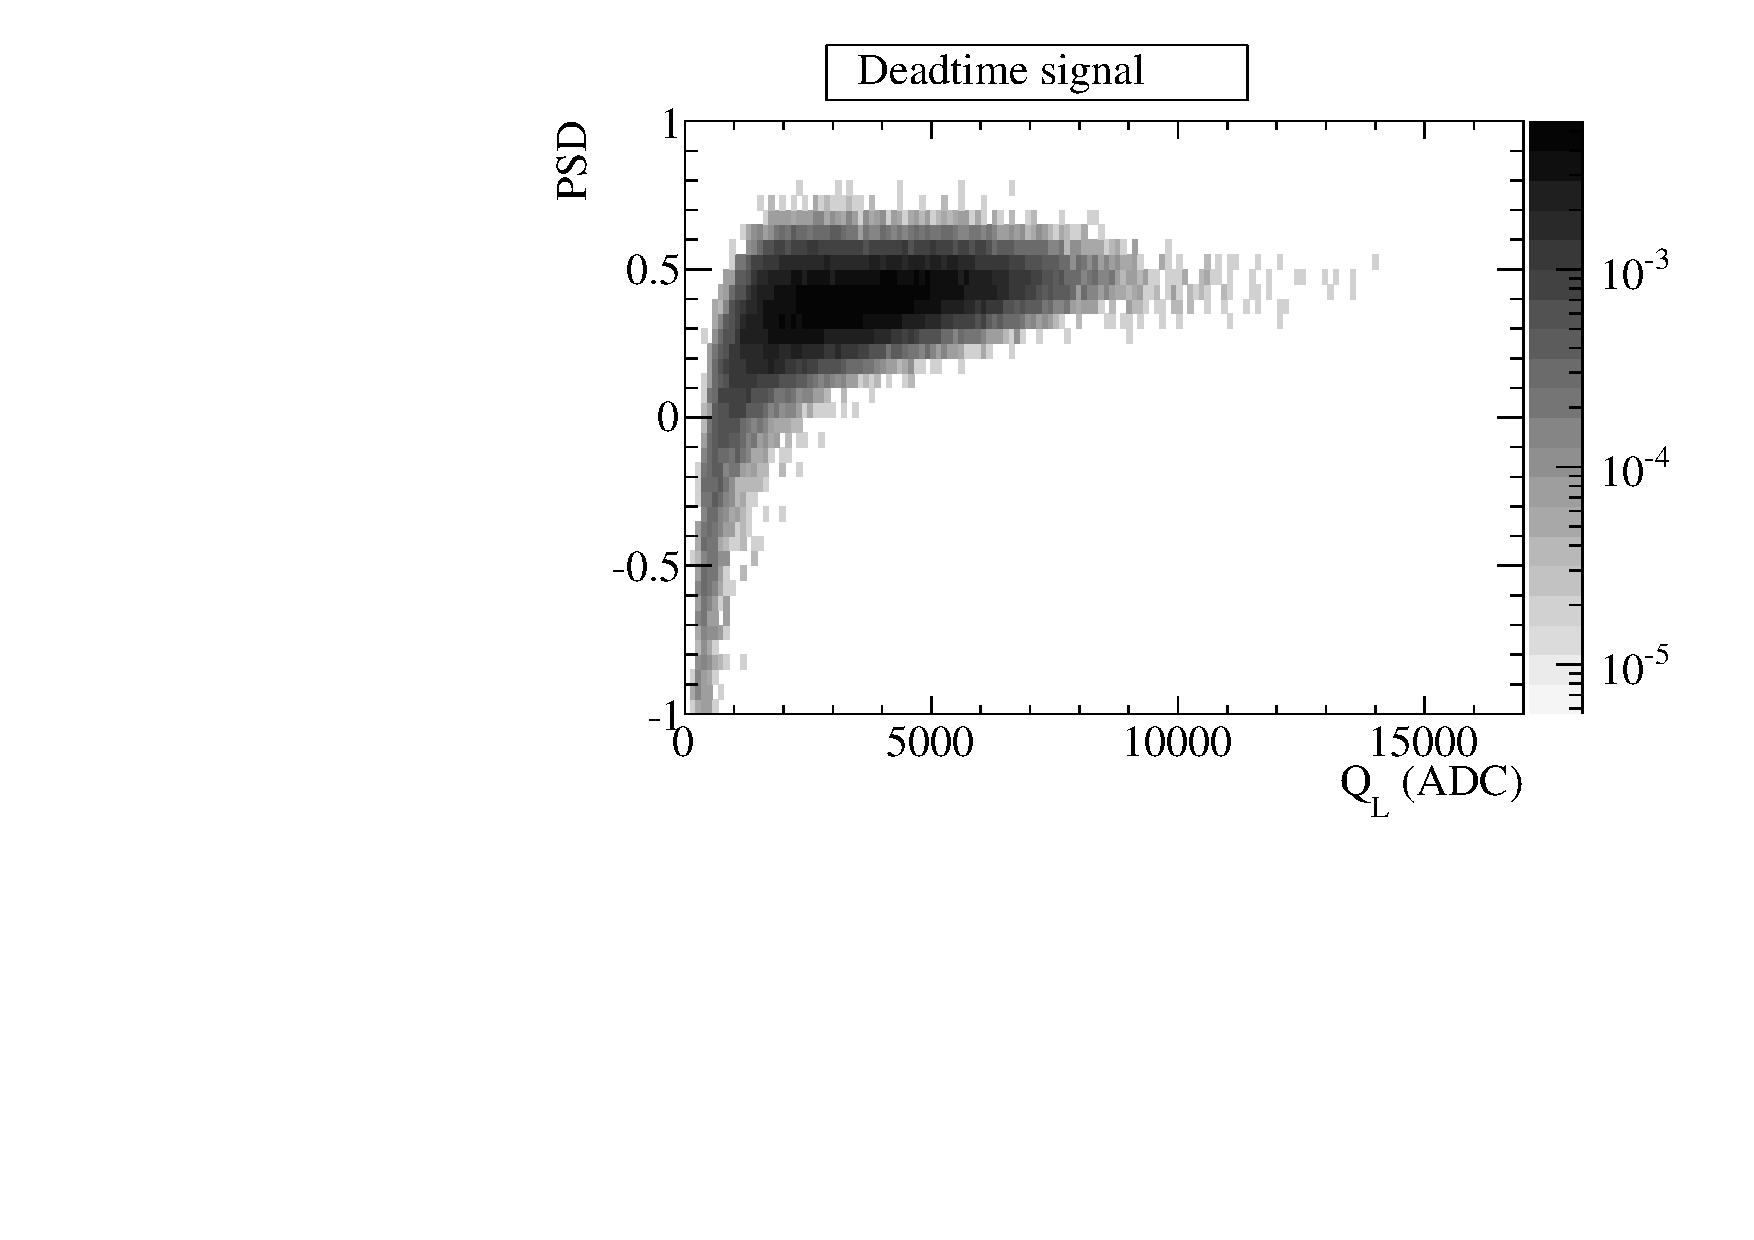
\includegraphics[width=0.45\textwidth]{figures/hlate_psdql.pdf}
\caption{ Event count (or relative event count) as a function of PSD
  and $Q_L$, going from top to bottom is for N background simulation,
  single neutron plus single background simulation, dead-time neutron
  simulation, and re-trigger on late light simulation.}
\label{fig:eventSpectra2}
\end{figure}


\section{Estimate of the absolute detector efficiency and background contamination}\label{sec:eff}

In order to determine the UCN detection efficiency of the $^{6}$Li the
active area of the detector, losses due to absorption in the front
face, and neutrons lost due to the background rejection cuts need to
be considered.  In principle one also has to take into account the
spectrum of UCN that are being detected.  Here we will assume that we
want to know the efficiency for detecting UCN with kinetic energy
above the effective Fermi potential of the GS30 lithium glass ($\sim$
$107$~neV).  Then if one has a known spectrum of UCN, the efficiency
for detecting could be estimated as zero for the UCN below 107~neV,
and the value we estimate here for those above 107~neV.  Note that the
Fermi potential of the GS20 (83~neV) is lower, so should have
negligible effect.


\subsection{ Detector effective area }

The estimate of the detector's effective area comes from a photograph
of the front face of the detector, where the side length of each of
the squares of $^6$Li glass is $29.0\pm0.1$~mm.  Using this known
length the pixels in the photograph that make up the circular aperture
of the detector are counted as the denominator, and the count of
pixels containing lithium glass as the numerator.  A photograph of the
detector face, that has been put in grey-scale, is shown in
Fig.~\ref{fig:detface}.  From this image the estimated active area of
the detector is $97.4\pm0.1$\% of the whole aperture.

\begin{figure}[!htpb]
\centering 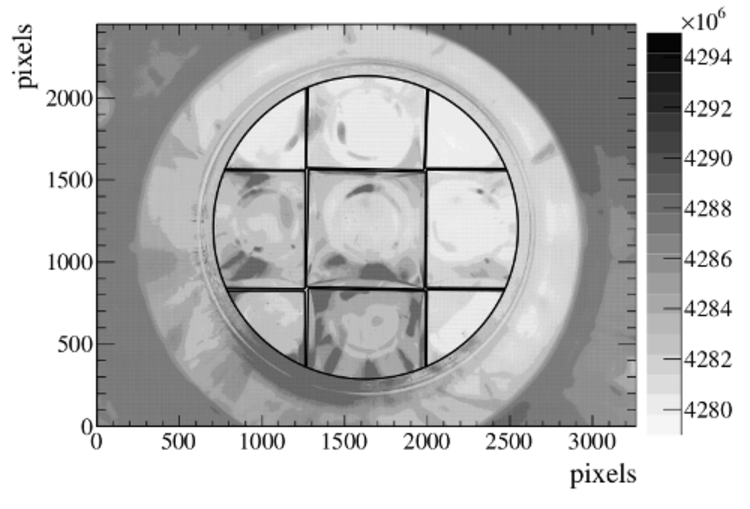
\includegraphics[width = 0.49\textwidth]{figures/detface.pdf}
\caption{Gray-scale image of the detector face used for estimating the
  areal efficiency of the detector.  The detector aperture and edges
  of the lithium glass are identified by the black lines.}
\label{fig:detface}
\end{figure}

\subsection{ Estimation of UCN absorption in Li depleted layer }

The cross section for absorption of UCN on $^{^6}$Li is $\sigma =
(4.5\pm2.5)\times10^{5}$~barns\cite{ban}.  The company contracted to
thin our samples of lithium glass has estimated our GS30 (lithium
glass depleted in $^6$Li) layer to be $(55\pm10)$~$\mu$m thick.  Given
that the lithium content in GS30 is $N = 2.4\times10^{-24}$~$cm^{-3}$,
the absorption length, $\lambda=1/(N\sigma)$, is
$\lambda=1.35\pm0.75$~cm.  The fraction of UCN making it through our
GS30 layer is calculated to be $99.34\pm0.43$~\%.

Measurements of the transmission of UCN through different thicknesses
of GS30 have been conducted by the PSI group at the Institut
Laue-Langevin in Grenoble\cite{Senoville}.  Using their measurements,
for a $55\pm10$~$\mu$m GS30 layer the UCN transmission is
$92.6^{+1.2}_{-1.8}$\%. The uncertainty is asymmetric due to the
exponential nature of the attenuation through a layer with uncertain
thickness.  The measurements suggest that the UCN loss through a GS30
layer is not dominated by the $^{6}$Li content, but by losses by
up-scattering on other material of the glass such as on Si and O.

\subsection{ PSD cut efficiency and background rejection}

The PSD and $Q_L$ cut efficiency for keeping UCN, and background
contamination remaining is estimated using an extended maximum
likelihood fit of the PDF templates described in
Section~\ref{sec:sim}.  The PDFs, binned in PSD and $Q_L$, are
labelled as $P_{i}( PSD, Q_L )$, where $i$=( 1 sig, N sig, 1 bg, N bg,
1 sig 1 bg, dead, or retrig).  The number of each type of event is
estimated as $N_i$ by minimizing a negative log likelihood that is
calculated as a sum over all $M$ of the PSD$^j$ and $Q_L^j$
measurements in the data as:

\begin{equation}
-\ln{(L)} = \sum_{i}^{7} N_i - \sum_{j}^{M} \ln{ \sum_{i}^{7} P_i( PSD^j, Q_L^j) }.
\end{equation}

A projection of the results onto the PSD and $Q_L$ axes for one of
these fits is shown in Fig.~\ref{fig:fits}.  All of the features seen
in the data are reproduced in the fit, although the reduced
chi-squared of the fit is rather poor.  We attribute the differences
to details that are not properly modelled, such as any contribution
from light leaks, PMT after-pulsing, and differences in gain variation
between the nine channels of the detector.

\begin{figure}[!htpb]
\centering 
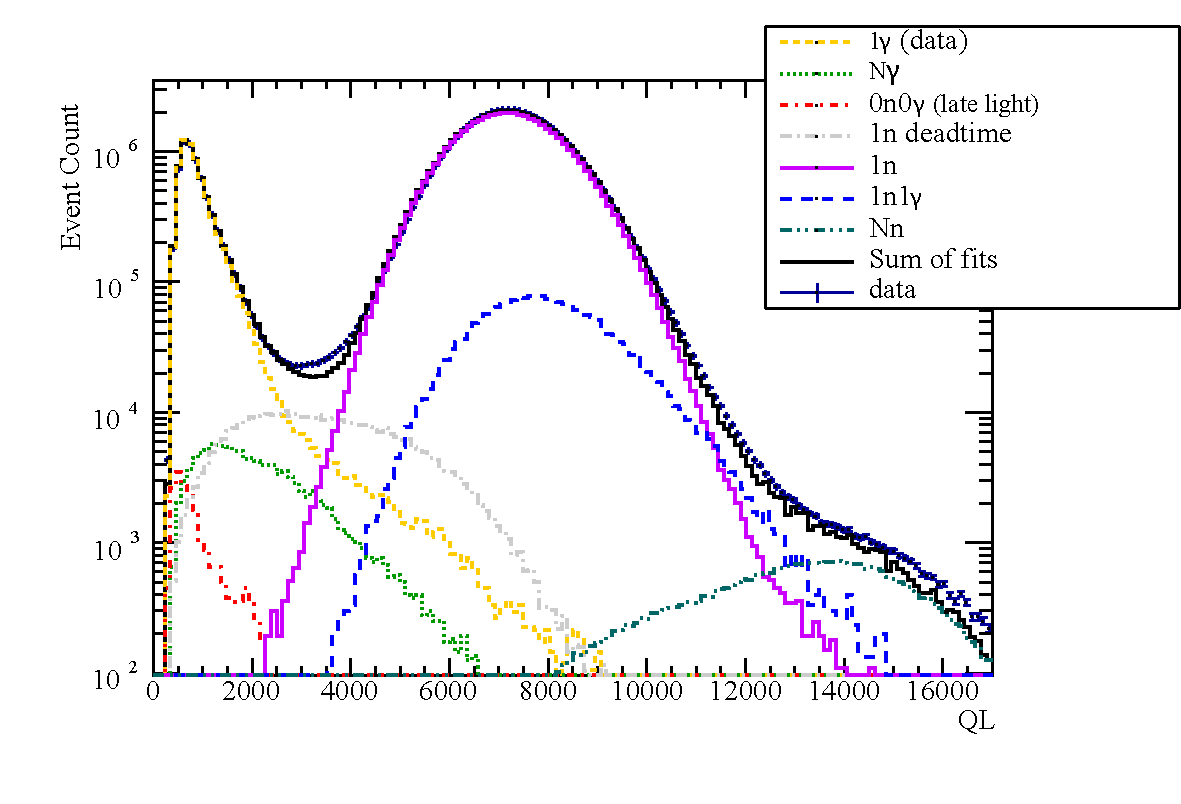
\includegraphics[width = 0.49\textwidth] {figures/qlfit.pdf} 
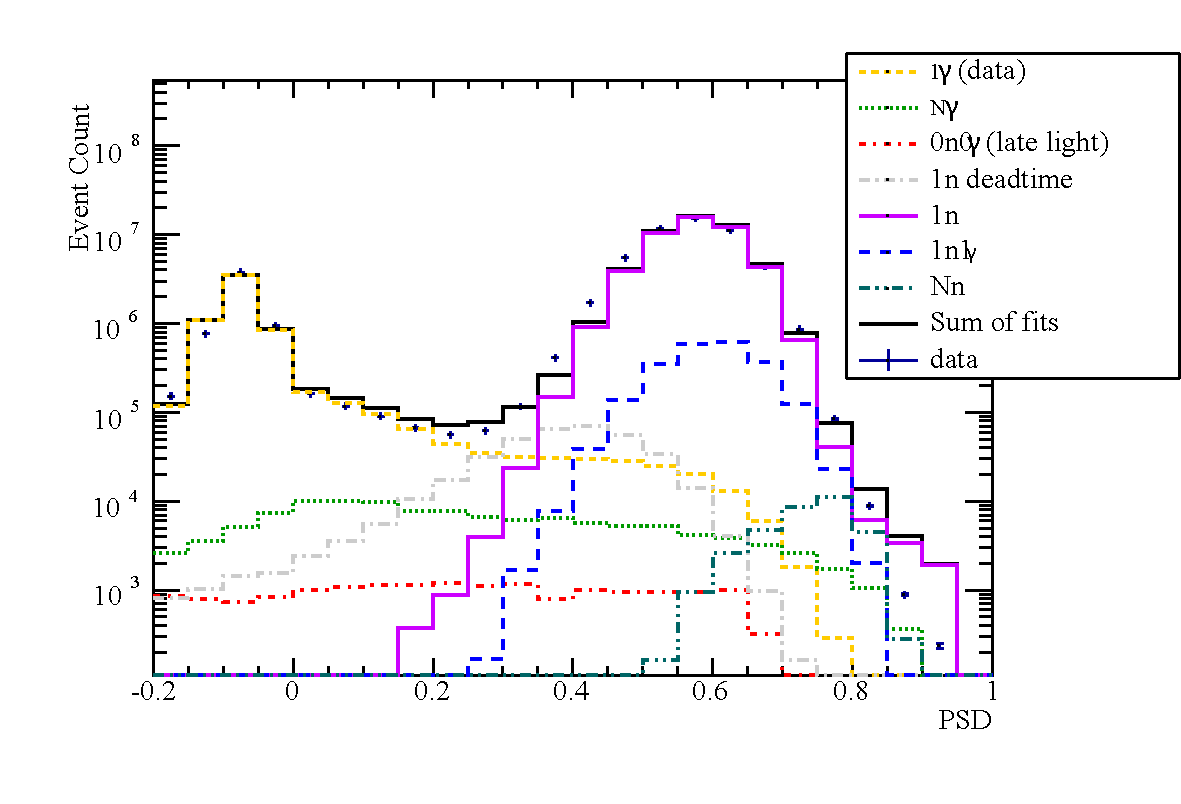
\includegraphics[width = 0.49\textwidth] {figures/psdfit.pdf}  
\caption{ Template fit results in the one dimensional projections
  along the total event charge (top) and along the PSD (bottom).}
\label{fig:fits}
\end{figure}


\paragraph{Cut detection efficiency and background rejection estimates}

Using the template fit, the neutron detection efficiency and
background contamination are computed for different cut values in PSD
and $Q_L$.  The signal templates, in addition to single neutrons (1n),
are taken to include multiple neutrons (Nn), dead-time neutrons (1n
deadtime) and single neutron single gamma (1n1$\gamma$) events.  The
background rates are extracted from the single gamma (1$\gamma$), late
light (0n0$\gamma$), and multiple gamma (N$\gamma$) templates.  If the
total number of neutrons in the templates is $N_n$, and the number of
neutrons above a given cut value is $N_n^{cut}$, then the neutron
efficiency due to background rejection cuts is defined as:

\begin{equation}
\epsilon_n = \frac{N_n^{cut}}{N_n}.
\end{equation}

\noindent If the number of events in the background templates above a
given cut value is $N_{\gamma}^{cut}$, then the background
contamination fraction is defined as:

\begin{equation}
\eta_{\gamma}= \frac{N_{\gamma}^{cut}}{N_n},
\end{equation}

\noindent and the background rejection as:

\begin{equation}
\epsilon_{\gamma} = 1 - \eta_{\gamma}.
\end{equation}

\noindent Figure \ref{fig:detectionEff} shows the neutron efficiency
and background contamination of the entire beam pulse spectrum for two
PSD cuts.  For a cut $Q_L>3000$~ADC and PSD$>0.3$, the neutron
acceptance is $99.5\pm0.5$\% and the background contamination
is $0.3\pm0.1$\%.

%paragraph illustrating possible systematics from this

\begin{figure}[!htpb]
\centering 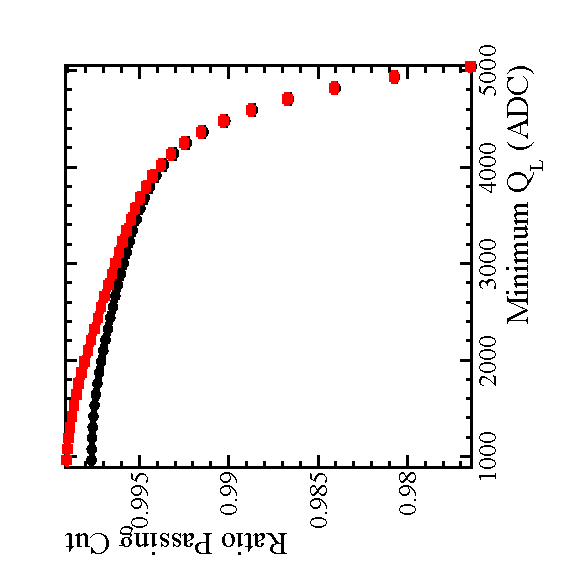
\includegraphics[width =0.49\textwidth, angle=-90]{figures/neutroneff.pdf}
\centering 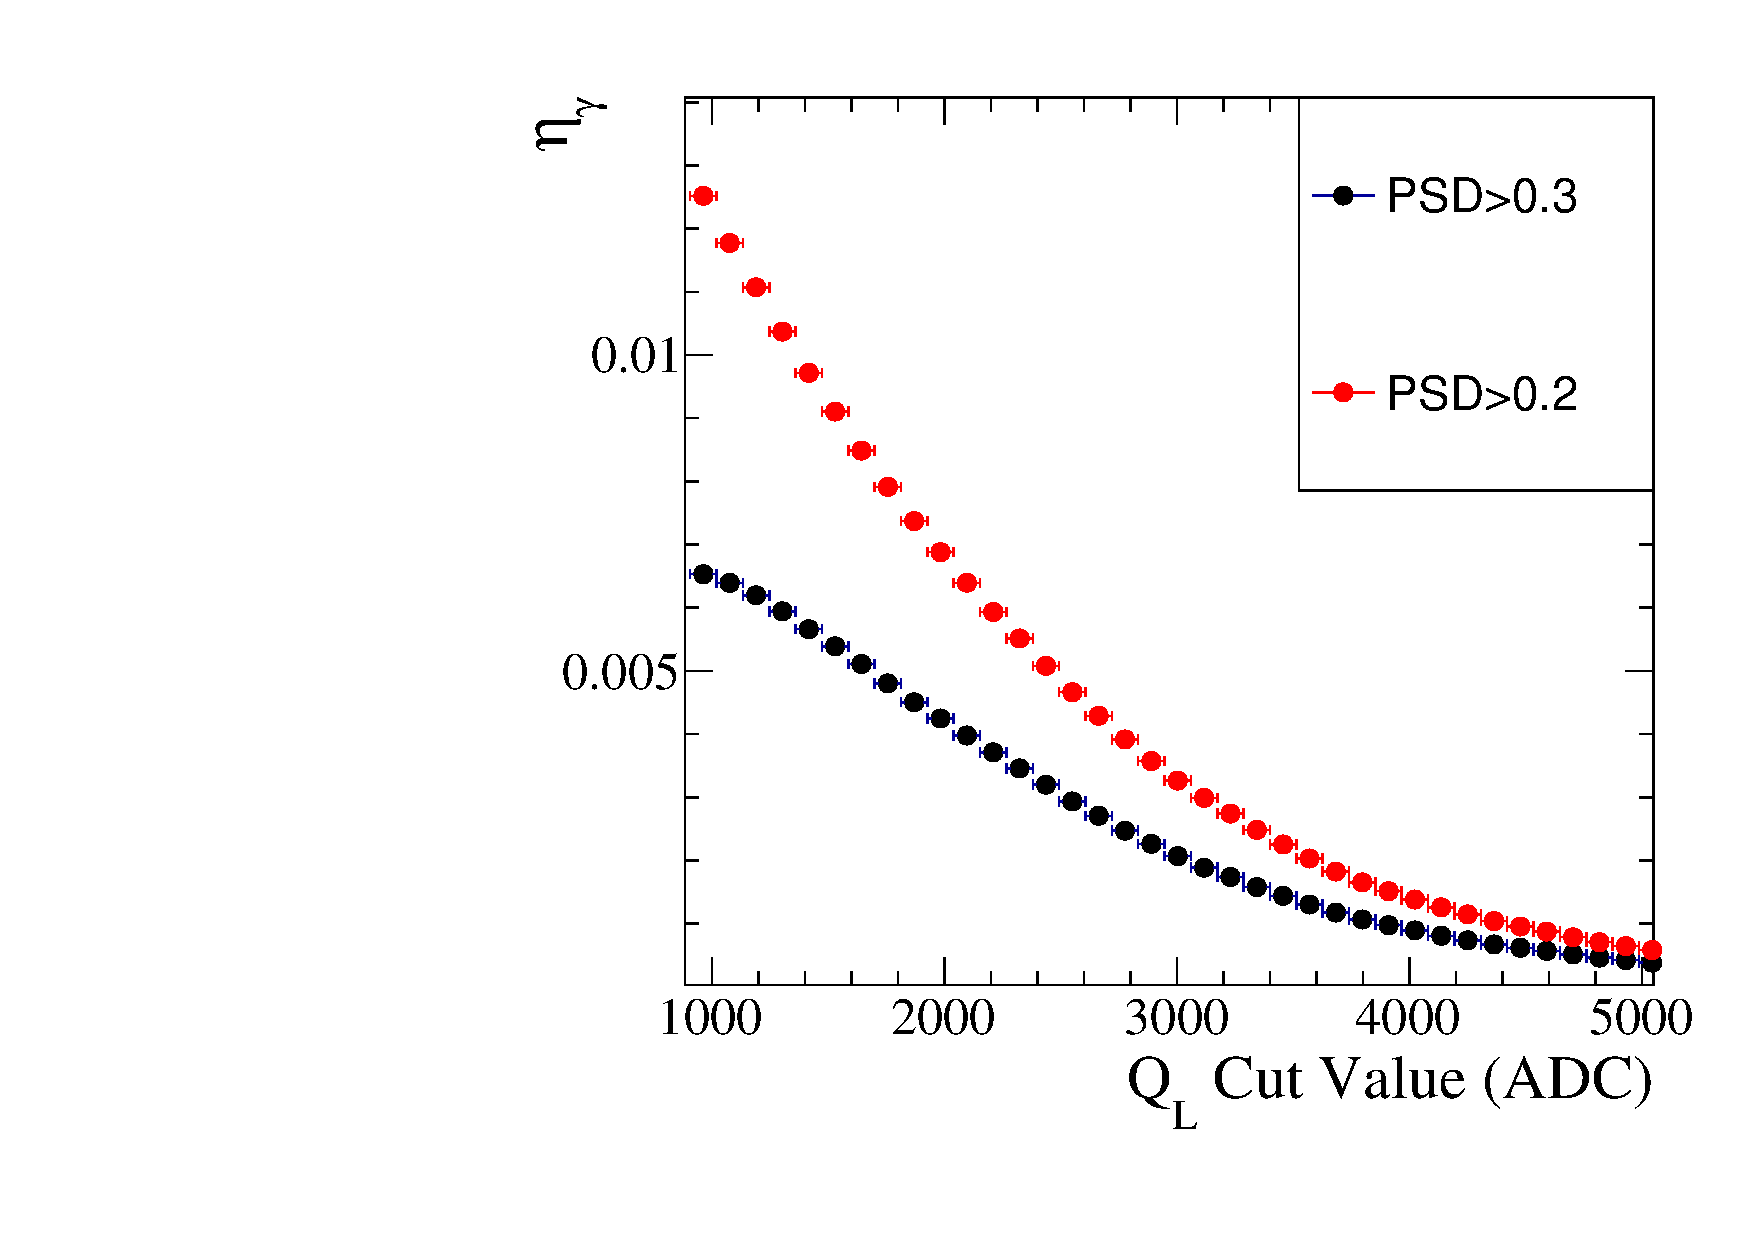
\includegraphics[width =0.49\textwidth, angle=-90]{figures/backgroundconta.pdf}
\caption{ Neutron cut efficiency (top panel) and background
  contamination (bottom panel) for different cuts on $Q_L$.  The red
  squares are with cut on PSD$>0.2$, and the black circles are for a
  cut on PSD$>0.3$ }
\label{fig:detectionEff}
\end{figure}

The rate of neutrons varies over the 300 second cycle of the UCN
produced at PSI.  To study the neutron detection efficiency and
background contamination at different rates, the data was split into
three time periods after the proton beam irradiation: high rate,
middle rate, and low rate.  The split data was fitted according to the
template fit and then the efficiency was calculated according to each
fit.  The low rate data had more background contamination than the
other rates, presumably due to the higher ratio of background to
signal events.  Using a cut on $Q_L > 3000$~ADC and $PSD>0.3$, the
neutron efficiency was $99.5\pm0.5$\% and the background contamination
was $0.3\pm0.1$\%.

\begin{figure}[!htpb]
\centering 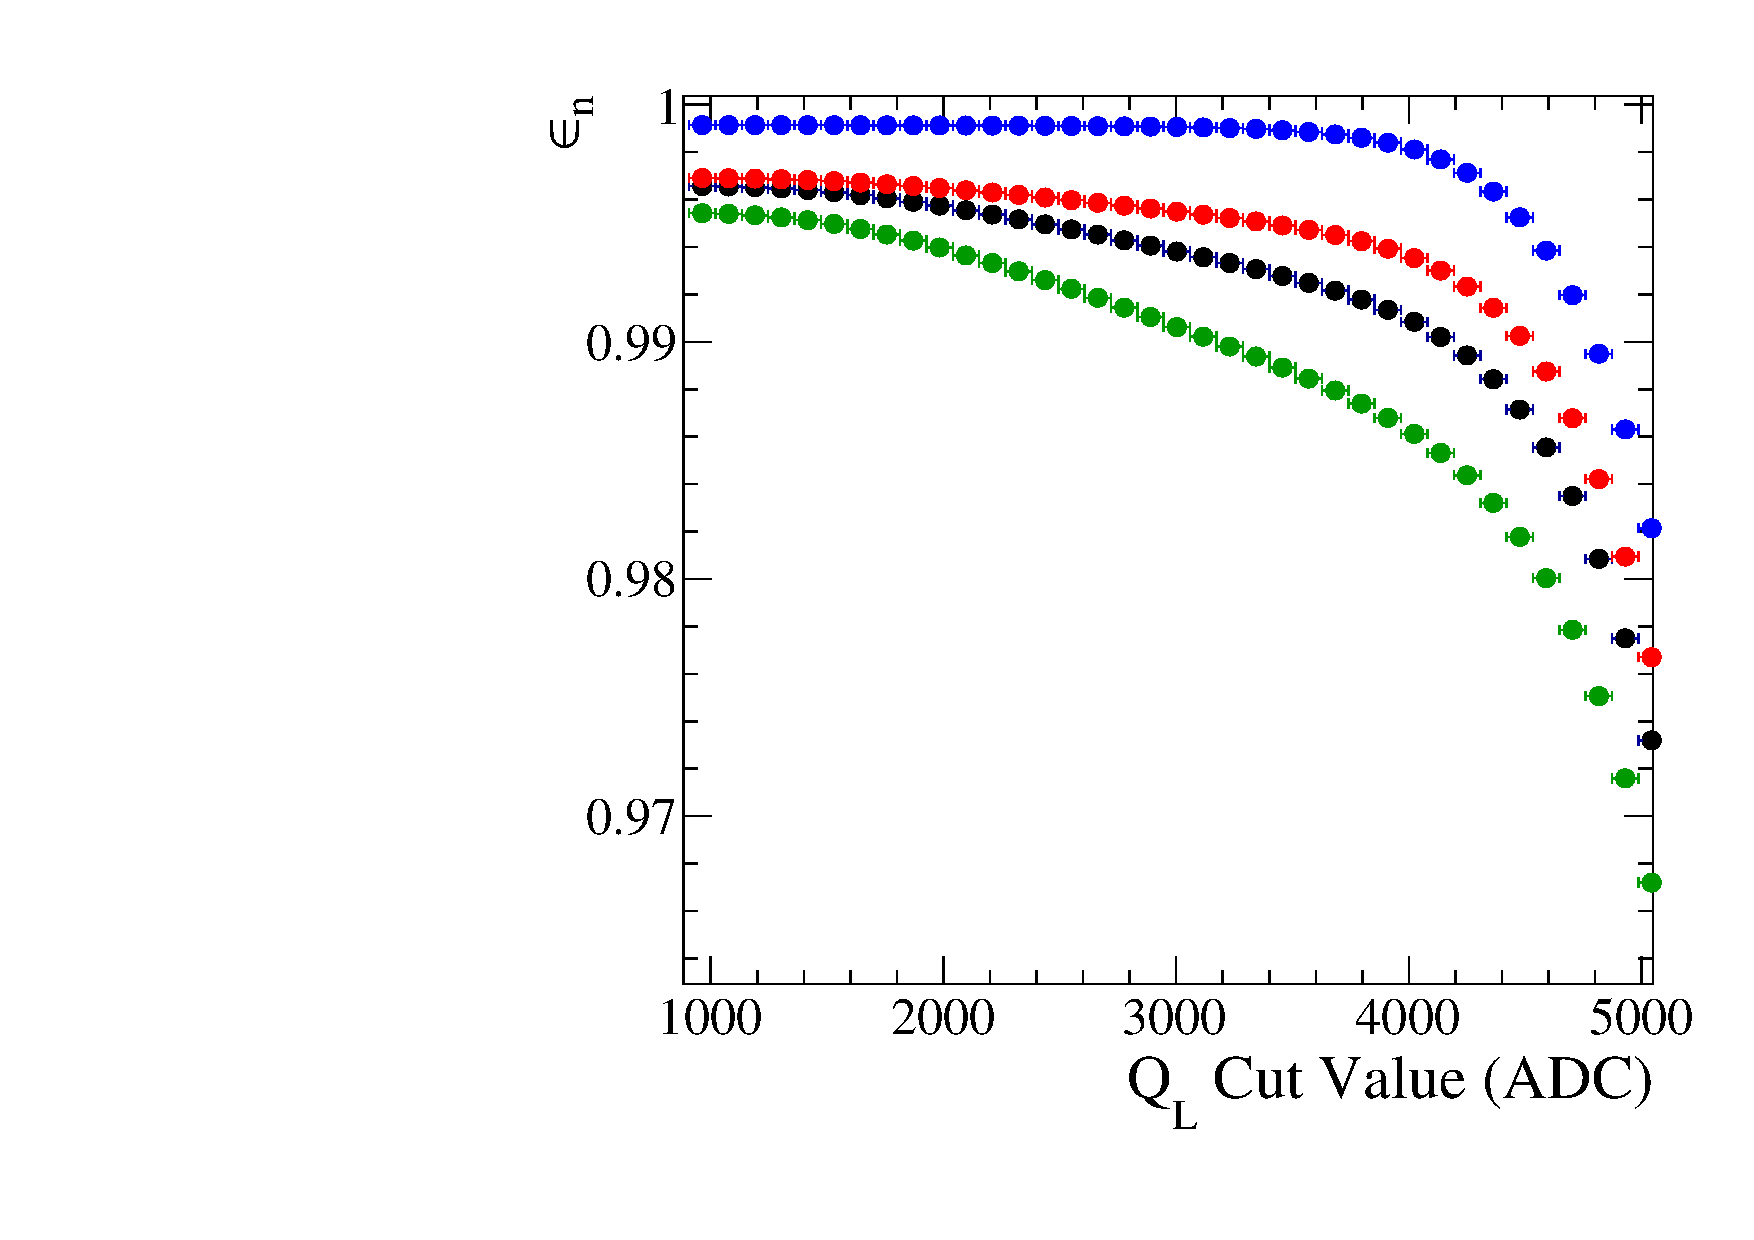
\includegraphics[width = 0.49\textwidth, angle=-90]{figures/neutronEffLayered.pdf}
\centering 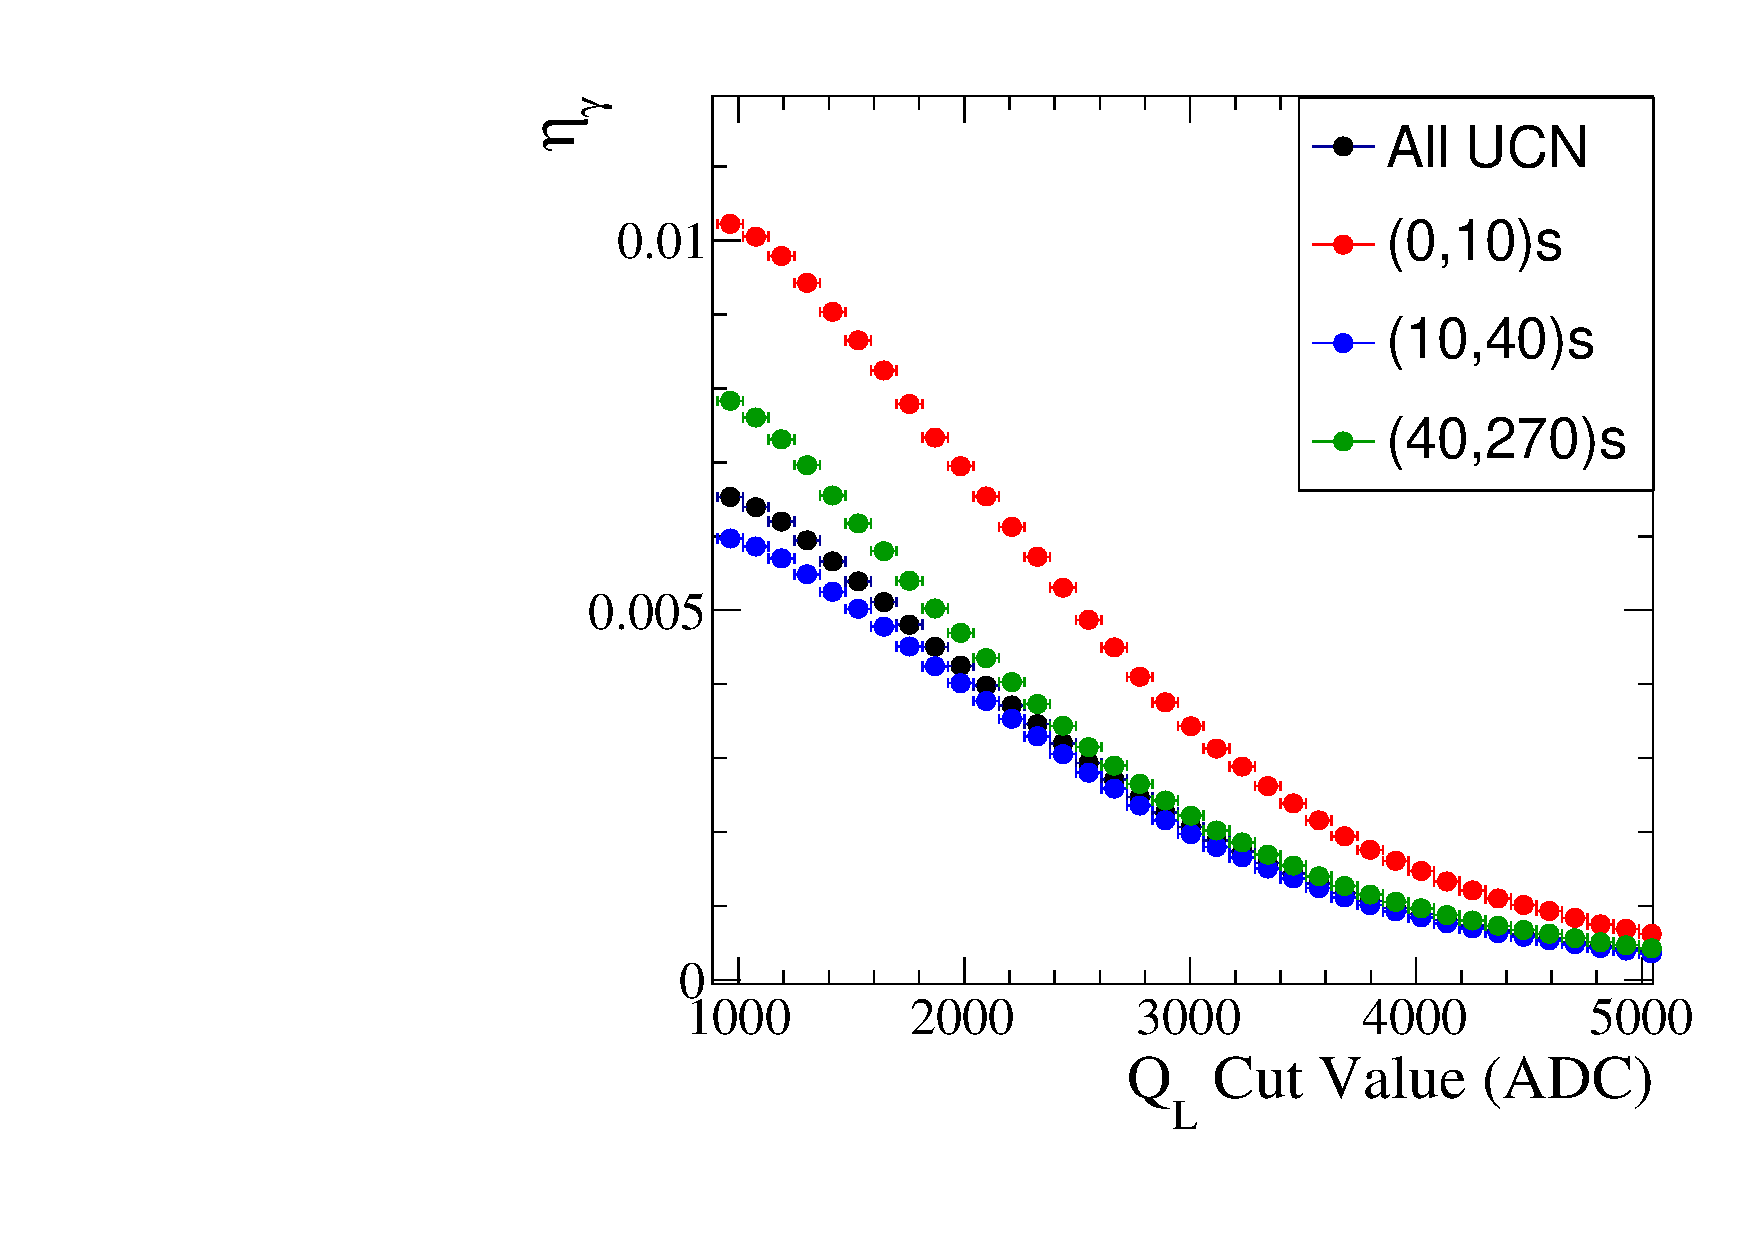
\includegraphics[width = 0.49\textwidth, angle=-90]{figures/backgroundContLayered.pdf}
\caption{ Neutron cut efficiency (top panel) and background
  contamination (bottom panel) for different times since the UCN
  production.  The red boxes are for an average UCN rate of $>$~70~kHz
  over the first 10~s of UCN, the blue downward-triangles are for an
  average UCN rate of $>$~20~kHz over the next 30~s, and the green
  upward-triangles are for an average rate of $<10$~kHz over the last
  230~s.}
\label{fig:detectionEffLayered}
\end{figure}

The $^6$Li detector therefore has a very good background rejection due
to the signal shape variation between lightguide background and the
scintillation events from the lithium glass.

\subsection{Overall Detector Efficiency Estimate}

The overall detection efficiency, for the rates of UCN at PSI,
including all of the effects described in this section, is
$89.7^{+1.3}_{-1.9}$\%, which is dominated by the uncertainty in the
absorption in the GS30 layer. The rate dependence of the efficiency is
below the $0.5$\% level.  This uncertainty could be improved by
applying what we know about the statistics of random signals and
backgrounds to model the expected rates.  This would represent an
improvement to the simple fit with unconstrained fractions of
different types of pile-up described in this paper.


\section{ Relative rate comparison }\label{sec:relative}

We used the two beamlines called ``West-1'' and ``West-2'' at the PSI
UCN source\cite{ucnBeam}.  West-2, described in more detail in
reference \cite{ucnBeam}, offers the distinct feature that UCN have a
dropping height of minimum 120~cm before reaching the detector.
West-1 in a horizontal configuration provides UCN with energies
starting above 54~neV given by the safety AlMg$_3$ foil in the
beamline.  

UCN rates on the West-1 beamline are typically a factor of
10 higher than on West-2.  The operation mode during our measurements
was however given by the priority of the nEDM experiment measuring at
the third beam-port.  During the measurement period described here, the
UCN source operation was using 3 second long proton beam bunches with
a repeating period of 300 seconds .  During and after the proton beam
bunches the UCN can propagate down the beam line to the experiment
area.  Typical UCN detector rates during 300 second periods in West-1
and West-2 measured with our scintillation detector are shown in
Fig.~\ref{fig:protonCycle}.  

Note that our detector's 75~mm diameter
aperture does not match the 160~mm aperture of the West-1 beam-line,
and that it can only see UCN above the Fermi potential of the
scintillating glass (107 neV).  This means that we see relatively
more UCN from the vertical source, that has a spectrum starting at
about 100~neV, matching our detector Fermi potential, than from the
softer source of the horizontal West-1 beam.  The PSI group has made
measurements showing that on West-1, about 32\% of the UCN are between
54~neV and 100~neV.  Also two UCN cycles shown in the figure were
taken on different days, and we know from measurements of the PSI
group that during that time, the PSI UCN source saw about a 15\%
decrease in the number of UCN.  Therefore we expect to see less than
the 10$\times$ difference in UCN rate when comparing the distributions
in Fig.~\ref{fig:protonCycle}.

\begin{figure}[htpb] 
\begin{center} 
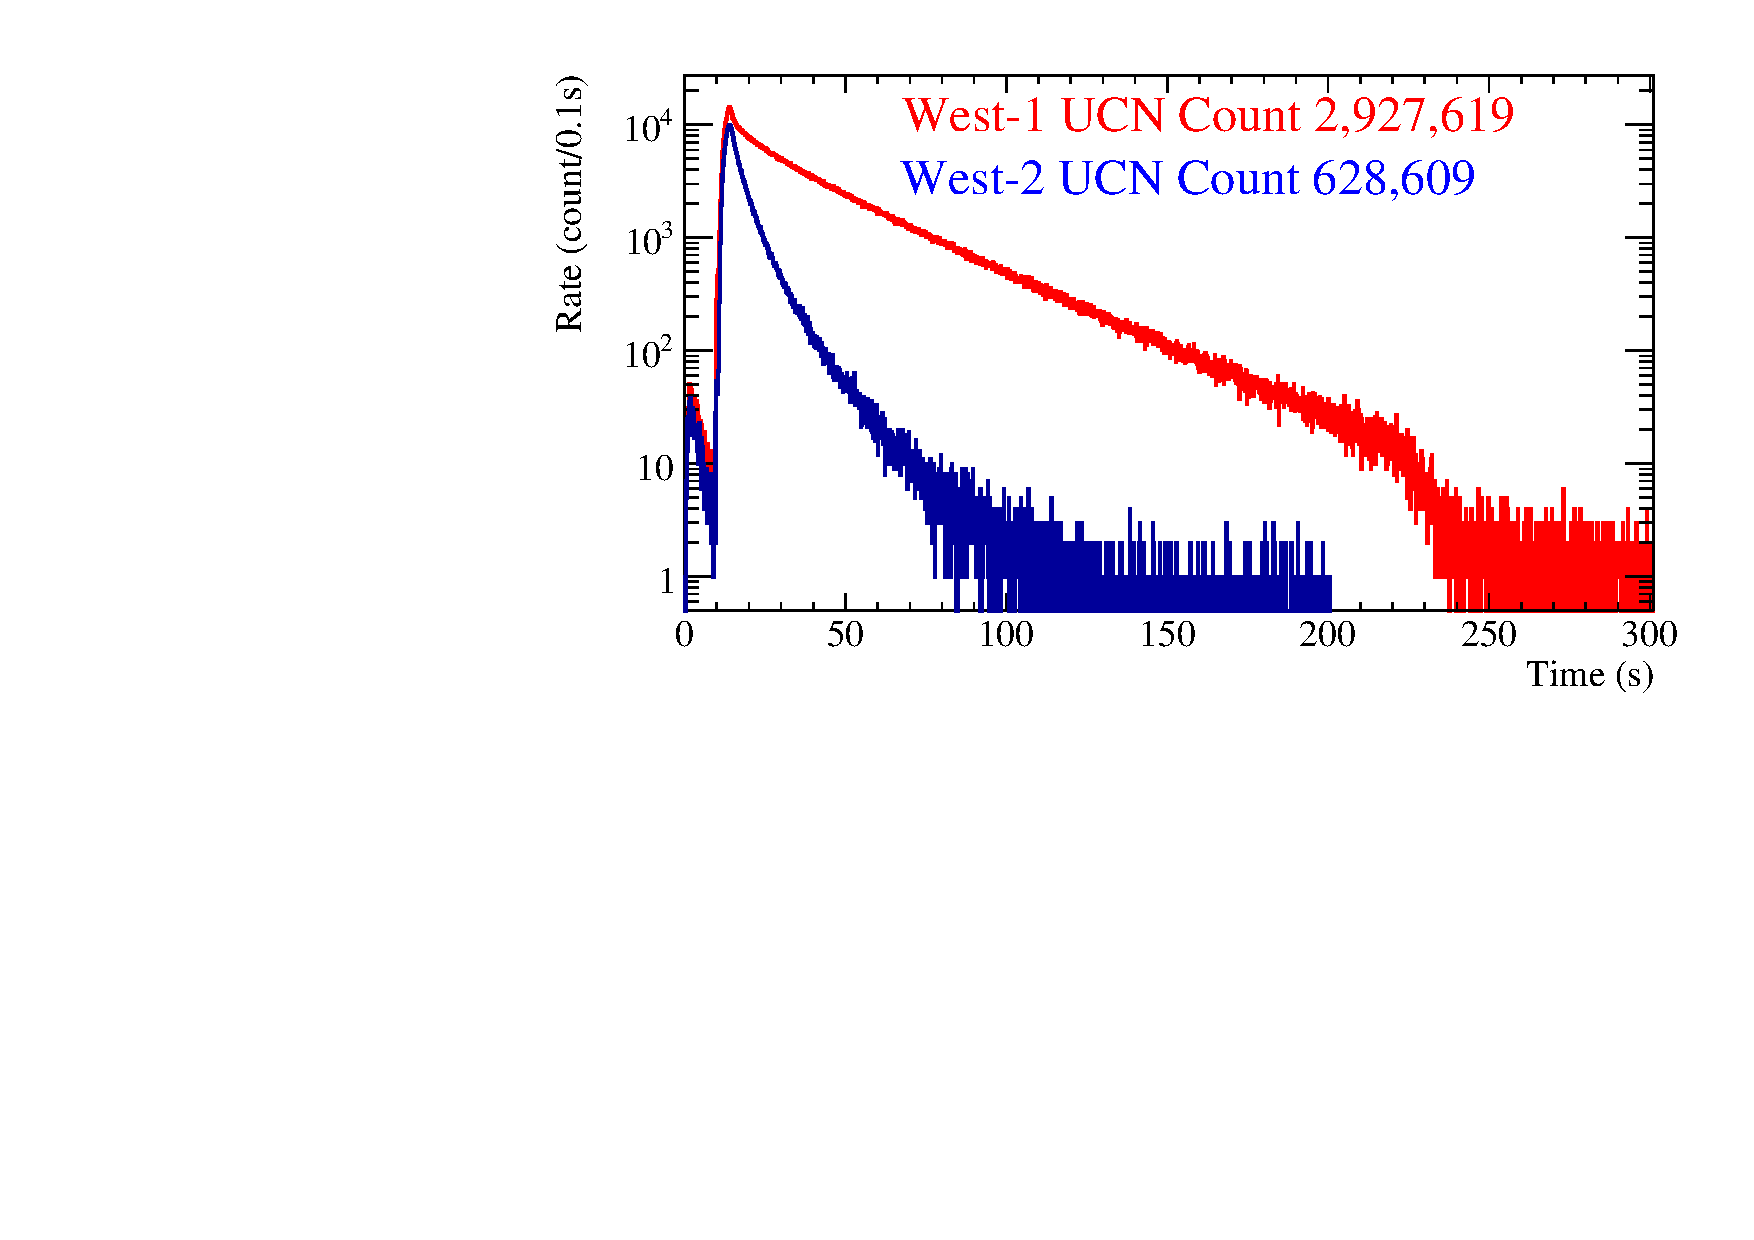
\includegraphics[width=0.49\textwidth]{figures/run54_to_run40_bunch0_compare.pdf} 
\caption{ UCN observed during one proton beam bunch, as detected with
  the Winnipeg $^6$Li UCN detector on West-1 (red) and West-2 (blue).
  The small peak before the main peak is caused by a 7~ms long pilot
  proton beam bunch used for checking the beam centering before the
  main beam bunch on the spallation target. }
\label{fig:protonCycle} 
\end{center} 
\end{figure}

The $Q_L$ distribution from each of the nine channels of the detector,
with a PSD cut at 0.3 to eliminate the lightguide backgrounds, is
shown in Fig.~\ref{fig:nineup}.  These data are from twelve UCN cycles
of the PSI source collected from the horizontal West-2 beamline.  It
is clear from these distributions that there is very little background
remaining.  The different numbers of counts seen make sense due to the
geometry of the detector.  The corner square tiles are shadowed the
most by the round aperture of the detector opening, giving them the
lowest count.

\begin{figure*}[!htpb]
\centering
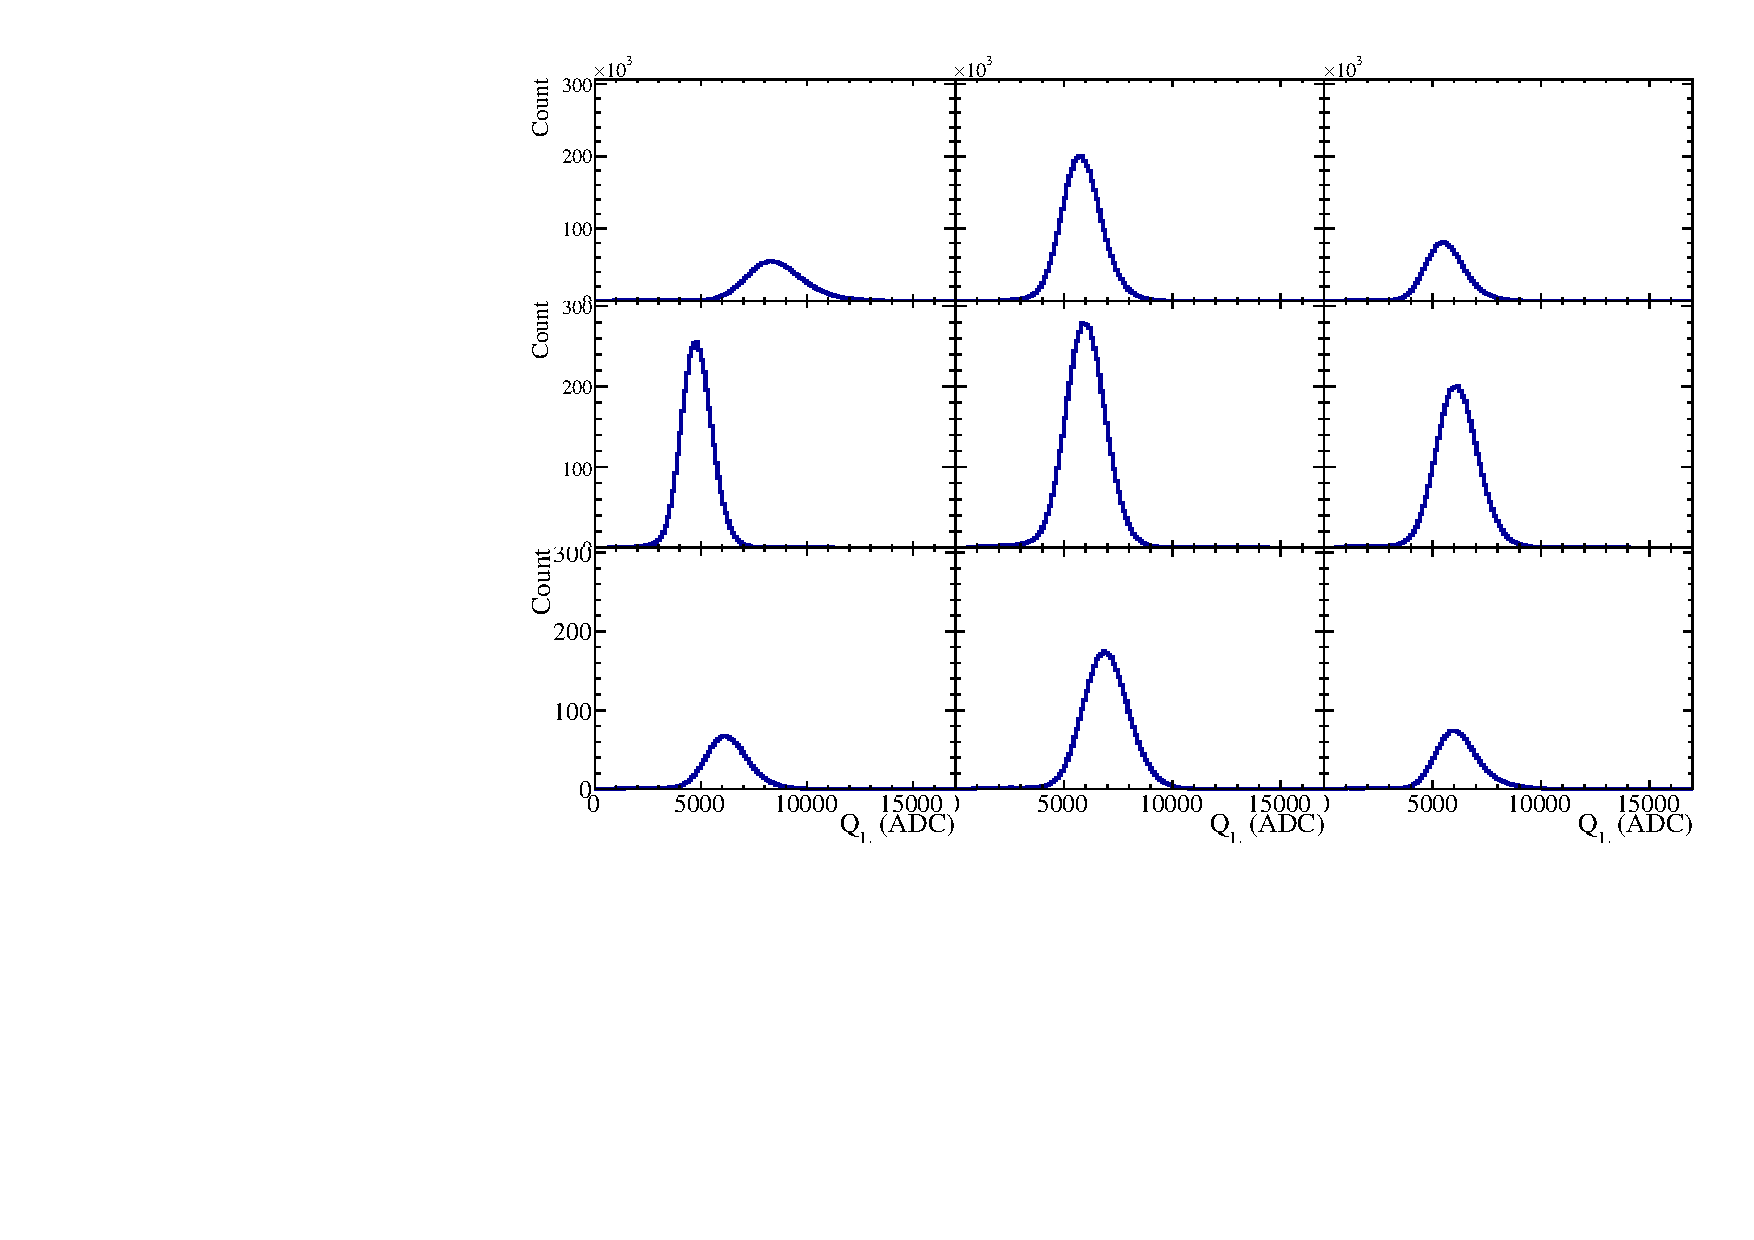
\includegraphics[width=0.95\textwidth]{figures/nineup.pdf}
\caption{ Event count per $Q_L$ bin from each of the nine channels of
  the $^{6}$Li scintillation detector from twelve cycles of UCN beam
  on the horizontal PSI West-2 beamline.}
\label{fig:nineup}
\end{figure*}


\subsection{ Channel to channel comparisons }

In order to determine the rate stability of the detector, the first
five channels' count (set A) per UCN cycle was compared to the last
four channels (set B).  During each UCN cycle on the West-2 beamline,
the $^6$Li detector counted about $3\times10^6$ neutrons, which has a
statistical uncertainty of 0.06\% (or 0.08\% in each of two equal
sized samples).  A long overnight run containing 114 UCN cycles (9.5
hours) was taken to assess the rate stability.  The count for each UCN
cycle in each set of channels, and the ratio of counts per UCN cycle
in set B over set A, is shown in Fig.~\ref{fig:ratiocount}.  Note that
there are four UCN cycles where the PSI nEDM experiment did not take
the UCN, and the number of UCN seen by our $^6$Li detector is higher
than all of the rest of the cycles.  Fitting the ratio of count rates
to a constant yields an acceptable $\chi^2$ per degree of freedom of
116.8 over 113, indicating that over the 9.5 hour data collection, the
counts seen in these groups of the channels, relative to one another,
is stable at the 0.08\% level.

\begin{figure}[!htpb]
\centering
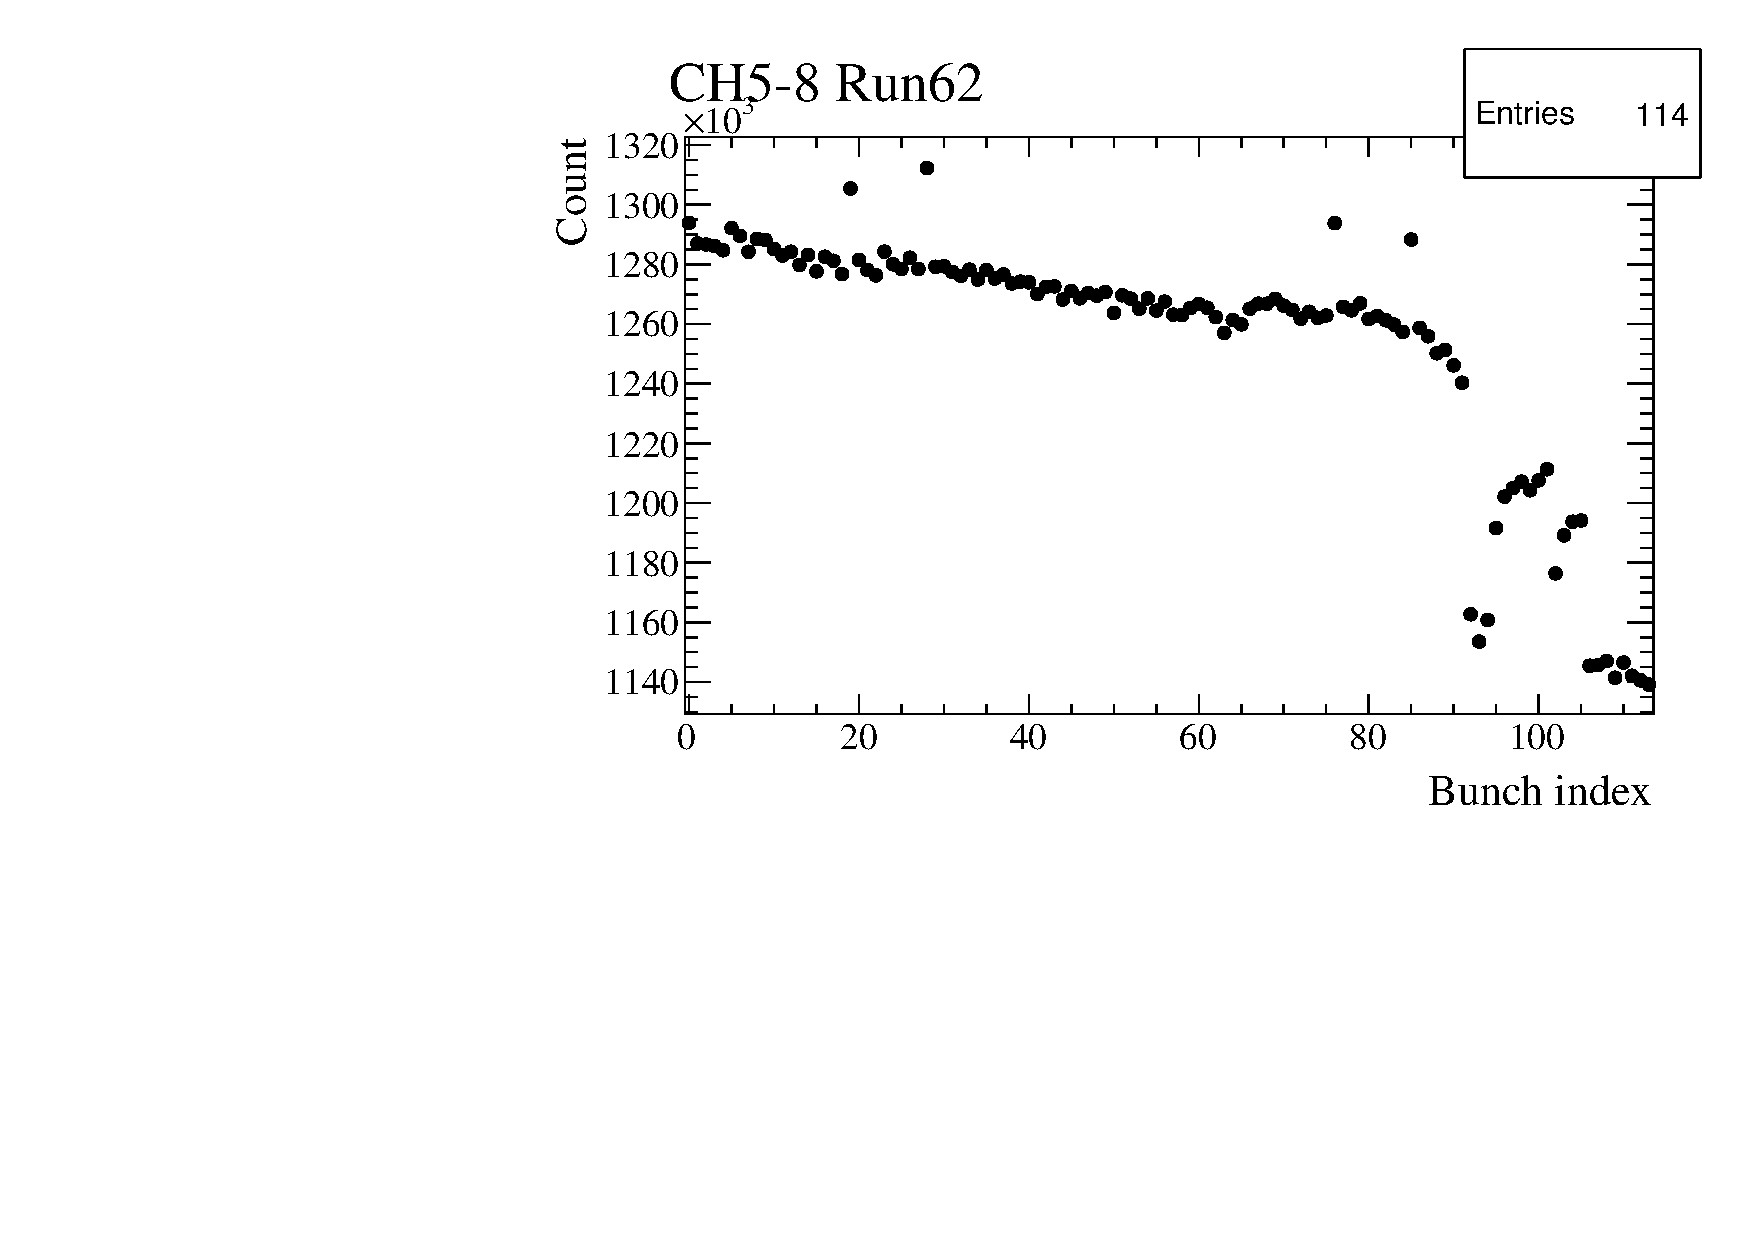
\includegraphics[width=0.45\textwidth]{figures/ratestab_ch04_Run62.pdf}
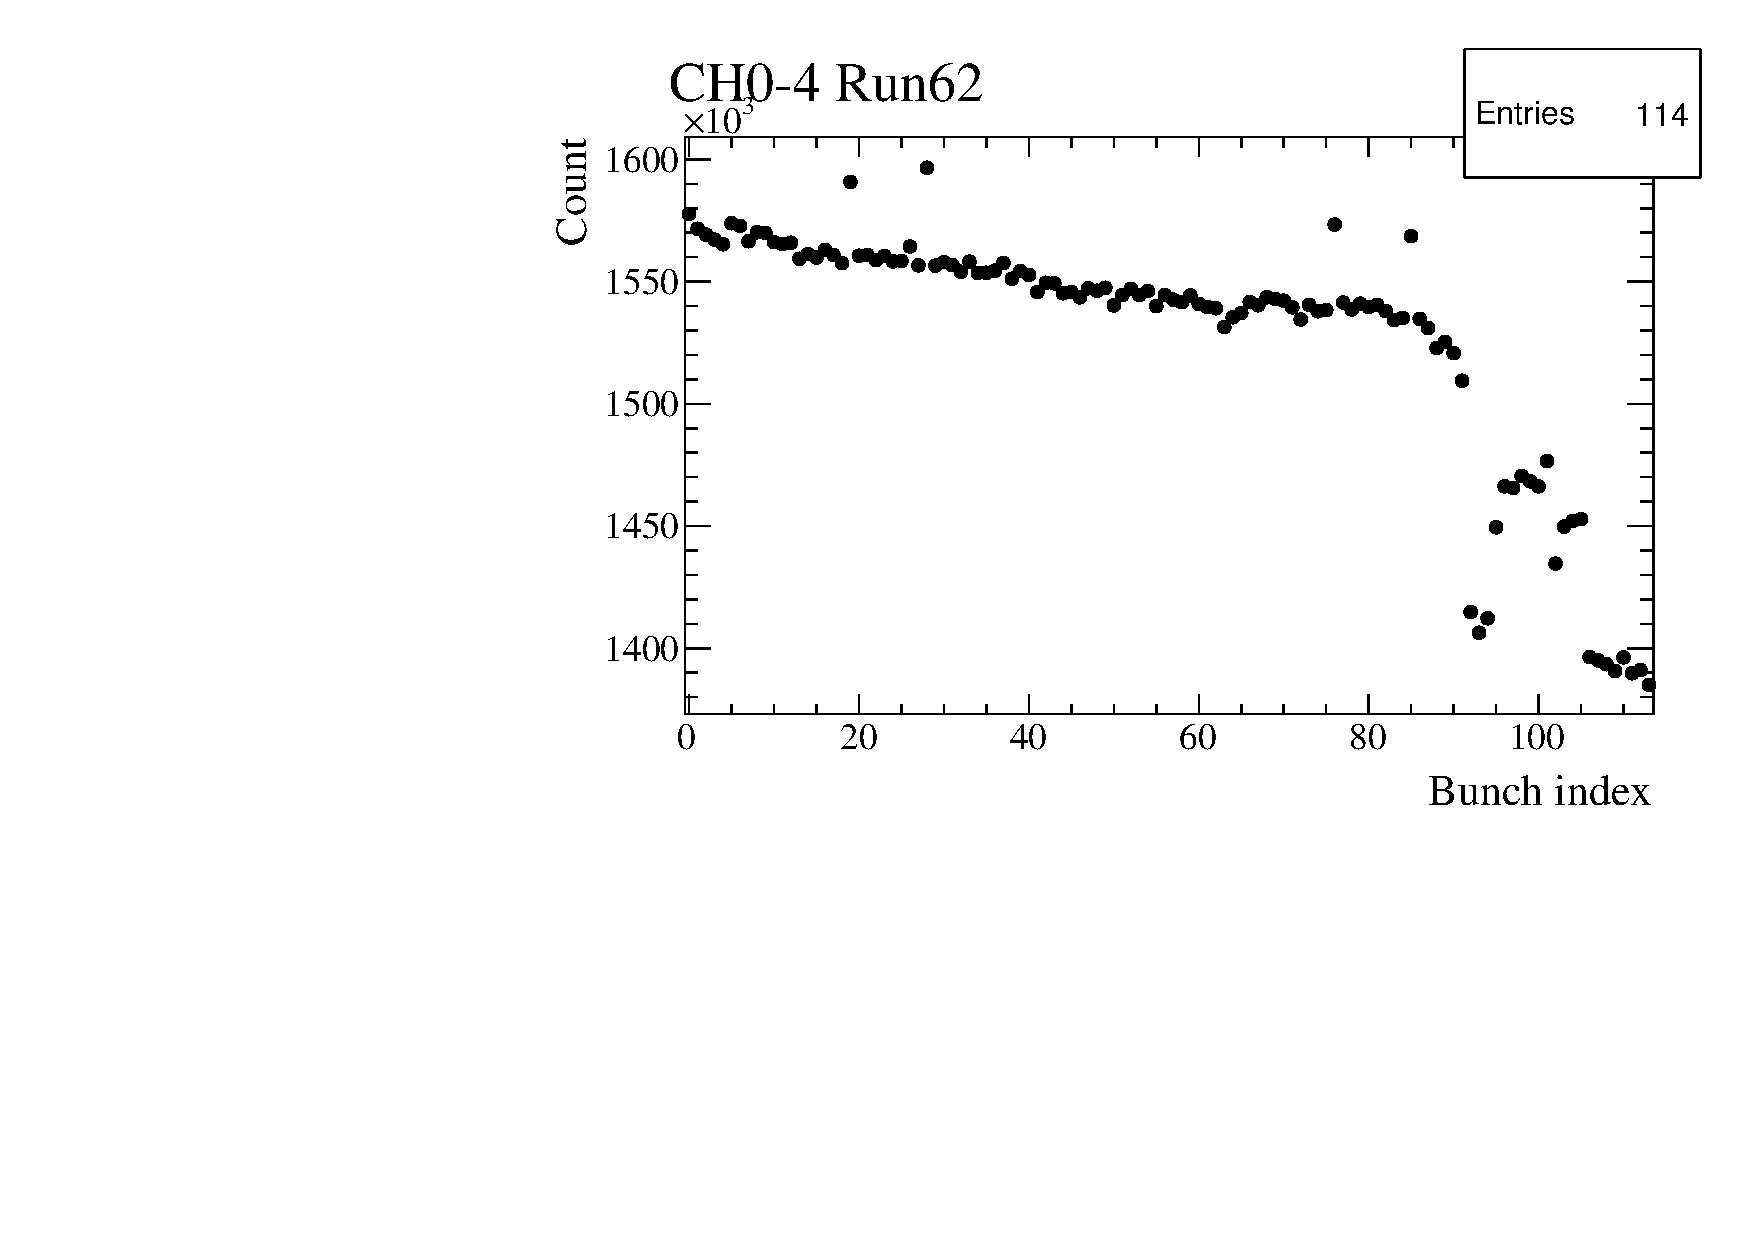
\includegraphics[width=0.45\textwidth]{figures/ratestab_ch58_Run62.pdf}
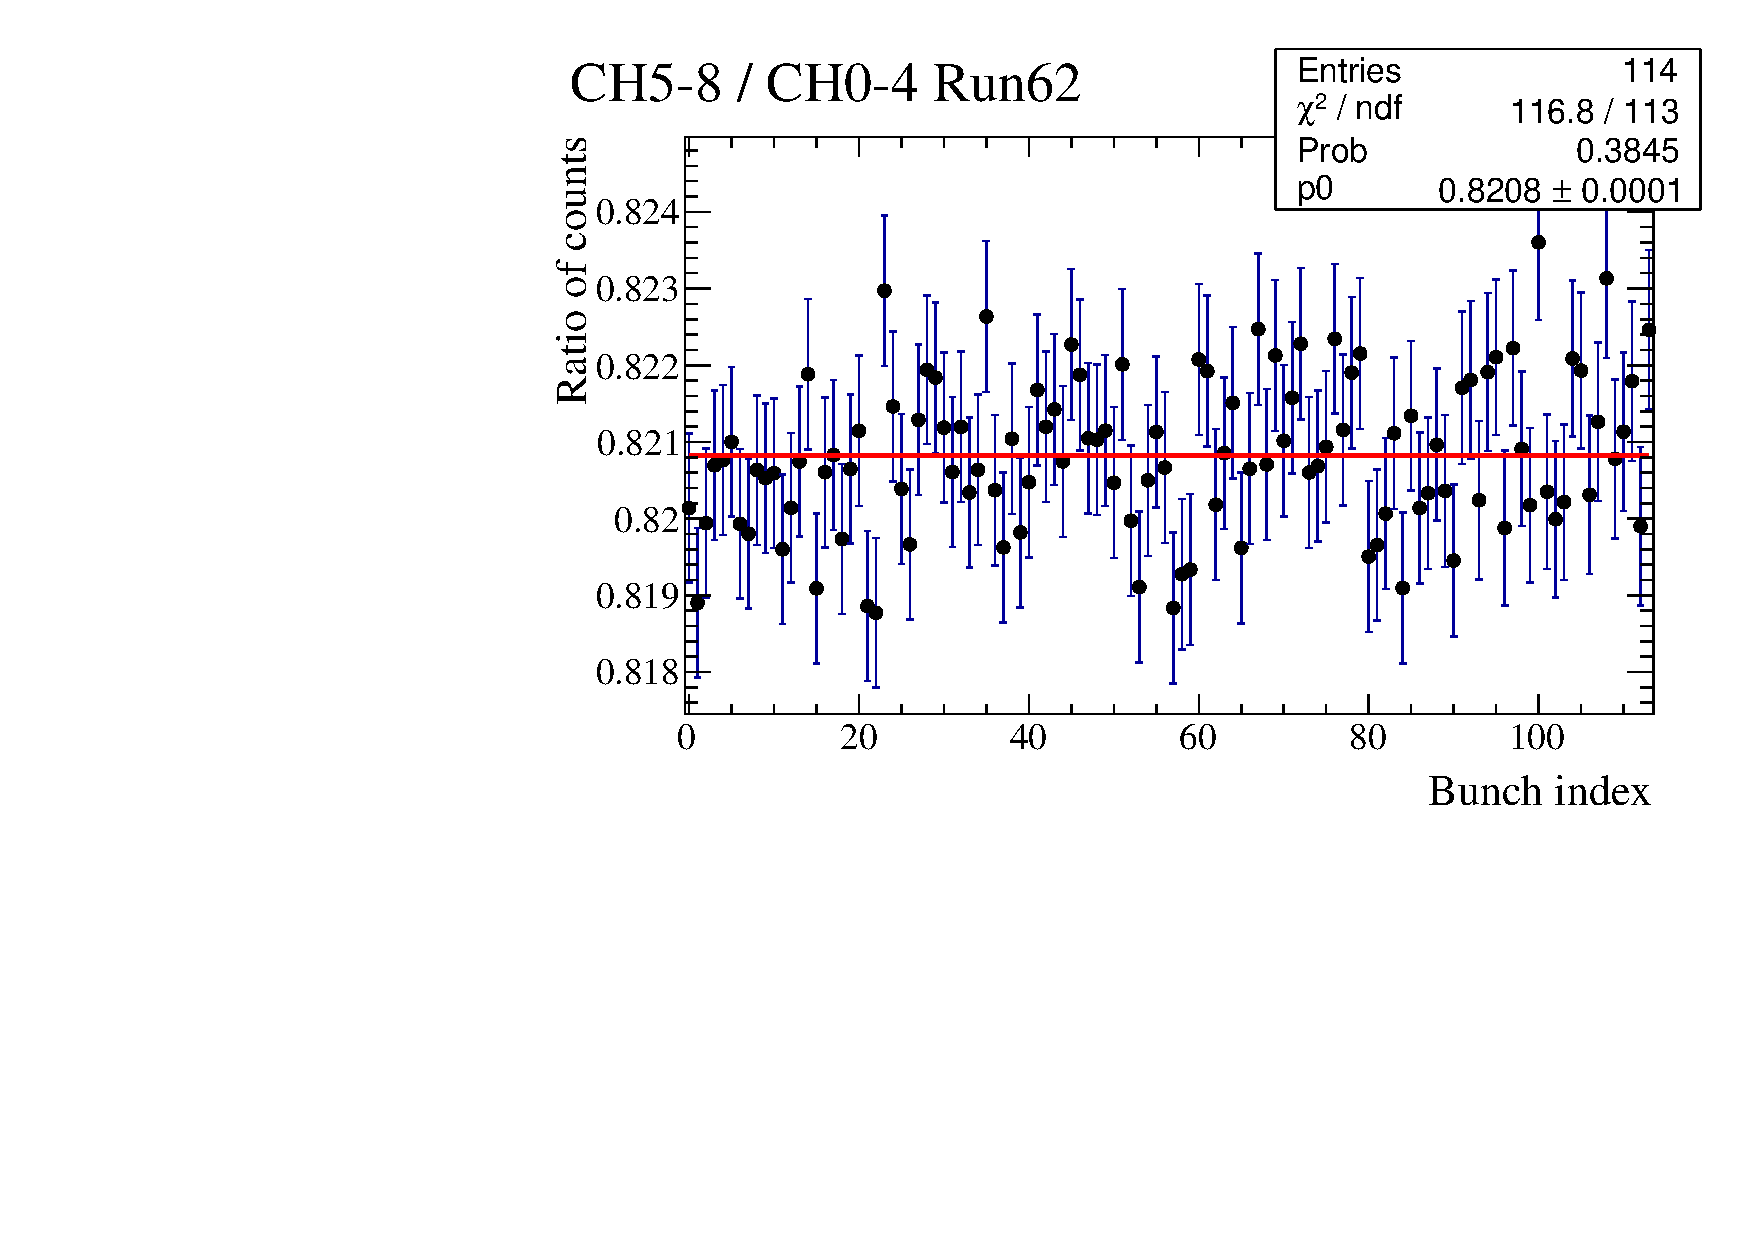
\includegraphics[width=0.45\textwidth]{figures/ratestab_ratio_Run62.pdf}
\caption{ The top panel shows the Event count from Set A (Channels
  0-4) for each of the 300 s UCN cycles on West-2, the middle panel
  shows the Event count from Set B (Channels 5-8), and the bottom
  panel shows the ratio of counts from set B over set A.}
\label{fig:ratiocount}
\end{figure}

In order to compare the relative efficiency of each channel, the ratio
of the count in each of the edge channels to the central channel was
plotted.  This was done for each of the UCN cycles, again showing that
each channel had a count relative to the central channel that is
consistent with a constant efficiency.  These relative rates were
compared to the relative area exposed to UCN to get an estimate of the
relative efficiency of the edge channels relative to the central
channel.  The relative count to the central channel, and relative area
to the central channel are plotted in Fig.~\ref{fig:relratios} for the
same data shown in Fig.~\ref{fig:ratiocount}.  These data are
summarized in Table~\ref{tab:relrates} and show there is a few
percent, up to 5\%, difference between the exposed area and the
measured count rate.  These differences could be due to a non-uniform
UCN distribution reaching the detector, differences in the GS30 layer
thicknesses, or the surface quality of each of the detector's pixels.


\begin{figure*}[!htpb]
\centering
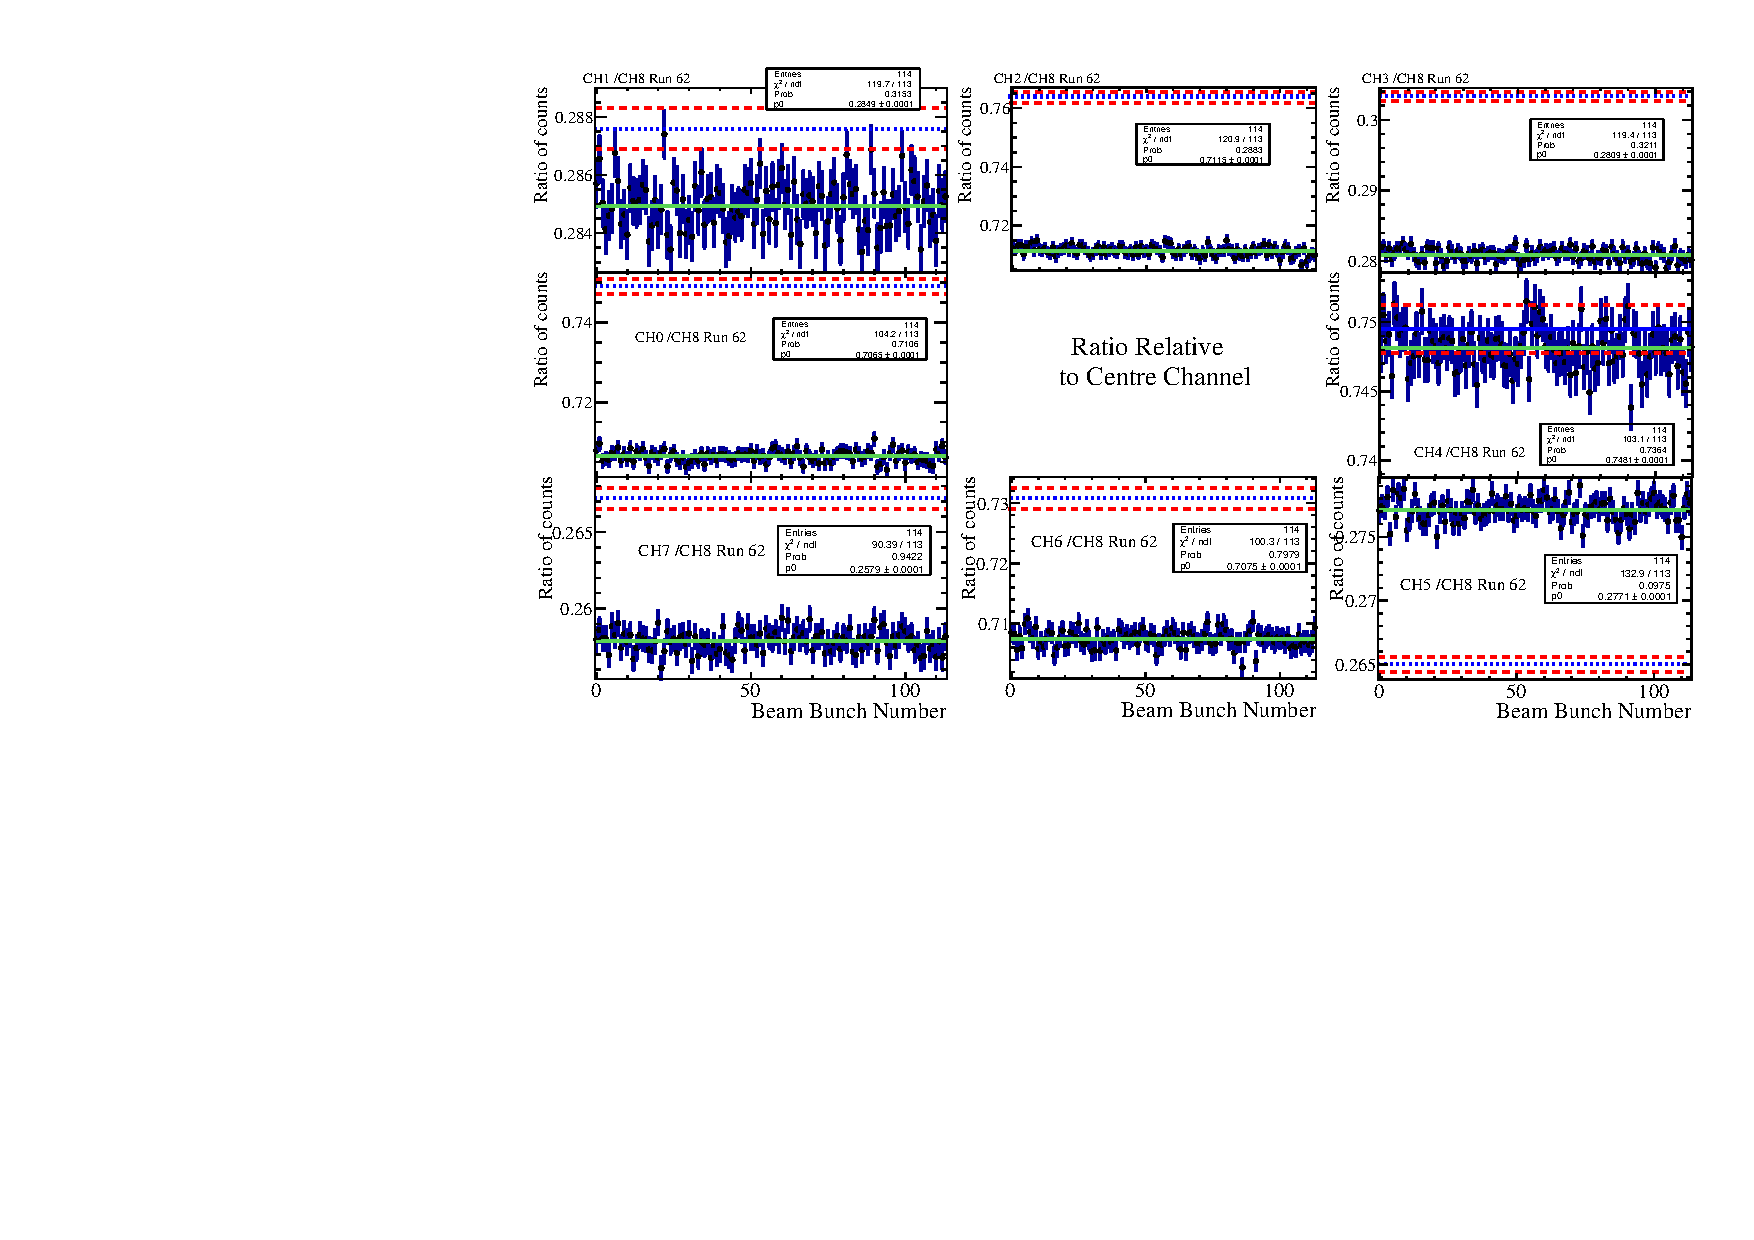
\includegraphics[width=0.95\textwidth]{figures/relratios.pdf}
\caption{ Count ratio of each channel relative to the central channel
  are shown (data points), and fit to a constant (green-solid lines).
  The relative area exposed to UCN is shown as a blue-dotted line with
  uncertainy given by the red-dashed lines.}
\label{fig:relratios}
\end{figure*}

\begin{table*}[ht]
  \caption{Relative to central channel (Ch.8) area compared to count of each of the detector channels}
  \centering
  \begin{tabular}{c | c c | c}
    \hline \hline
 Channel  & Norm. area ($A_N$)  & Norm. count ($N_C$)  &     $( A_N - N_C )$ \\    
    \hline 
    0  &      0.7490 $\pm$   0.0018   &    0.7065 $\pm$   0.0001    &        0.0425 $\pm$   0.0018\\
    1  &      0.2876 $\pm$   0.0007   &    0.2849 $\pm$   0.0001    &        0.0027 $\pm$   0.0007\\
    2  &      0.7634 $\pm$   0.0018   &    0.7115 $\pm$   0.0001    &        0.0519 $\pm$   0.0018\\
    3  &      0.3033 $\pm$   0.0006   &    0.2809 $\pm$   0.0001    &        0.0224 $\pm$   0.0006\\
    4  &      0.7495 $\pm$   0.0017   &    0.7481 $\pm$   0.0001    &        0.0014 $\pm$   0.0017\\
    5  &      0.2650 $\pm$   0.0006   &    0.2771 $\pm$   0.0001    &       -0.0121 $\pm$   0.0006\\
    6  &      0.7307 $\pm$   0.0018   &    0.7075 $\pm$   0.0001    &        0.0232 $\pm$   0.0018\\
    7  &      0.2672 $\pm$   0.0007   &    0.2579 $\pm$   0.0001    &        0.0093 $\pm$   0.0007\\
    \hline
  \end{tabular}
\label{tab:relrates}
\end{table*}





\subsection{ Comparison to Cascade detector }

Both the Cascade and $^6$Li detectors were connected individually to
each of these ports and collected data.  PSI also had a
Y-configuration available which evenly split the beam between the
detectors as shown in Figure \ref{fig:yConfig}.  This allowed a more
direct comparison of the UCN rates, and forms the basis of the
comparison in this paper.

\begin{figure}[!htpb] 
\centering 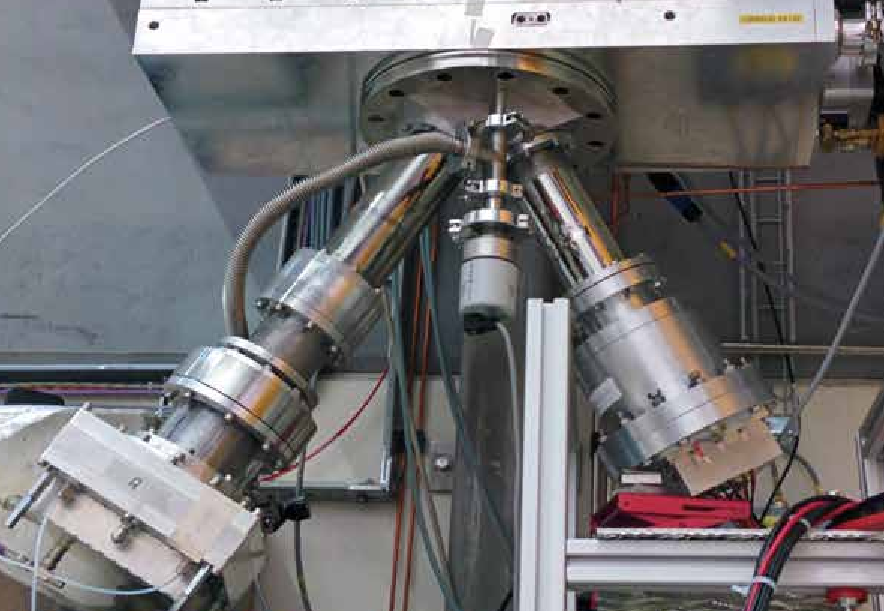
\includegraphics[width=0.49\textwidth]{figures/yConfig.pdf}
\caption{Configuration for splitting the UCN into two detectors.  The
  Cascade detector is on the left and the $^6$Li detector is on the
  right.}
\label{fig:yConfig}
\end{figure}


\subsection{Cascade Detector}

The Cascade UCN detector, typically used at PSI and other UCN
facilities is a GEM-based neutron detector with a single 200~nm thick
layer of $^{10}$B deposited on a 100~$\mu$m thick aluminum entrance
foil. The boron captures the neutron and releases an $\alpha$ and
$^7$Li particle,

\begin{equation}
^{10}B + n \rightarrow \alpha + {^7}Li.
\end{equation}

An Ar/CO$_2$ mixture is used as a detection gas.  Due to the low Z
materials, this detector picks up negligible $\gamma$ background. The
employed detector has a $10 \times 10$~cm$^2$ square shaped sensitive
area which is divided into 64 individually read out pixels.  The
detector comes with its own proprietary data acquisition system.  The
data acquisition is based on a complex pattern recognition algorithm
which is performed online in the detector's FPGA electronics.  This
allows the software to define, within a given range, what patterns are
accepted as a 'neutron' event.  A stacked type of Cascade counter is
more commonly used for cold and thermal neutron
counting\cite{cascade}.


%The Cascade data acquisition system runs on a windows computer and
%collects histograms binned in 0.1 second bins of the UCN count in each
%of the 64 pads (8x8) of the detector, along with a total count of UCN
%per 0.1 second time bin.  The electronics of the Cascade detector
%provides on board algorithms for counting multiple neutrons, and
%rejecting background events.


\subsection{Overview of the Measurement Method}

Both detectors were placed in the y-configuration at the West-2 port
to allow for a comparison of the averaged UCN rate over the course of
the beam cycle for both detectors for the same cycle.  The timing
calibration between the two detectors' Data AcQuisition (DAQ) was done
at the few second level by comparing the time reported by the DAQ
computers.  A more close matching of the time in the analysis of the
data was performed at about the 0.05~s level by aligning the times
when the UCN rate was increasing after the main proton beam
irradiation of the spallation target.

The gross timing is confirmed by looking at the total count of UCN
seen in each detector per proton beam irradiation cycle.  These counts
are correlated as are the times when a proton beam irradiation is
skipped and both detectors do not see UCN.
Figure~\ref{fig:ratecompare} shows the count of UCN detected in each
300 s cycle by each of the detectors.

Note that $^{6}$Li detector connects to the UCN source with a 75~mm
aperture to the UCN guide, while the Cascade detector connects with a
70~mm aperture.  To get a rough comparison of the two detectors, the
count seen by the $^{6}$Li detector is also shown scaled down by the
ratio of areas ($0.871$).  This comparison shows that the relative
count of UCN from the PSI source was changing over the course of this
data collection period, and that for the spectrum of UCN in this
beamline for the ${6}$Li detector is $10.279 \pm 0.024$(stat)\%.  The
y-configuration is as direct a comparison as could be obtained,
however simulations indicate there could be up to that large of a
difference in expected UCN rate due to uncertainties in the initial
UCN spectrum and the additional connectors required to reduce the
75~mm diameter guide to 70~mm diameter for the Cascade detector.
%Overall the lithium detector
%observed $8.28\pm0.02$(stat)$\pm$2.00(syst)\% more efficient for
%the UCN from the PSI source.

\begin{figure}[!htpb]
\centering 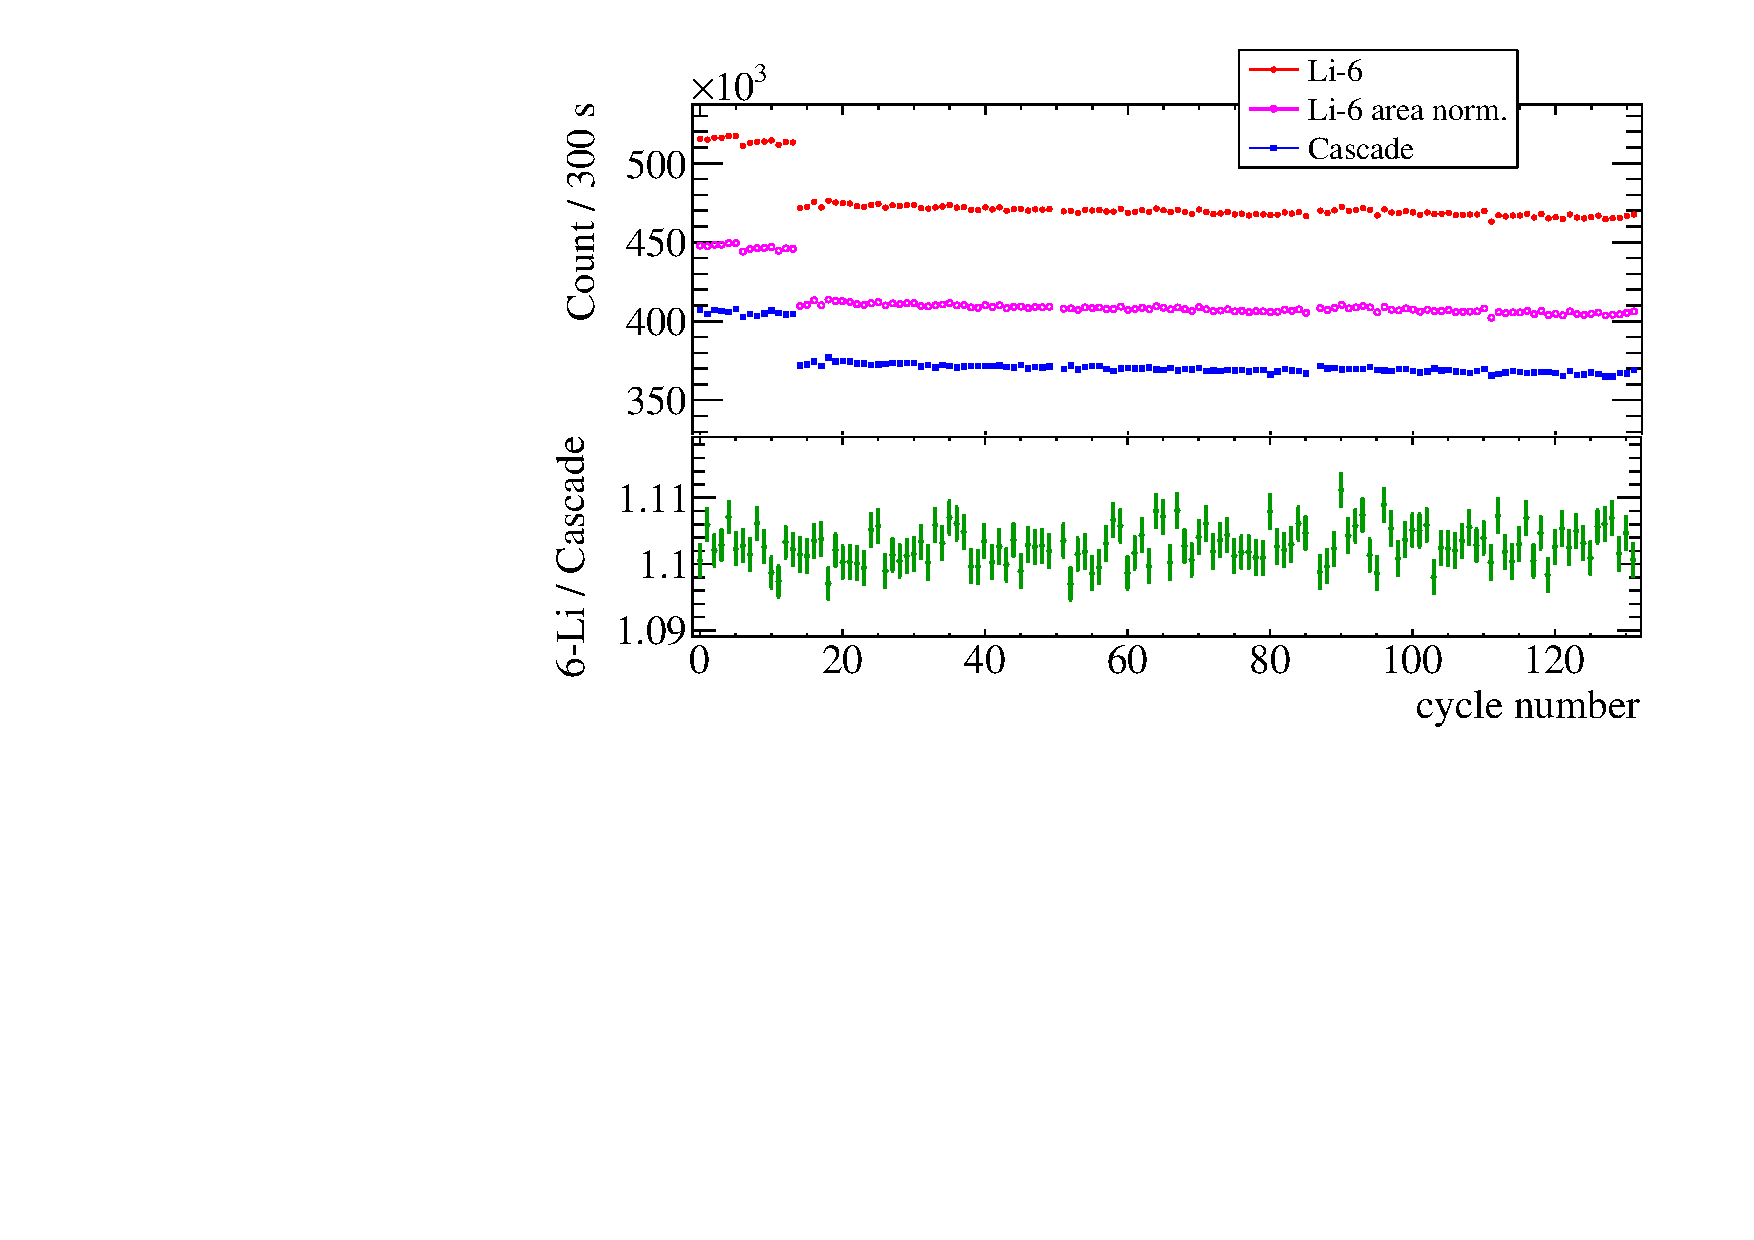
\includegraphics[width=0.49\textwidth]{figures/cascade_to_li_ratecompare.pdf}
\caption{Detected UCN count per 300 second cycle is shown in the top
  panel for the ${^6}$Li detector (red filled circles), Cascade
  detector (blue filled squares), and the area normalized ${^6}$Li
  count (magenta open circles).  The bottom panel shows the ratio of
  the area normalized count in the $^{6}$Li detector to the Cascade
  detector (colour online).}
\label{fig:ratecompare}
\end{figure}

In addition to the comparison of the count for a whole 300 second
cycle, the UCN detection rate in 0.1 second bins since the beginning
of the beam cycle averaged over 132 beam cycles is compared, as shown in
Fig.~\ref{fig:averagedRate}.  This comparison includes the area
normalization, and shows that the $^{6}$Li detector appears to detect
more UCN at higher rates at earlier times since the UCN production
than the Cascade detector.  We attribute the lower rate at later times
to the difference in the Fermi potential of the two detectors.  The
$^6$Li detector's lithium depleted glass, which is the first material
that the UCN see has a Fermi potential of 107~neV, while the Cascade
detector has an Al window with an effective Fermi potential of 54~neV.
The faster UCN reach the detectors sooner, and the $^6$Li detector's
performance for the higher energy UCN is better than the Cascade
detector.  However, later in the beam cycle, the UCN spectrum is
softer, and the lower energy UCN are not seen by $^{6}$Li detector,
making the Cascade detector more efficient for lower energy UCN (below
107~neV).

\begin{figure}[!htpb]
\centering 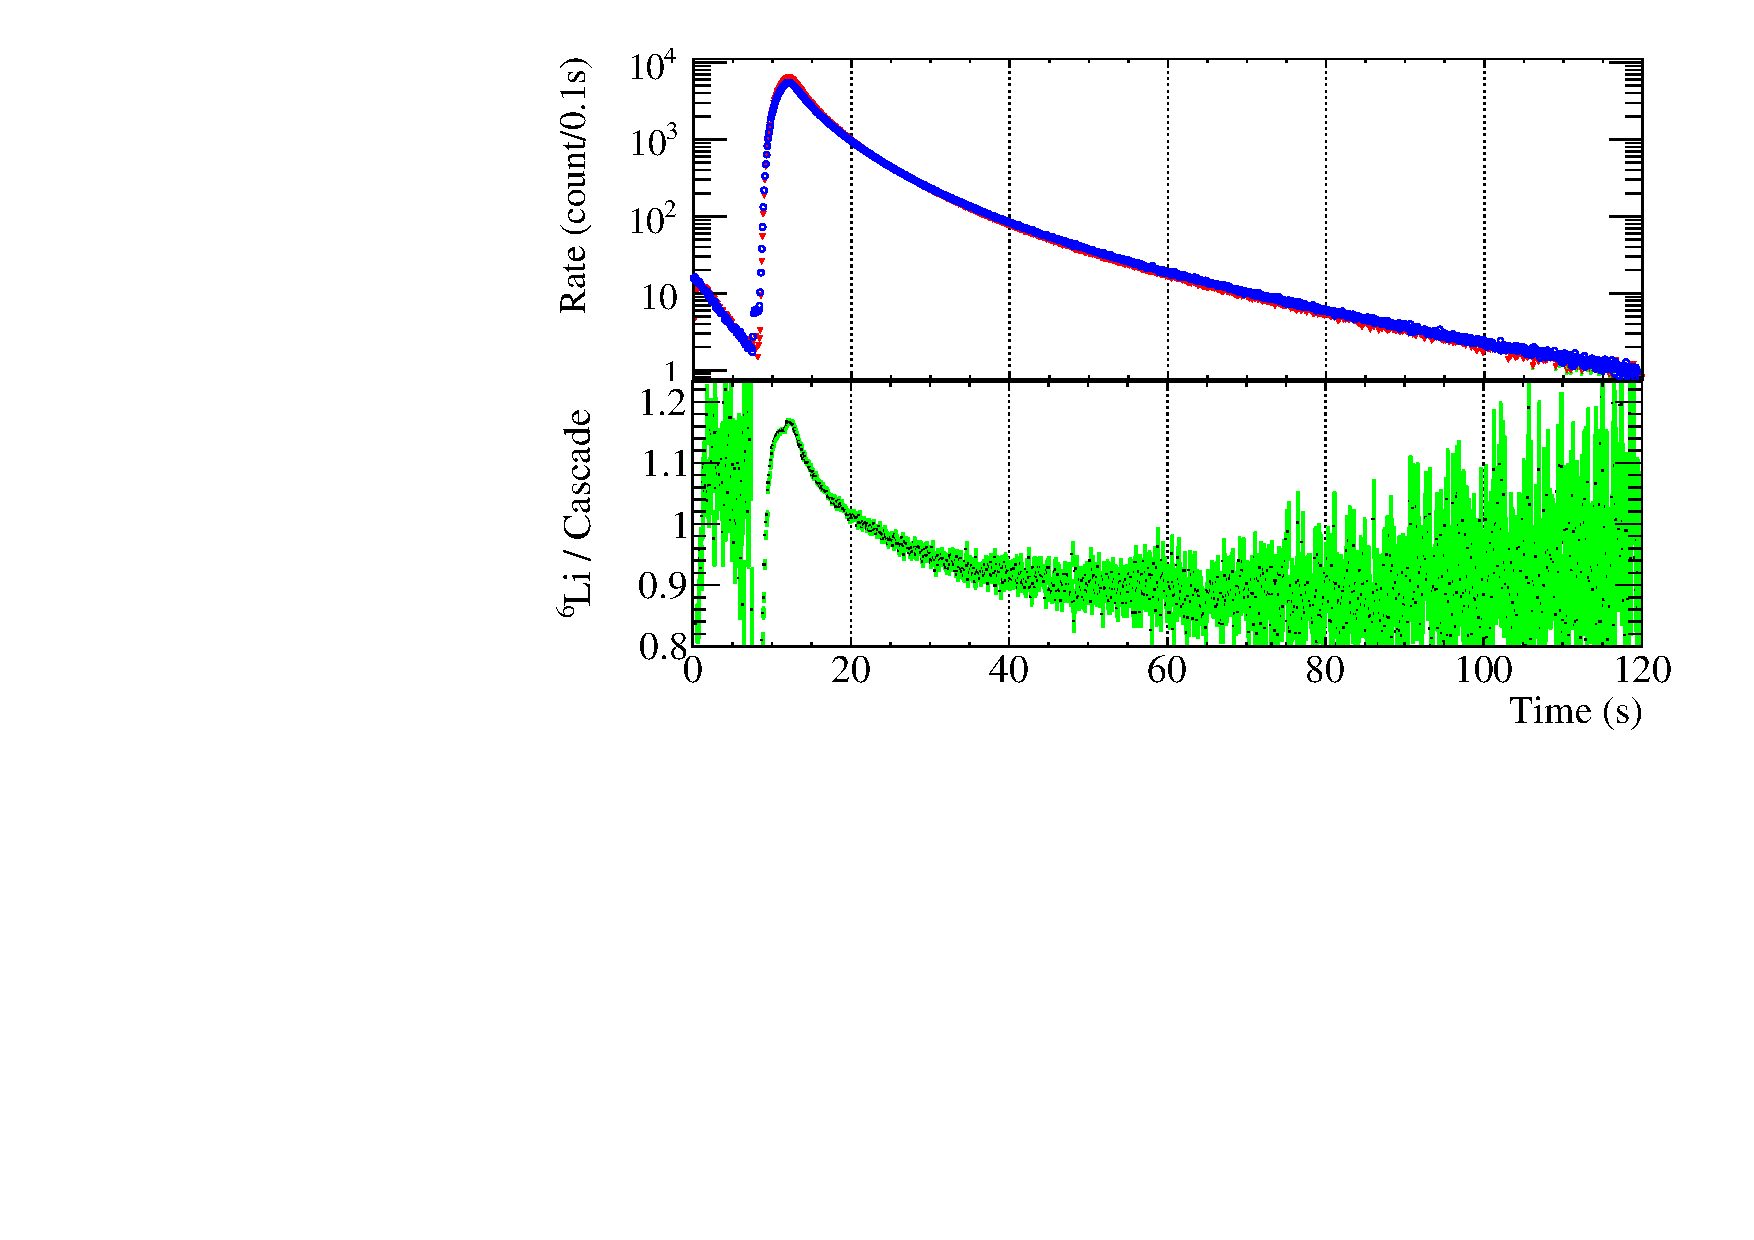
\includegraphics[width = 0.49\textwidth]{figures/cascade_to_li_130cycleavg.pdf}
\caption{UCN Detection count per 0.1s averaged over 130 UCN cycles.
  The top panel shows an overlay of the area normalized $^6$Li data in
  Red with the Cascade data in blue.  The bottom plot shows a ratio of
  $^6$Li count over Cascade count in each 0.1 s interval. }
\label{fig:averagedRate}
\end{figure}



% Concluding remarks
\section{Conclusion}

At high rates, the $^6$Li detector had a higher counting efficiency
than the Cascade detector.  At later times in the UCN production
cycle, which had a lower rate of UCN, the Cascade detector had a
higher counting efficiency.  This is explained as being due to the
higher efficiency of the $^{6}$Li detector for higher energy UCN
reaching the detector soon after the UCN production.  The lower
efficiency at late times is due to a softer UCN spectrum at late
times, and the higher Fermi potential of the lithium glass of
$107$~neV.  The $^6$Li detector has some sensitivity to background
radiation, which is reduced by PSD cuts to a level of $0.3\pm0.1$\%
for the rates of background seen at PSI.


\section*{References}

\bibliography{elsarticle-template}
%\bibliographystyle{elsarticle-num}
%\bibliographystyle{unsrt}

\appendix

\section{Calculating the number of pile-up and dead-time events}\label{sec:stats}

Consider two independent rates of events, a rate of signal events and
a rate of background events.  Given a running time and detection
window time, this section reviews the analytic calculation of the
number of single signal, single background, the various combinations
of multiple signal and background events, and the number of events
during the dead-time.

\subsection{Calculating the rates based on random Poisson processes}

Consider a rate of signal events, $R_{\tt sig}$.  For a given running
time, $T$, the number of expected signal events is $\nu_{\tt sig} =
R_{\tt sig} T$.  If a detector collects the signal over a gate with a
width in time, $t_{\tt LG}$, then in any of these gates the average
number of events in that time interval is $n_{\tt sig} = R_{\tt sig}$.
Each time the electronics triggers on a pulse from the detector it is
dead for a time $t_{\tt dead}$ after the width of the collection gate.

As a final effect, for some fraction of the events detected, there is
a second trigger (a re-trigger) on late light.  The number of these
events is some fixed fraction, $f_{\tt retrig}$, of the single signal
events.  This fraction depends on the signal event threshold, but once
determined for a given threshold, does not depend on the rate of
events (only on the total number of events).  The number of late light
re-triggers is:
\begin{equation}\label{eq:retrig}
\nu_{\tt retrig} = f_{\tt retrig} \nu_{1\tt sig}.
\end{equation}

The different combinations of events in a given running time, $T$,
that are being considered are those that have:
\begin{enumerate}
\item a single signal event, $\nu_{1\tt sig}$,     
\item multiple signal events, $\nu_{N\tt sig}$,    
\item a single background events, $\nu_{1\tt bg}$,
\item multiple background events, $\nu_{N\tt bg}$,
\item a single signal plus a single background event, $\nu_{\tt 1 sig 1 bg}$, and
\item one or more signal events during the dead-time, $\nu_{\tt dead}$. 
\end{enumerate}
The rate of signal and background events each has an expected average
number of events in any time interval that is a random process.

In any time interval, $T$, the number of single signal events
measured, $N_{1\tt sig}$, follows a Poisson distribution of the form:

\begin{equation*}
P( N_{1\tt sig} , \nu_{1\tt sig} ) = \exp{ \left( -\nu_{1\tt sig} \right) } \frac{ \nu_{1\tt sig}^{ N_{1\tt sig} } }{  N_{1\tt sig}! }.
\end{equation*}

The expected number of single signal events is defined to be:
\begin{equation} \label{eq:1sig}
\nu_{\tt 1 sig} = R_{\tt sig} T.
\end{equation}

Similarly, the number of single background events, $N_{1\tt bg}$,
follows a Poisson distribution:

\begin{equation*}
P( N_{1\tt bg}  , \nu_{1\tt bg} ) = \exp{ \left( -\nu_{1\tt bg} \right) } \frac{ \nu_{1\tt bg}^{ N_{1\tt bg} } }{  N_{1\tt bg}! }.
\end{equation*}

The expected number of single background events is defined to be:
\begin{equation} \label{eq:1bg}
\nu_{\tt 1 bg} = R_{\tt bg} T.
\end{equation}

For the multiple signal events in a single gate, consider the
probability of having more than one signal event in the time interval
of the gate.  In any randomly placed gate, the expected average number
of signal events is $\bar{ n }_{\tt sig} = t_{\tt LG} R_{\tt sig}$.
The gates are not randomly distributed, instead they occur if there
already was a signal event that triggered the gate.  Therefore for
each of the $N_{1\tt sig}$ signal events there is a probability of
having more than one additional signal event of:

\begin{equation*}
P( n_{\tt sig} > 0 , \bar{n}_{\tt sig} ) = 1 - P( 0, \bar{n}_{\tt sig} ) = 1 - \exp{ \left( -\bar{n}_{\tt sig} \right) } . 
\end{equation*}

This is one minus the probability of having zero extra signal pulses
in the gate.  The probability above is multiplied by the average
number of single signal events, giving the expected average number of
multiple signal triggers:

\begin{equation*}
\nu_{\tt N sig} = \nu_{\tt 1 sig} ( 1 - \exp{ \left( -\bar{n}_{\tt sig} \right) } ) .
\end{equation*}

Plug in the number of expected events in a randomly placed gate to get
the final result:

\begin{equation} \label{eq:Nsig} 
\nu_{\tt N sig} = \nu_{\tt 1 sig} ( 1 - \exp{ \left( -t_{\tt LG} \nu_{\tt 1 sig} / T \right) } ) .  
\end{equation}

Using a similar argument for multiple background events, on average,
the result is:
%\begin{equation}
\begin{align}\label{eq:Nbg}
\nu_{\tt N bg} &= \nu_{\tt 1 bg} ( 1 - \exp{ \left( -\bar{n}_{\tt bg} \right) } ) \nonumber \\
             &=  \nu_{\tt 1 bg} ( 1 - \exp{ \left( -t_{\tt LG} \nu_{\tt 1 bg} / T \right) } ).  
\end{align}
%\end{equation}

The number times we get a single neutron and a single gamma is
calculated as a sum of two terms.  The first term is the number of
times we get a single signal event times the probability of getting a
single background event in a randomly placed gate.  The second term is
the number of times we get a single background event times the
probability of getting a single signal event in a randomly placed
gate.  On average the number of these events is:

%\begin{equation}
\begin{align}
\nu_{\tt 1 sig 1 bg} &= 
           \nu_{\tt 1 sig} \exp{ \left( -t_{\tt LG} \nu_{\tt 1 bg} / T \right) } t_{\tt LG} \nu_{\tt 1 bg} / T + \nonumber \\
         & \nu_{\tt 1 bg} \exp{ \left( -t_{\tt LG} \nu_{\tt 1 sig} / T \right) } t_{\tt LG} \nu_{\tt 1 sig} /T.
\end{align}
%\end{equation}

Finally, the number of dead-time signal events, $\nu_{\tt dead}$, can
be calculated in a similar manner to the pile-up, $\nu_{\tt N sig}$.
Assume the total number of triggers is dominated by the single signal
or single background events: $\nu_{\tt 1 sig} + \nu_{\tt 1 bg}$.  For
each of these triggers, the average number of signal events during a
dead time is $\bar{n}_{\tt dead} = t_{\tt dead} R_{\tt sig}$.  Each of
the triggers has a Poisson probability of having one or more signal
events during the dead time:
%\begin{equation*}
\begin{align*}
P( n_{\tt dead} > 0, \bar{n}_{\tt dead} ) =& 1 -  P( 0, \bar{n}_{\tt dead} ) \nonumber \\
                                     =& 1 - \exp{ \left( -\bar{n}_{\tt dead} \right) } .
\end{align*}
%\end{equation*}

Again, this is just one minus the probability of having zero extra
signal pulses in the time period after any gate.  Multiply the above
probability times the number of triggers, and we expect, on average,
to have the number of dead-time neutrons:
\begin{equation}\label{eq:dead}
\nu_{\tt dead} = (\nu_{\tt 1 sig} + \nu_{\tt 1 bg} ) \cdot 
         ( 1 - \exp{ \left( -t_{\tt dead} \nu_{\tt 1 sig} / T \right) } ).
\end{equation}


\begin{figure}[!htpb]
\centering
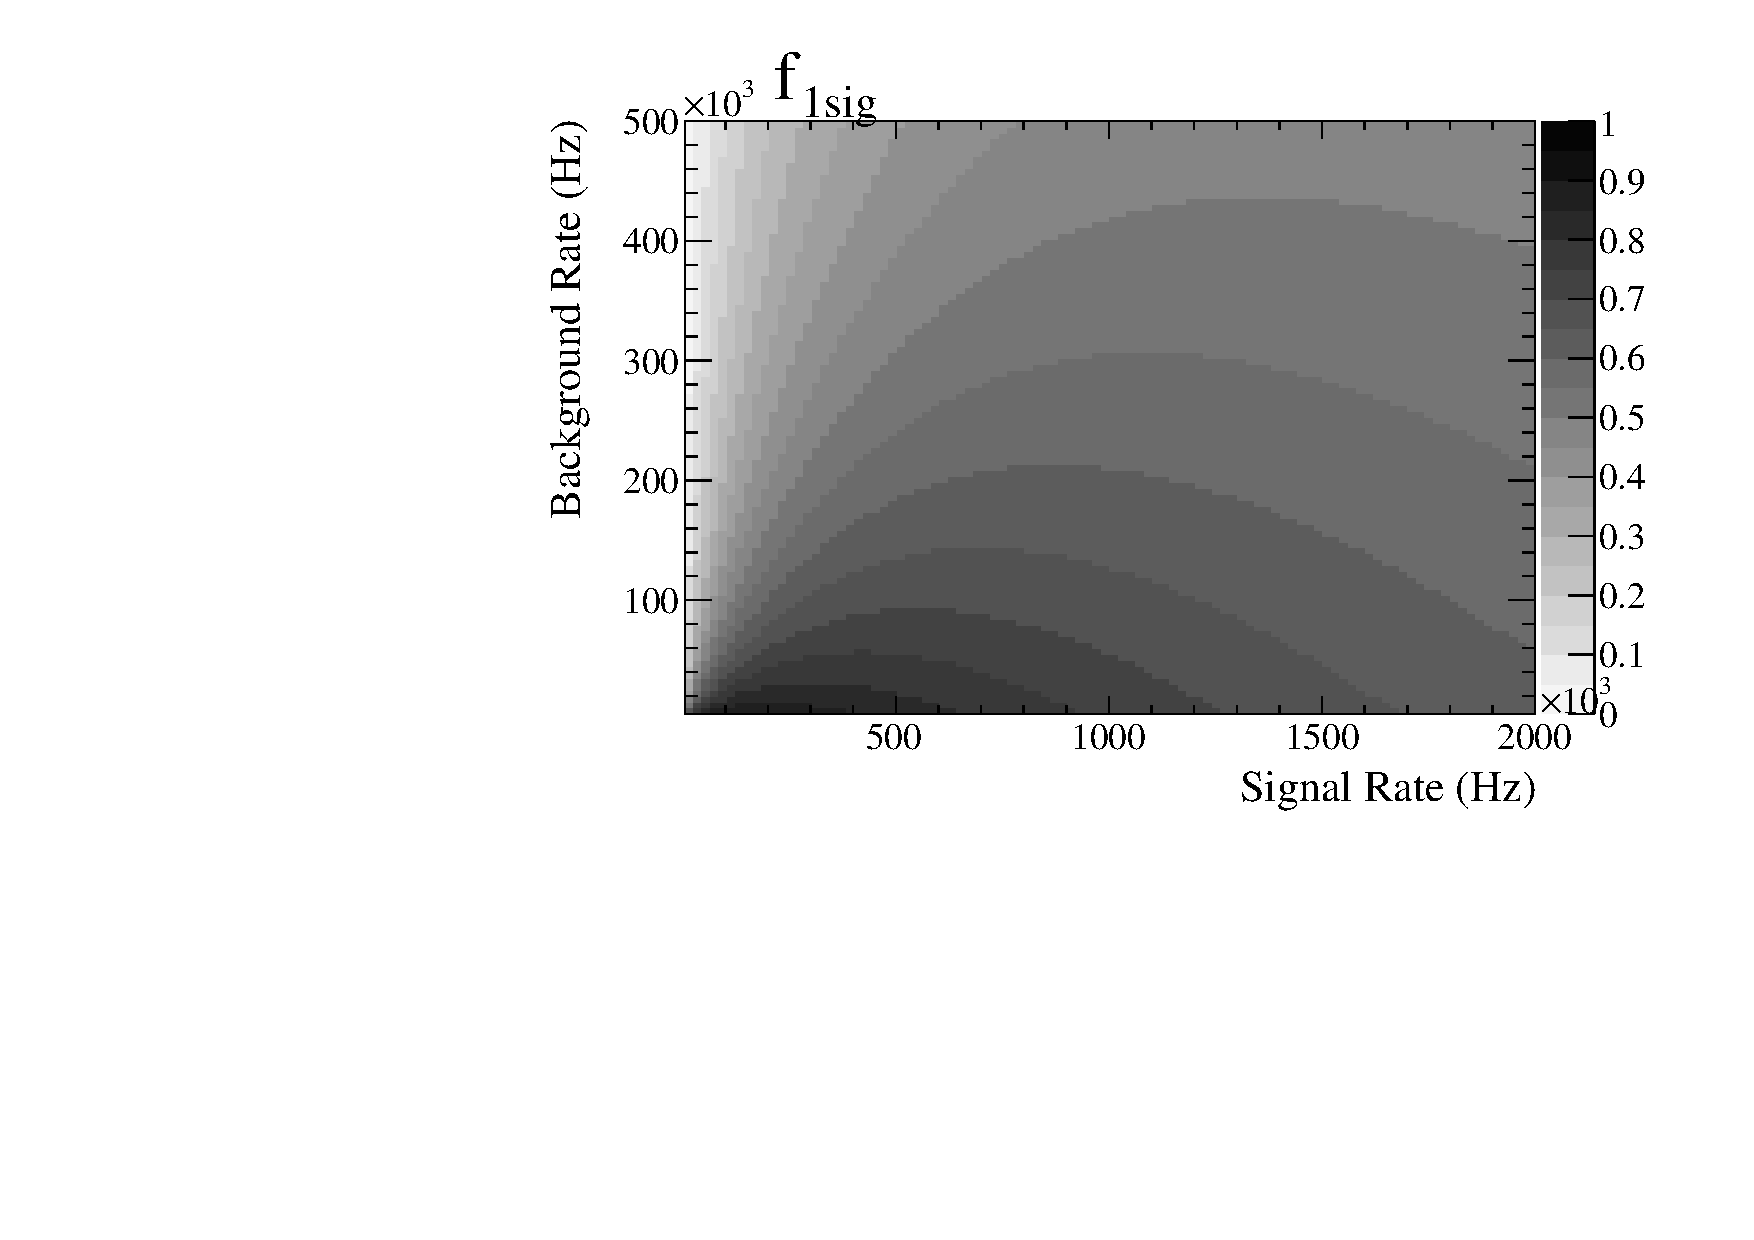
\includegraphics[width=.45\textwidth]{figures/tf1sig.pdf}
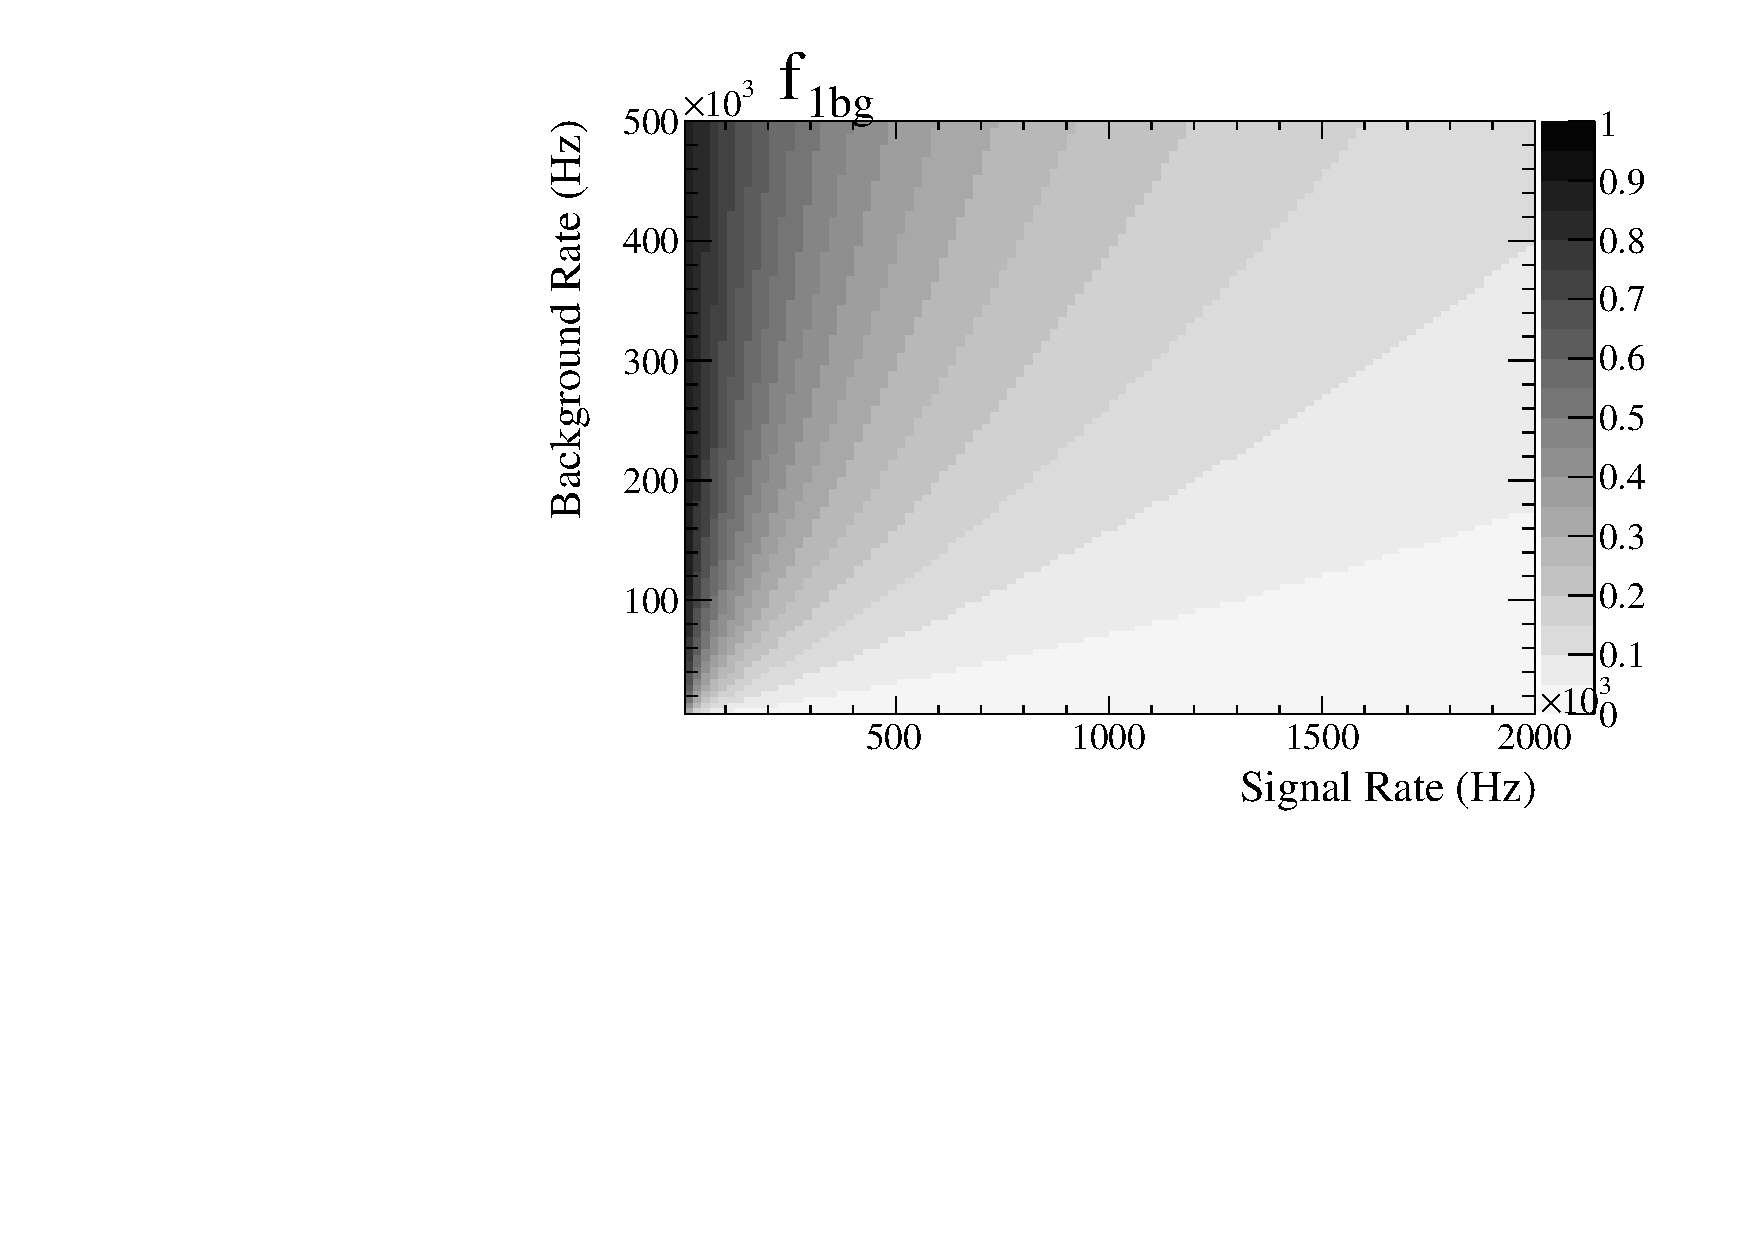
\includegraphics[width=.45\textwidth]{figures/tf1bg.pdf}
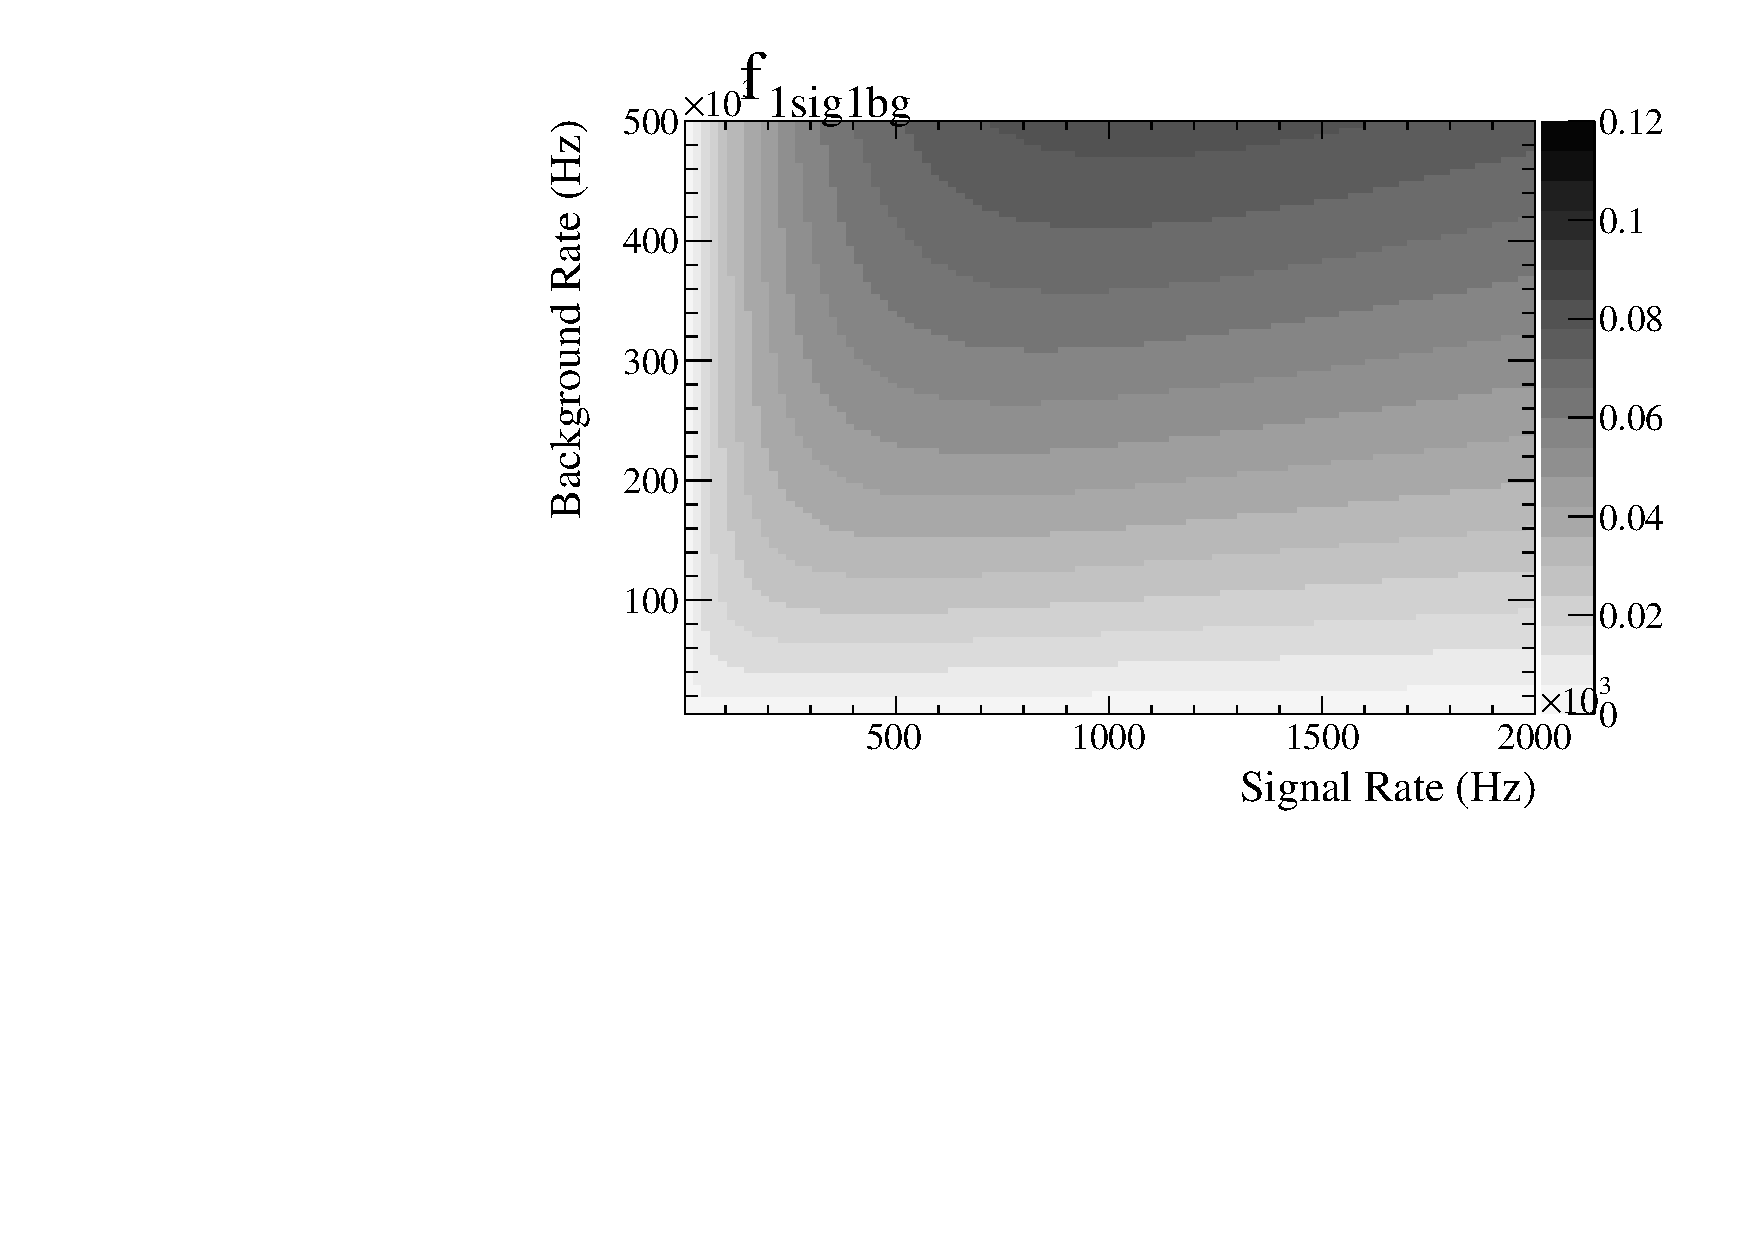
\includegraphics[width=.45\textwidth]{figures/tf1sig1bg.pdf}
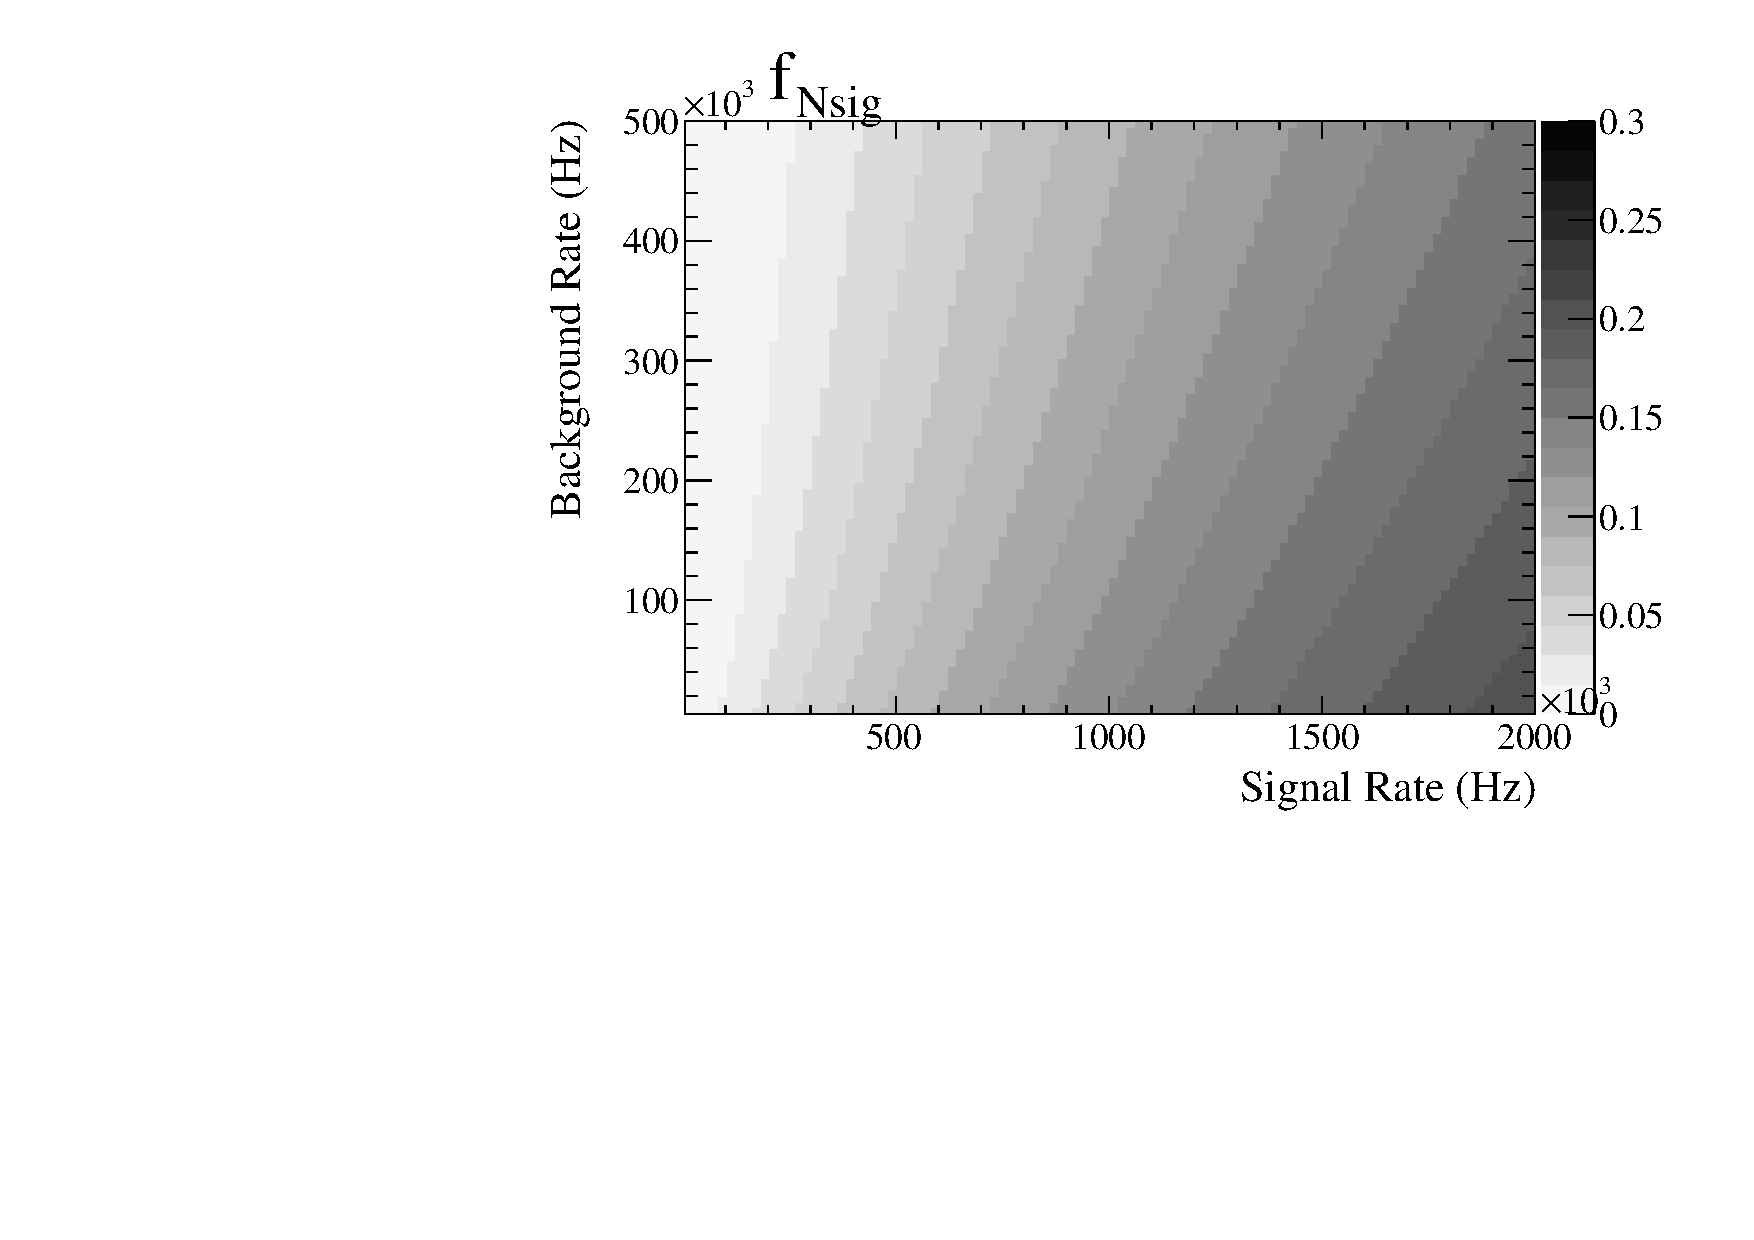
\includegraphics[width=.45\textwidth]{figures/tfNsig.pdf}
\caption{ Fraction of events as a function of rate, going from top to
  bottom are for: single signal events, single background events, 1
  signal and 1 background events, and multiple signal events.
}\label{fig:fracs}
\end{figure}



\begin{figure}[!htpb]
\centering
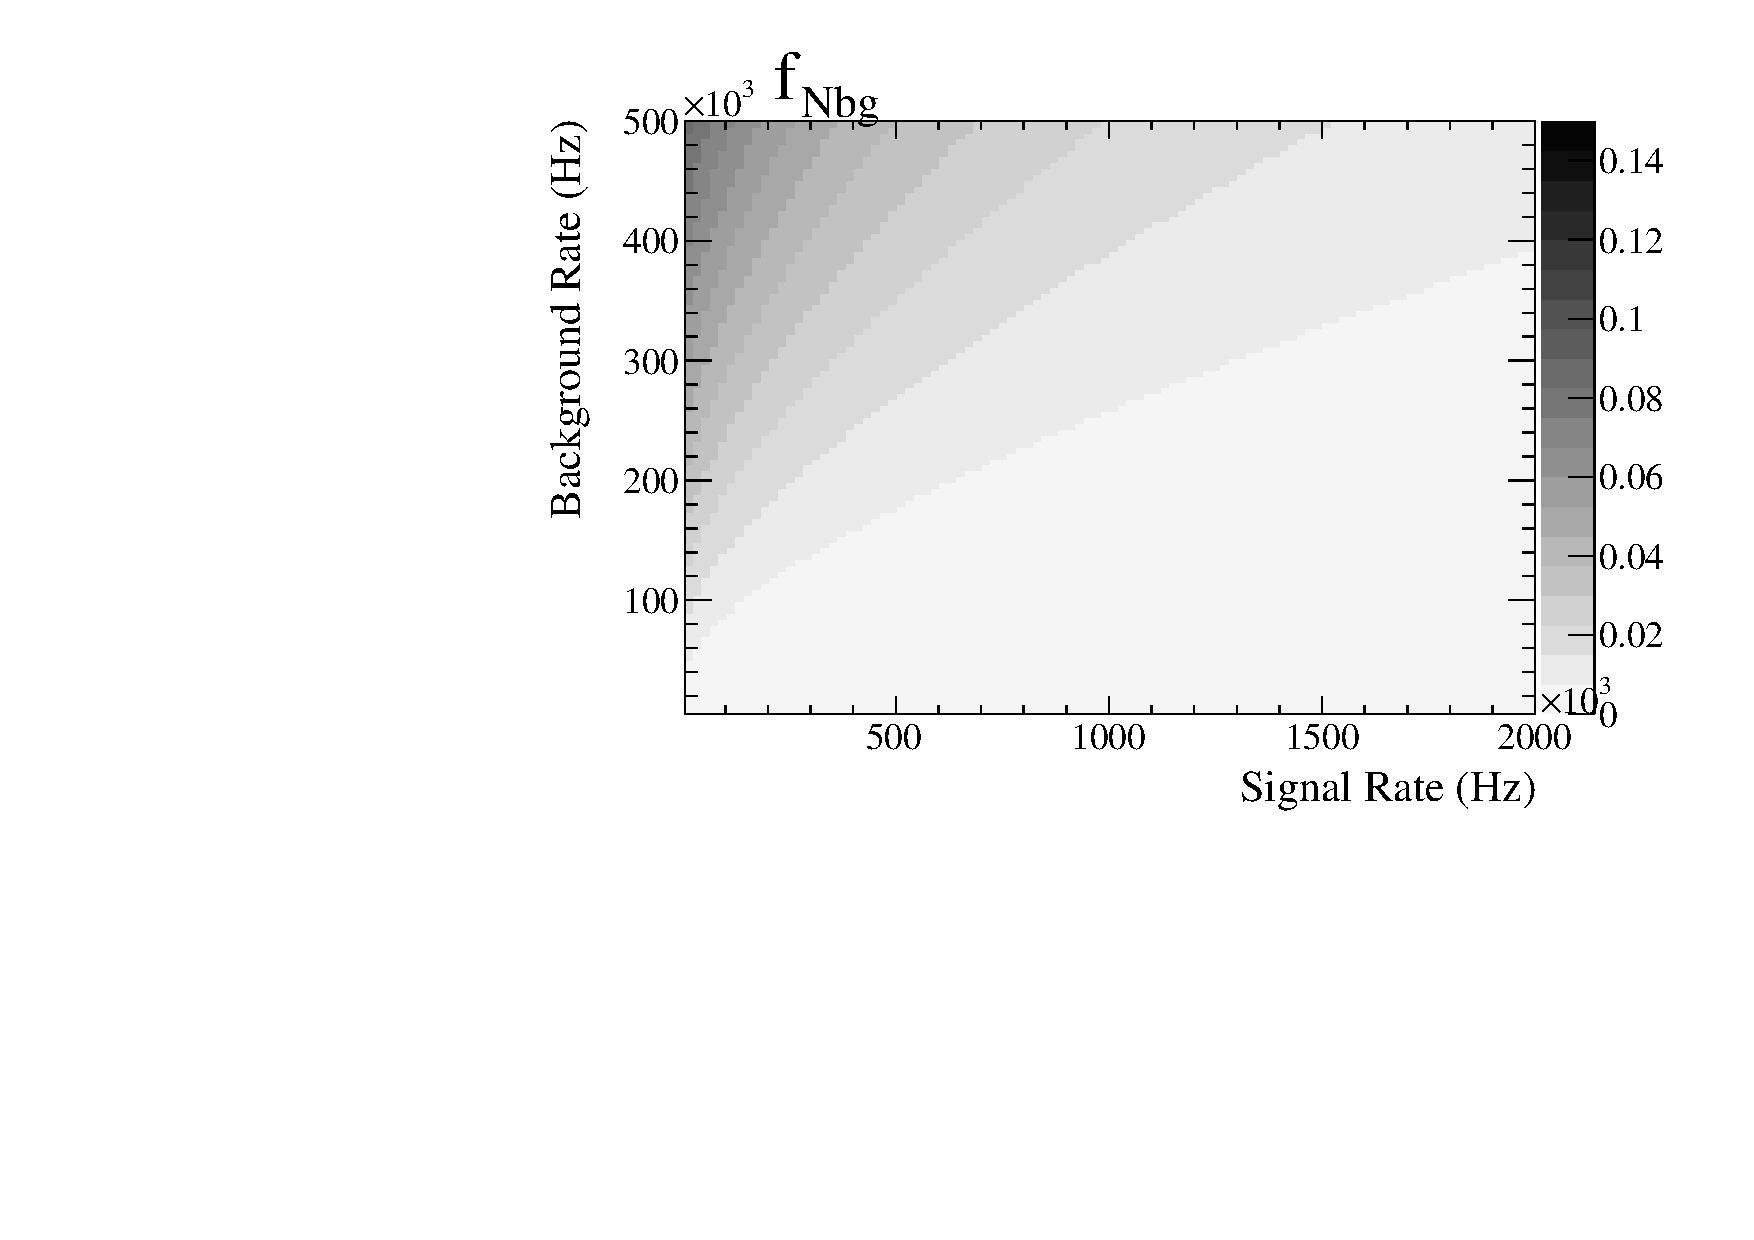
\includegraphics[width=0.49\textwidth]{figures/tfNbg.pdf}
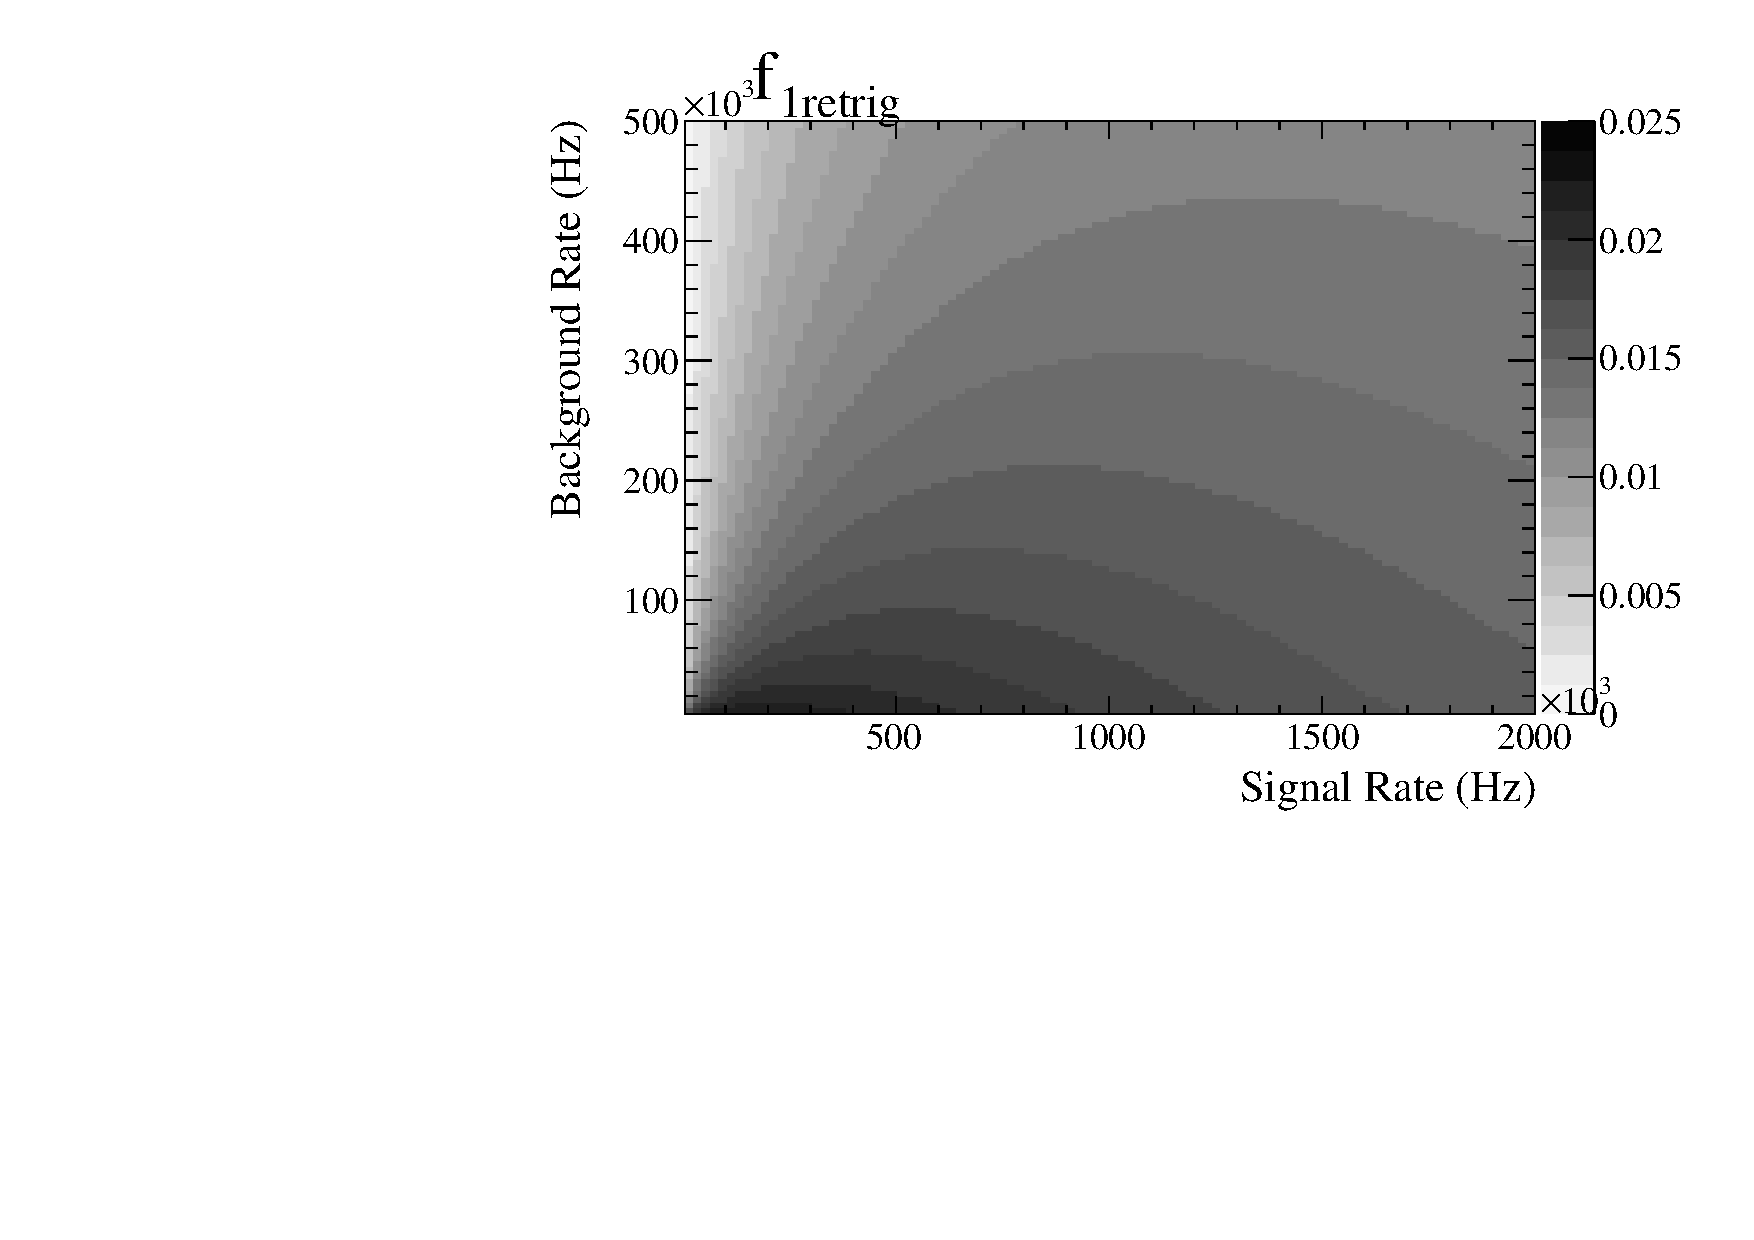
\includegraphics[width=0.49\textwidth]{figures/tf1retrig.pdf}
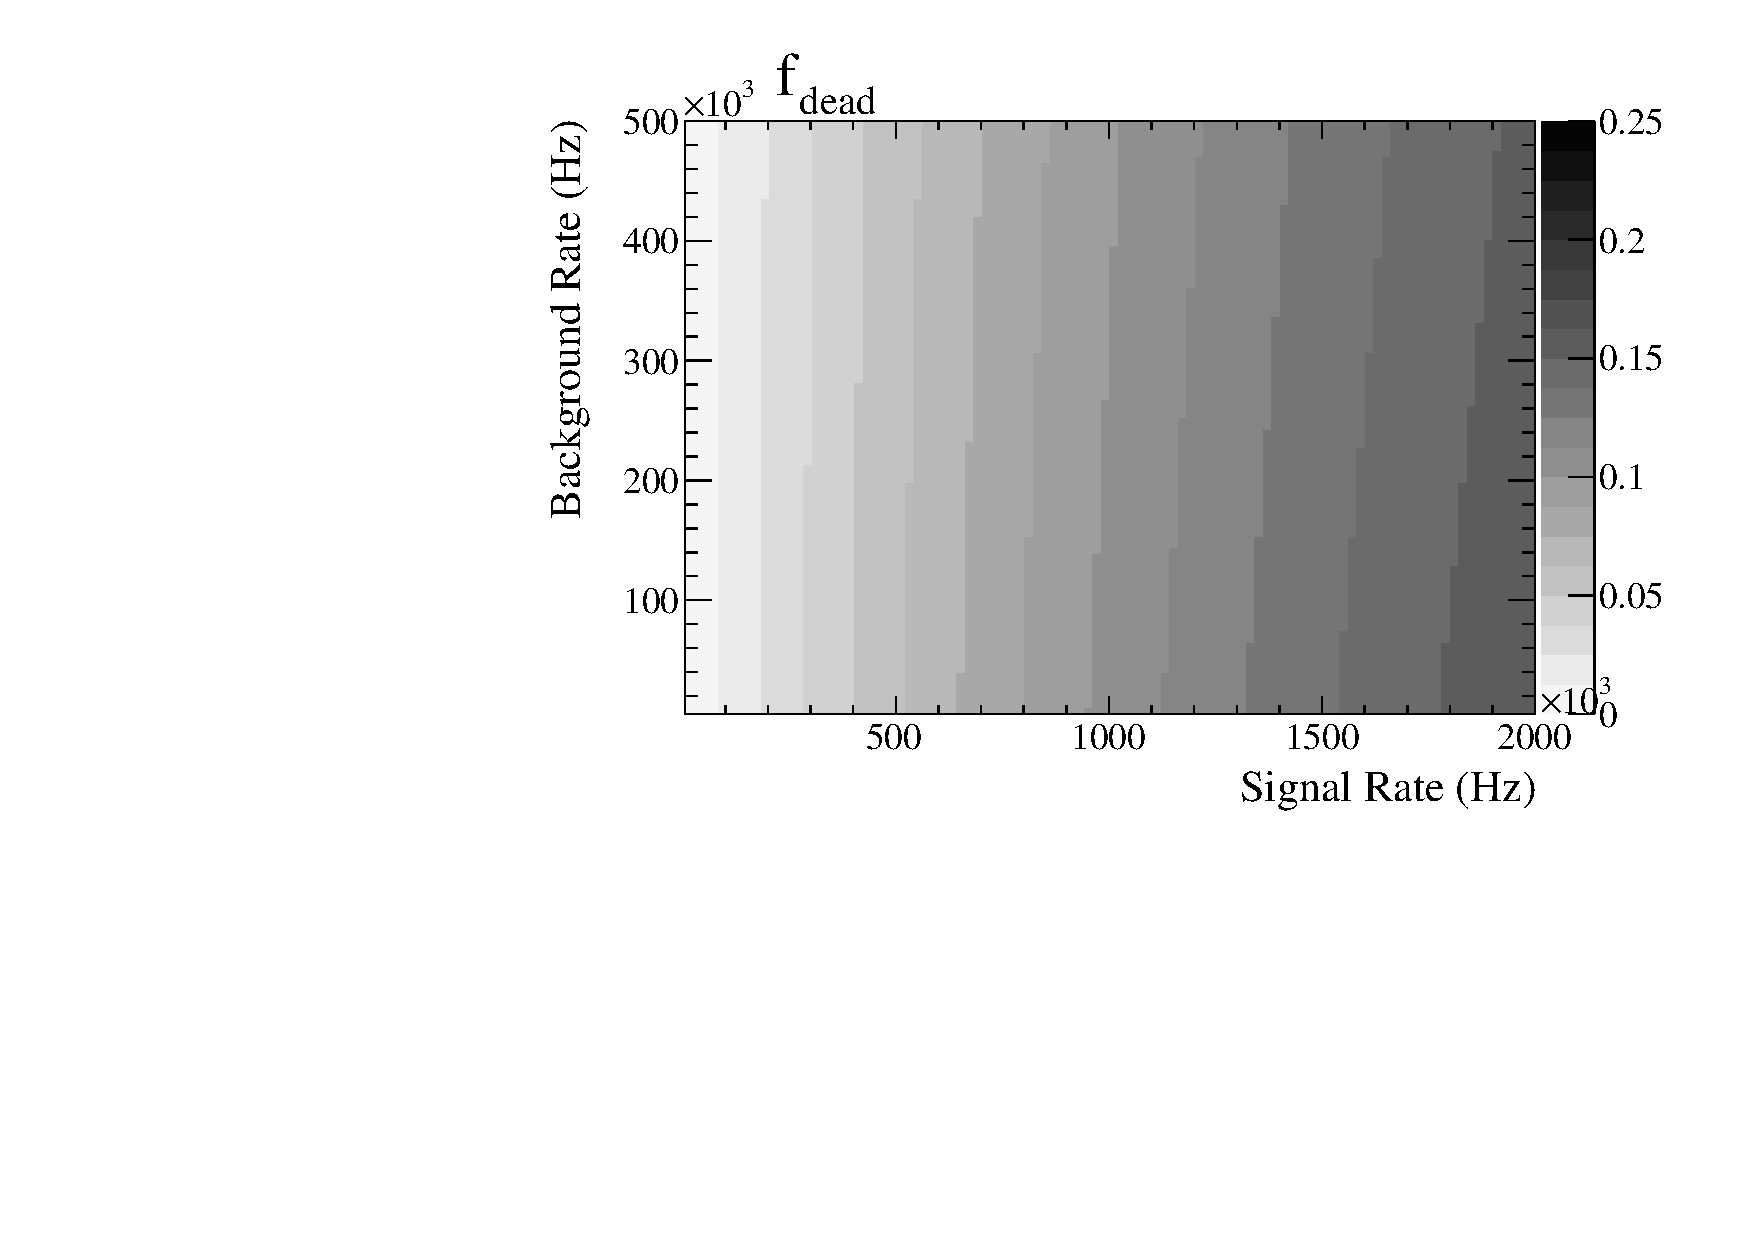
\includegraphics[width=0.49\textwidth]{figures/tfdead.pdf}

\caption{ Fraction of events as a function of rate, going from top to
  bottom are for: N background events, re-trigger on late light (set
  at 2.5\%), and dead time signal events.  }\label{fig:fracs2}
\end{figure}


\subsection{Calculations to test the rate equations}

In this section plots of the ratio of the number of events to the
total number of events as a function of signal rate and background
rate are plotted.  These plots are made as a contour map, with
$y$-axis being the signal rate, $R_{\tt sig}$, the $x$-axis being the
background rate, and the $z$-axis being the fraction of the triggers
of the given type.  These plots are made for each of the seven
categories of events.

For these plots we will use the settings that were used for the
digitizer in the measurements at PSI.  The relevant settings are,
$t_{\tt LG}=200$~ns, $t_{\tt dead}=150$~ns, and $f_{\tt retrig}=0.1$.
For these gate times, consider what happens when there is a high
signal rate of $R_{\tt sig} = 1/t_{\tt LG} = 5$~MHz with no
background.  After an arbitrary $T=10$~s of running at this rate the
number of single signal events is $\nu_{\tt 1 sig} = R_{\tt sig} T =
10^7$ events.  On average the number of times there is a multiple
signal events is given by Eq.~\ref{eq:Nsig}:
\begin{equation}
\nu_{\tt N sig} = 10^7 ( 1 - \exp{ \left( -2^{-7}\ {\tt s}\ \cdot 10^7  / 10\ {\tt s} \right) } ) = 1.8\times10^6. 
\end{equation}
This seems reasonable that there would be a large fraction of the
events ($\sim 18$\%) that would have more than one neutron.

In calculating the fractions of events we use for the denominator, the
total average (expected) number of triggers as a function of rate:

\begin{equation}\label{eq:N}
\nu = \nu_{1\tt sig} + \nu_{N\tt sig} + \nu_{1\tt bg} + \nu_{N\tt bg} + \nu_{\tt 1 sig 1 bg} + \nu_{\tt dead} + \nu_{\tt retrig}.
\end{equation}

In equation~\ref{eq:N} each term can be calculated using
Eqs. \ref{eq:retrig} to \ref{eq:dead}, which may depend on the signal
and background rates.  For example the fraction of single signal
events is then given by:

\begin{equation}
f_{\tt 1 sig } = \frac{ \nu_{\tt 1 sig} }{ \nu }.
\end{equation}

Similar expressions can be written for the fractions of each of the
event types.  Fig.~\ref{fig:fracs} and Fig.~\ref{fig:fracs2} show the
fraction of each type of event as a function of signal and background
rate.



\end{document}
